\chapter{MATRIZ DE COVARIÂNCIAS DOS ERROS DE PREVISÃO}
\label{cap:matriz_cov_estatica}

Na matriz de covariâncias dos erros de previsão estão representas as relações espaço-temporais (dentro de um período fixo no tempo) da variação dos erros de uma determinada variável e as relações que esta tem com outras variáveis a serem analisadas pelo sistema de assimilação de dados. As covariâncias dos erros de previsão representam, portanto, uma espécie de climatologia dos erros da previsão do modelo. Diferentes técnicas foram propostas para a determinação destas covariâncias, sendo a mais largamente utilizada aquela denominada de método \textit{National Modeling Center} (NMC), introduzida por \citeonline{parrishederber/1992}. Outras técnicas incluem o método observacional \cite{hollinsgsworthelonnberg/1986} e mais recentemente, o método por conjunto \cite{fisher/2003}. O método de \citeonline{hollinsgsworthelonnberg/1986} é baseado nas medidas do termo de inovação (i.e., $\mathbf{y}^{o}-\mathbf{H}(\mathbf{x}^{b})$) e é portanto dependente das observações, além do modelo. Se as observações consideradas forem exatamente as mesmas representadas pelo modelo, então o operador observação é apenas um interpolador (na Seção \ref{sec:ex_anl_wind} é dado um exemplo de como o operador $H$ é aplicado no cálculo da análise do vento horizontal). Do contrário, o operador observação deve incluir também as relações físicas que permitem que estas quantidades possam ser relacionadas, portanto, tornando este método mais complicado e susceptível a erros. Por outro lado, ao invés de se considerar a diferença entre observações e previsões de curto prazo (e.g., 6 horas), o método NMC utiliza a diferença entre duas previsões (48 e 24 horas). Neste caso, não há necessidade de se utilizar um operador observação, visto que as quantidades avaliadas são oriundas do mesmo modelo. Uma das vantagens deste método em relação ao método observacional está, portanto, no fato de não serem necessárias observações para o cálculo das covariâncias. Consequentemente, a determinação das covariâncias para toda a grade global pode ser prejudicada sobre as regiões onde não se tem muitas observações (e.g., todo o HS, em relação ao HN), o que não deve acontecer com o método NMC, uma vez que este utiliza previsões para esta estimativa. O método por conjunto é semelhante ao método NMC no sentido do uso das informações do modelo para a estimativa das covariâncias. Porém, ao invés de utilizar a diferença entre pares de previsões, utiliza um conjunto delas para, de forma semelhante a Eq. \ref{eq:enkf_pb}.

Cada um destes métodos assume diferentes suposições, mas todos lidam com o fato de que não se conhece o verdadeiro estado da atmosfera e que uma amostragem deste verdadeiro estado é impossível.

\section{Importância da Matriz B}
\label{sec:import_B}

Para se verificar a importância da matriz de covariâncias dos erros de previsão ($\mathbf{B}$), pode-se tomar por base a Eq. \ref{eq:fcusto}, supondo-se apenas uma observação e um ponto de grade a ser analisado e que o operador observação seja linear ($\mathbf{H}$):

\begin{equation}
\label{eq:20}
J(\mathbf{x}) = \frac{1}{2} (\mathbf{x} - \mathbf{x}^{b})^{T} \mathbf{B}^{-1} (\mathbf{x} - \mathbf{x}^{b}) + \frac{1}{2} [\mathbf{y}^{o} - \mathbf{H}(\mathbf{x})]^{T} \mathbf{R}^{-1} [\mathbf{y}^{o} - \mathbf{H}(\mathbf{x})] \end{equation}

Neste caso mais simples, consideramos o operador observação como sendo,

\begin{equation}
\label{eq:21}
\mathbf{H}=[0,\dots,0,1,0,\dots,0]
\end{equation}

Partindo-se da Eq. \ref{apI_eq:22} com o operador observação linear, obtém-se:

\begin{equation}
\label{eq:22}
0 = (\mathbf{B}^{-1} + \mathbf{H}^{T}\mathbf{R}^{-1}\mathbf{H})(\mathbf{x}^{a} - \mathbf{x}^{b}) - (\mathbf{H}^{T}\mathbf{R}^{-1})[\mathbf{y}^{o} - \mathbf{H}(\mathbf{x}^{b})]
\end{equation}

Resolvendo-se a Eq. \ref{eq:22} para o incremento de análise ($\mathbf{x}^{a} - \mathbf{x}^{b}$), obtemos:

\begin{align}
    \label{eq:22_1}
    (\mathbf{B}^{-1} + \mathbf{H}^{T}\mathbf{R}^{-1}\mathbf{H})(\mathbf{x}^{a} - \mathbf{x}^{b}) & = (\mathbf{H}^{T}\mathbf{R}^{-1})[\mathbf{y}^{o} - \mathbf{H}(\mathbf{x}^{b})] \\
    \label{eq:22_2}
    \mathbf{x}^{a} - \mathbf{x}^{b} & = \frac{\mathbf{H}^{T}\mathbf{R}^{-1}[\mathbf{y}^{o} - \mathbf{H}(\mathbf{x}^{b})]}{\mathbf{B}^{-1} + \mathbf{H}^{T}\mathbf{R}^{-1}\mathbf{H}}
\end{align}

Multiplicando-se e dividindo-se por $\mathbf{B}$ o lado direito da Eq. \ref{eq:22_2}, obtemos:

\begin{align}
    \label{eq:22_3}
    \mathbf{x}^{a} - \mathbf{x}^{b} & = \frac{\mathbf{B}\mathbf{H}^{T}\mathbf{R}^{-1}[\mathbf{y}^{o} - \mathbf{H}(\mathbf{x}^{b})]}{1 + \mathbf{B}\mathbf{H}^{T}\mathbf{R}^{-1}\mathbf{H}} \\
    \label{eq:22_4}
    \mathbf{x}^{a} - \mathbf{x}^{b} & = \frac{\mathbf{B}\mathbf{H}^{T}\mathbf{R}^{-1}[\mathbf{y}^{o} - \mathbf{H}(\mathbf{x}^{b})]}{\frac{\mathbf{R} + \mathbf{H}\mathbf{B}\mathbf{H}^{T}}{\mathbf{R}}} \\
    \label{eq:22_5}
    \mathbf{x}^{a} - \mathbf{x}^{b} & = \frac{\mathbf{B}\mathbf{H}^{T}[\mathbf{y}^{o} - \mathbf{H}(\mathbf{x}^{b})]}{\mathbf{R} + \mathbf{H}\mathbf{B}\mathbf{H}^{T}}
\end{align}

Como a suposição inicial foi a de que há apenas uma observação e apenas um ponto de grade a ser analisado,  os termos $\mathbf{y}^{o} - \mathbf{H}(\mathbf{x}^{b})$ e $\mathbf{R} + \mathbf{H}\mathbf{B}\mathbf{H}^{T}$ são escalares. Com isso, pode-se afirmar que:

\begin{equation}
\label{eq:24}
\mathbf{x}^{a}-\mathbf{x}^{b} \propto \mathbf{BH}^{T}
\end{equation}

Ou seja, o incremento de análise $\mathbf{x}^{a}-\mathbf{x}^{b}$ é proporcional a uma coluna da matriz $\mathbf{B}$. O papel da matriz de covariâncias dos erros de previsão é o de localizar o incremento de análise espalhando a informação das observações e garantir que estes incrementos sejam dinamicamente consistentes nas dimensões horizontal e vertical.

\section{Método \textit{National Modeling Center} (NMC)}
\label{sec:met_NMC}

Para a aplicação do sistema híbrido 3DVar no contexto deste trabalho, foi determinada uma matriz de covariâncias para uso nos experimentos de acordo com a resolução escolhida. O método utilizado para a determinação da matriz de covariâncias, é o método conhecido como \textit{National Modeling Center} (NMC) \cite{parrishederber/1992}. Este método foi escolhido pelas seguintes razões:

\begin{enumerate}
    \item É um método relativamente simples de ser empregado, pois requer apenas a utilização das previsões de 24 e 48 horas do modelo;
    \item Pode ser empregado para calcular a matriz de covariâncias apenas para o período de estudo proposto (não requer uma base de dados de previsão excessivamente extensa);
    \item É o método geralmente escolhido para calcular a matriz de covariâncias do GSI no NCEP e em outros centros operacionais que utilizam este sistema.
\end{enumerate}

O método NMC supõe que a correlação espacial dos erros de previsão são semelhantes as correlações temporais entre as diferenças das previsões de 48 e 24 horas. Ou seja, a ideia principal do método NMC é escolher os erros que crescem mais rápido a partir das diferenças entre as previsões de 48 e 24 horas para uma grade global (ou entre as previsões de mais curto prazo para uma grade regional, considerando que a taxa de crescimento dos erros pode ser mais acentuada devido a erros na representação de processos de subgrade). A seguir será apresentado um algoritmo para o cálculo da matriz de covariâncias dos erros do previsão.

O cálculo da matriz de covariâncias dos erros de previsão para o modelo de circulação geral da atmosfera do CPTEC (MCGAv4 e BAMv0), segue um algorítimo semelhante ao proposto pela ferramenta ``gen\_be'' \cite{rizvietal/2009} desenvolvida pelo \textit{Developmental Testbed Center} (DTC) do \textit{National Center for Atmospheric Research} (NCAR), com a diferença de que este algoritmo não considera as variáveis de controle conteúdo de água líquida ($cw$), ozônio ($oz$) e temperatura da superfície do mar ($sst$), que são necessárias para o cálculo para um modelo espectral global. O algoritmo do programa ``gen\_be'' foi criado para calcular as estatísticas dos erros de previsão do modelo Weather Research and Forecasting Model (WRF), sendo empregado na assimilação de dados com o sistema variacional do \textit{Weather Research and Forecasting model Data Assimilation} (WRFDA). Apesar disso, o algoritmo principal para o cálculo da matriz de covariâncias para os casos regional e global, é fundamentalmente o mesmo. Portanto, o algoritmo aqui apresentado a partir do programa ``gen\_be'' servirá como exemplo para o cálculo da matriz $\mathbf{B}$ da componente variacional do GSI.

O cálculo da matriz de covariâncias dos erros de previsão utilizando-se o método NMC, envolve as seguintes variáveis: velocidade potencial ($\chi$), função de corrente ($\psi$), temperatura do ar ($T$), umidade relativa ($q$) e pressão a superfície ($ps$). O algorítimo original utiliza as componentes $u$ e $v$ do vento para calcular as quantidades divergência ($D$) e vorticidade ($\zeta$) a partir das Eqs. \ref{eq:25} e \ref{eq:26} a seguir:

\begin{equation}
\label{eq:25}
D=\frac{\partial u}{\partial x} + \frac{\partial v}{\partial y}
\end{equation}

\begin{equation}
\label{eq:26}
\zeta=\frac{\partial v}{\partial x} - \frac{\partial u}{\partial y}
\end{equation}

Seguindo-se a equação de Poisson (Eqs. \ref{eq:27} e \ref{eq:28}), são calculadas as quantidades função de corrente ($\psi$) e velocidade potencial ($\chi$):

\begin{equation}
\label{eq:27}
\nabla^{2}{\psi}=\zeta
\end{equation}

\begin{equation}
\label{eq:28}
\nabla^{2}{\chi}=D
\end{equation}

Para o caso do modelo WRF, estes passos iniciais são necessários, uma vez que o modelo não escreve estas variáveis nos seus arquivos de previsão (e que são utilizados pelo software ``gen\_be''). Para o caso do modelo de circulação geral do CPTEC, este primeiro passo não é necessário uma vez que as quantidades velocidade potencial ($\chi$) e função de corrente ($\psi$) são prognosticadas pelo modelo. 

A seguir, o programa ``gen\_be'' calcula os coeficientes de regressão para a velocidade potencial, temperatura e pressão em superfície com relação a função de corrente. Estes coeficientes são calculados para posteriormente montar o campo de velocidade potencial desbalanceado (parte rápida do fluxo - e.g., ondas de gravidade), temperatura desbalanceada e pressão em superfície desbalanceada. Estes campos são obtidos subtraindo-se a parte balanceada (parte lenta do fluxo - eg., onda de Rossby) do campo completo ou total de cada variável. Depois, as variâncias e os comprimentos de escala (horizontal e vertical) são calculados para cada uma das variáveis de análise. Os comprimentos de escala horizontal e vertical são bastante importantes por representarem o papel da localização das covariâncias dos erros de previsão a serem utilizadas no cálculo dos incrementos de análise.

Como resultado, depois que o arquivo com os desvios padrões, amplitudes e comprimentos de escalas é escrito, obtém-se uma matriz do tipo bloco-diagonal - representada de forma idealizada pela Figura \ref{fig:1}) composta pelas variâncias de cada variável de estado na diagonal principal (no GSI estas variáveis são velocidade potencial ($\chi$), função de corrente ($\psi$), temperatura ($T$), umidade ($q$), ozônio ($oz$), conteúdo de água de nuvens ($cw$), pressão em superfície ($ps$) e temperatura da superfície do mar ($sst$). As submatrizes que compõem a matriz $\mathbf{B}$ representam autocovariâncias e covariâncias entre as variáveis.

\begin{figure}[H]
\caption{Morfologia idealizada da matriz de covariâncias dos erros de previsão ($\mathbf{B}$).}
\vspace{2mm}
\begin{center}
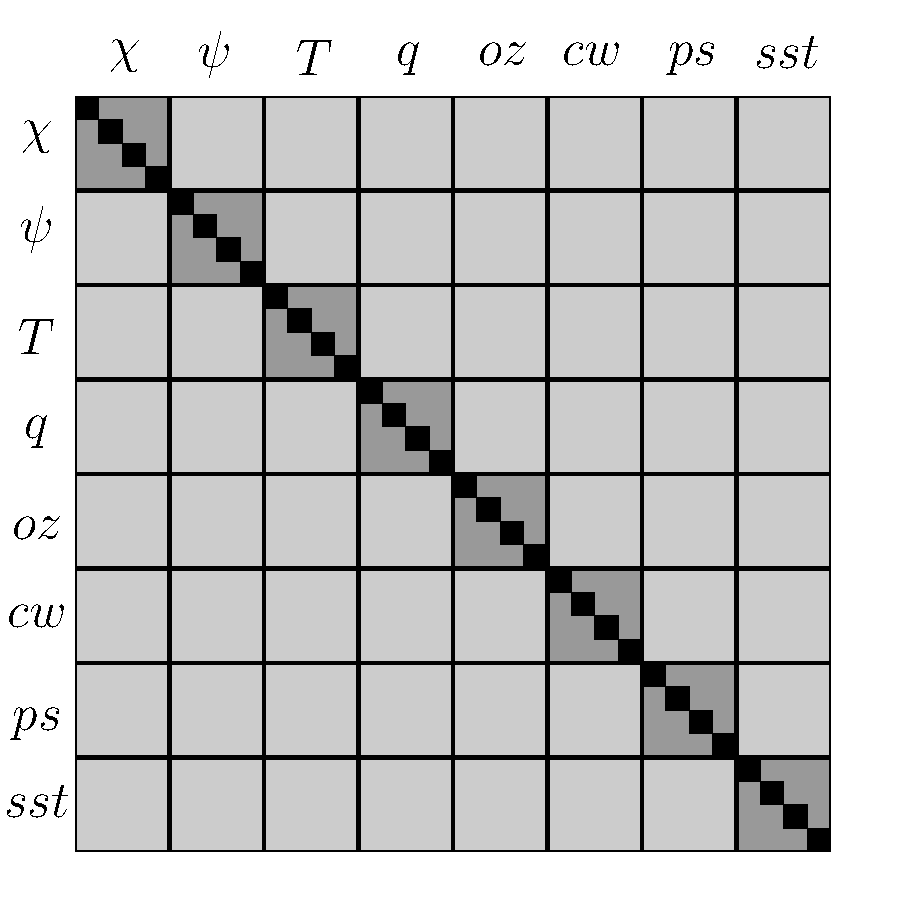
\includegraphics[scale=0.5]{./figs/cap3/matriz_B-new.pdf} 
\end{center}
 \vspace{2mm}
\legenda{No caso do GSI, as variáveis de estado analisadas são representadas: na diagonal principal os quadrados pretos representam as variâncias de cada variável; nos quadrados em cinza escuro, estão representados os elementos de autocovariância e em cinza claro, os elementos de covariância multivariados.}
\label{fig:1}
\FONTE{Adaptado de \citeonline{petrie/2012}}
\end{figure}

Para o cálculo da matriz de covariâncias do sistema GSI a partir do modelo de circulação geral do CPTEC, foram feitos dois testes. O primeiro teste considerou os pares de previsões de 48 e 24 horas que já estavam preparados na resolução TQ0299L064 (experimento denominado ``TAG'' - este experimento não faz parte do escopo deste trabalho) e extraídos do ciclo de assimilação de dados do sistema G3DVAR (versão 1.1.3) utilizando o modelo MCGAv4. O segundo teste considerou os pares de 48 e 24 horas do modelo BAMv0 na resolução TQ0062L028. Neste segundo teste, os pares de previsões foram obtidos a partir da realização do modelo BAMv0 usando as análises do NCEP. As justificativas para que o segundo teste tenha sido feito a com as análises do NCEP, são as seguintes: 1) foram encontradas inconsistências na representação das quantidades $oz$ e $cw$ na matriz de covariâncias quando esta foi calculada com base no MCGAv4; 2) embora seja possível calcular uma matriz de covariâncias para uma resolução menor do que a dos pares de entrada, estes pares não apresentaram valores consistentes de $oz$ e $cw$, fato este que não foi amenizado com a troca de resolução; 3) o problema com as quantidades $oz$ e $cw$ foi temporariamente resolvido utilizando-se as quantidades de $oz$ e $cw$ da matriz de covariâncias do NCEP, porém os primeiros testes do sistema híbrido 3DVar na resolução TQ0299L064 foram desencorajadores devido ao elevado custo computacional (e.g., dificuldades em alocar os recursos necessários para a realização dos membros do conjunto em tempo próximo do operacional); 4) não havia pares de previsões de 48 e 24 horas disponíveis para o MCGAv4 na resolução TQ0062L028 e portanto optou-se por testar uma versão mais recente do modelo de circulação geral do CPTEC (neste caso o modelo BAMv0) na tentativa de se sanar o problema com a representação de $oz$ e $cw$ (sem a necessidade de se copiar estas quantidades da matriz do NCEP) e facilitar a realização do sistema híbrido 3DVar. 

A matriz de covariâncias resultante do segundo teste foi então escolhida para a realização dos experimentos com o sistema híbrido 3DVar (cujos resultados são apresentados no Capítulo \ref{cap:resultados}). Nesta seção, portanto, são apresentadas as características principais das matrizes de covariâncias calculadas (nos dois testes mencionados), pois a matriz de covariâncias estática faz parte da metodologia aplicada ao longo deste trabalho.

O cálculo da matriz de covariâncias na resolução TQ0299L064 com os pares de previsões do modelo MCGAv4, foi feito com 1460 pares de previsões de 48 e 24 horas distribuídos ao longo de 1 ano (2013) no formato espectral. Os pares de previsões foram organizados na forma a seguir (válido também para a matriz de covariâncias do teste com o BAMv0): considerando-se o dia 2014010100, o primeiro par de previsões válido foi gerado com as análises dos dias 2013123100 (válido para uma previsão de 24 horas) e 2013123000 (válido para  uma previsão de 48 horas).

O algoritmo para o cálculo da matriz de covariâncias, cumpre as seguintes etapas:

\begin{enumerate}
    \item Leitura e organização dos pares de previsões de 48 e 24 horas;
	\item Remoção de viés (em toda a coluna vertical);
	\item Cálculo das matrizes de balanço que permitirão as transformações entre função de corrente ($\psi$) e as componentes desbalanceadas de velocidade potencial ($\chi$), pressão em superfície ($p$) e temperatura ($T$);
	\item Cálculo das variâncias dos erros de cada uma das variáveis de controle ($\psi$, $\chi$, $q$, $oz$, $cw$, $p$);
	\item Cálculo dos comprimentos de correlação verticais (em unidades inversas em ponto de grade);
	\item Cálculo dos comprimentos de correlação horizontais (em km).      
\end{enumerate}

No caso da matriz de covariâncias do MCGAv0 (na resolução TQ0299L064), nas etapas d), e) e f), as quantidades $oz$ e $cw$ foram posteriormente substituídas pelas quantidades correspondentes contidas na matriz de covariâncias do NCEP.

\section{Características Principais e Diagnósticos}

Nesta seção são apresentadas as características principais da matriz de covariâncias calculada no teste com o MCGAv4 (mencionado na seção anterior). As estruturas da matriz de covariâncias são apresentadas em termos de suas amplitudes. Como foram utilizados todos os pares de previsões de 48 e 24 horas disponíveis para o ano de 2013 na resolução TQ0299L028, foram calculadas também versões da matriz de covariâncias exclusivas para cada um dos horários sinóticos padrão (i.e., 00, 06, 12 e 18Z). Logo, uma comparação é feita entre estas versões da matriz de covariâncias do CPTEC com as versões completas das matrizes de covariâncias do CPTEC e NCEP. O objetivo destas comparações é caracterizar de forma quantitativa e qualitativa as matrizes calculadas. 

\subsection*{Características Principais da Matriz de Covariâncias do MCGA v4.x}

A matriz de covariâncias do GSI possui as seguintes estruturas: amplitudes (representadas por variâncias e desvios-padrão), distâncias (representadas pelos comprimentos de escalas horizontal e vertical) e matrizes de projeção de balanço. A matriz de covariâncias utilizada pelo CPTEC (3DVar) varia apenas nas latitudes e na vertical. As variáveis de estado do GSI são a função de corrente, a velocidade potencial desbalanceada, a temperatura virtual desbalanceada, a pressão em superfície, a pseudo umidade relativa (ou umidade relativa normalizada), a razão de mistura de ozônio e a razão de mistura de condensação em nuvens. Para cada uma destas variáveis são definidas amplitudes e as distâncias. As variáveis velocidade potencial, temperatura e pressão em superfície, possuem matrizes de projeção que são responsáveis por projetar o incremento da função de corrente no perfil da parte balanceada do incremento de cada uma destas quantidades. Para a velocidade potencial, uma matriz de correlação é utilizada para contabilizar a correlação positiva entre divergência e vorticidade.

Para se verificar a qualidade das amplitudes calculadas a partir dos pares de previsões do modelo de circulação geral MCGAv4 na resolução TQ0299L064, foram calculadas as amplitudes para os horários sinóticos padrão (00, 06, 12 e 18Z) e para todos os horários juntos (``AllZ''), para o período de 1 ano. Para este período de tempo, foi utilizado um total de 1460 pares (contabilizando todos os horários sinóticos) e 365 pares de previsões para as matrizes exclusivas de cada horário sinótico. Para comparação, foi utilizada a matriz de covariâncias do NCEP, calculada utilizando-se os pares de previsão do modelo GFS. Segundo \citeonline{wuetal/2002}, esta matriz foi calculada utilizando-se 49 pares de previsões, distribuídos ao longo de 1 ano. Em todos os casos, as comparações são feitas na grade de dimensões 768x386x64 (lon x lat x lev).

\begin{figure}[H]
    \caption{Distribuição das amplitudes calculadas para a matriz $\mathbf{B}$ na resolução TQ0299L064.}
    \vspace{2mm}
    \begin{center}
        \subfigure[$\mathbf{B}$ NCEP (ALLZ), $\psi$]{
          \label{fig:bncep_allz_psi}
          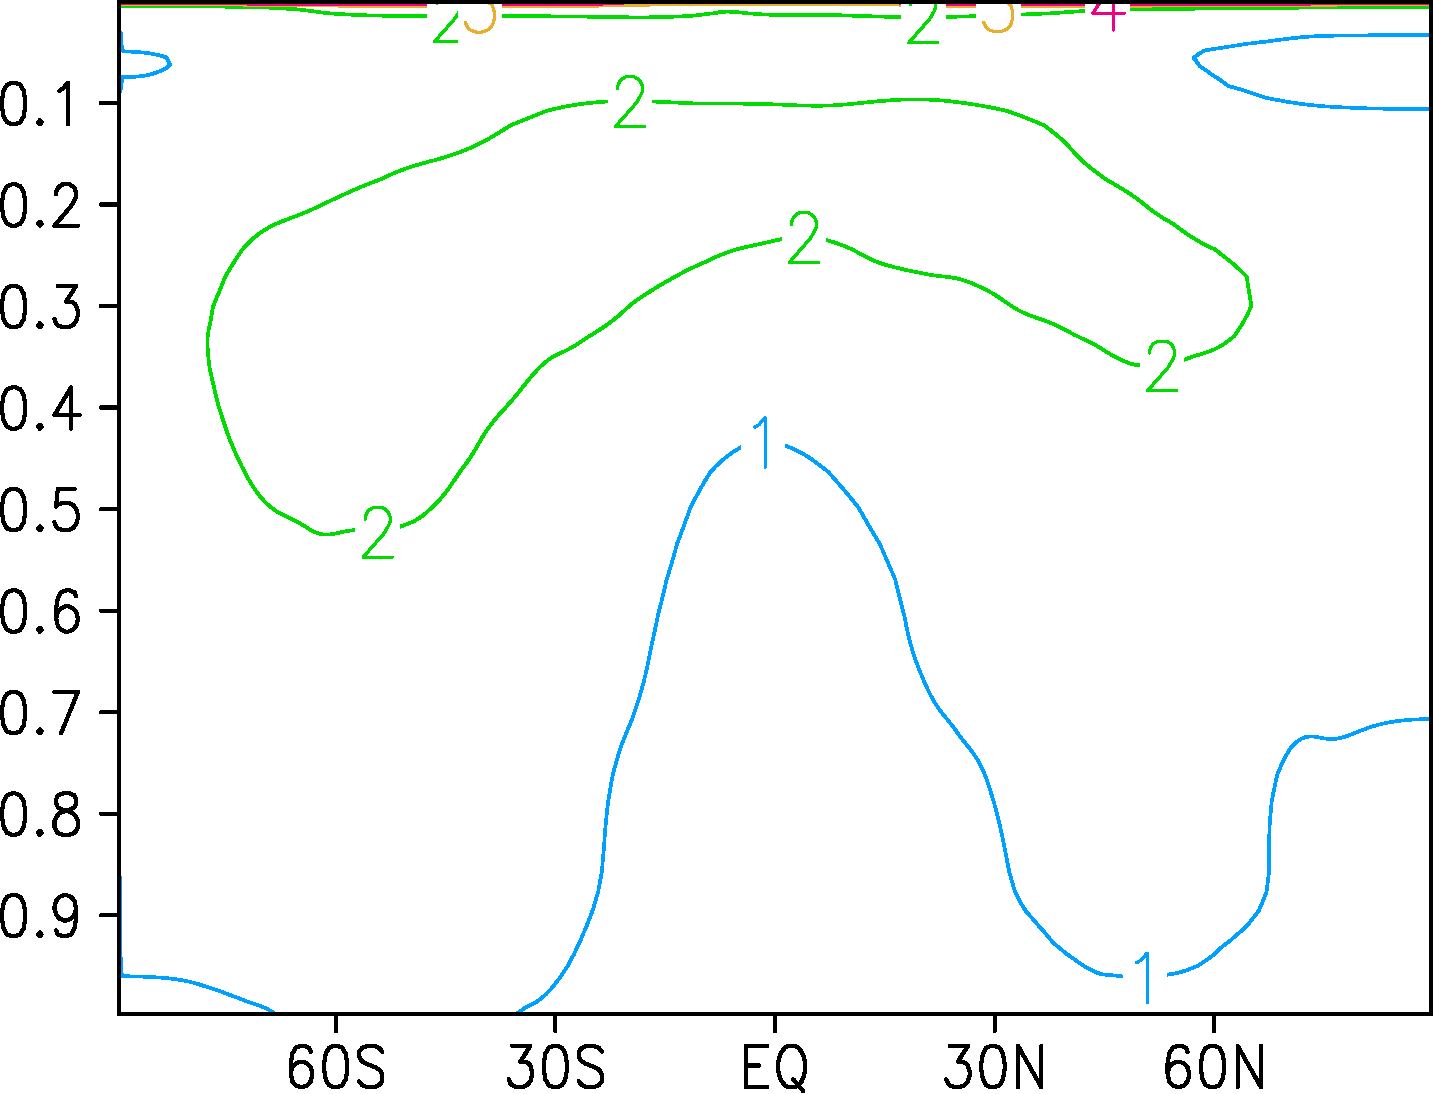
\includegraphics[width=0.3\textwidth,angle=0]{./figs/cap3/amplitudes_novas/amplitudes-NCEP_sf-crop-rotated270.pdf}
        }
        \subfigure[$\mathbf{B}$ CPTEC (00Z), $\psi$]{
          \label{fig:bcptec_00z_psi}
          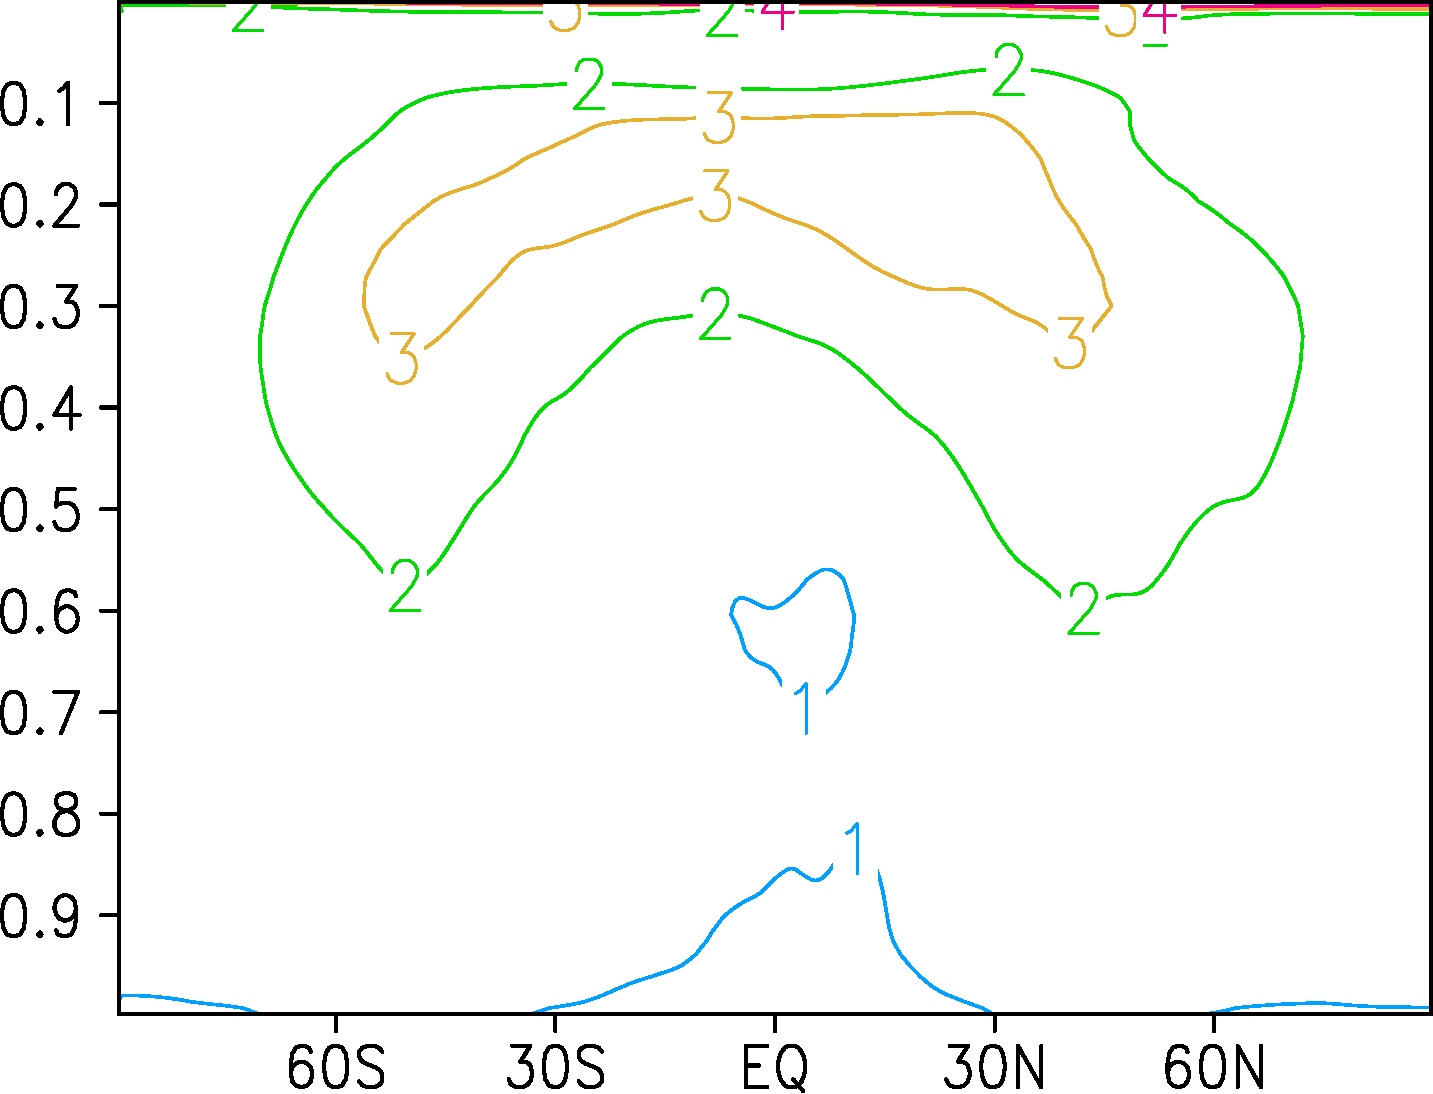
\includegraphics[width=0.3\textwidth,angle=0]{./figs/cap3/amplitudes_novas/amplitudes-B00Z_sf-crop-rotated270.pdf}          
        } 
        \subfigure[$\mathbf{B}$ CPTEC (06Z), $\psi$]{
          \label{fig:bcptec_06z_psi}
          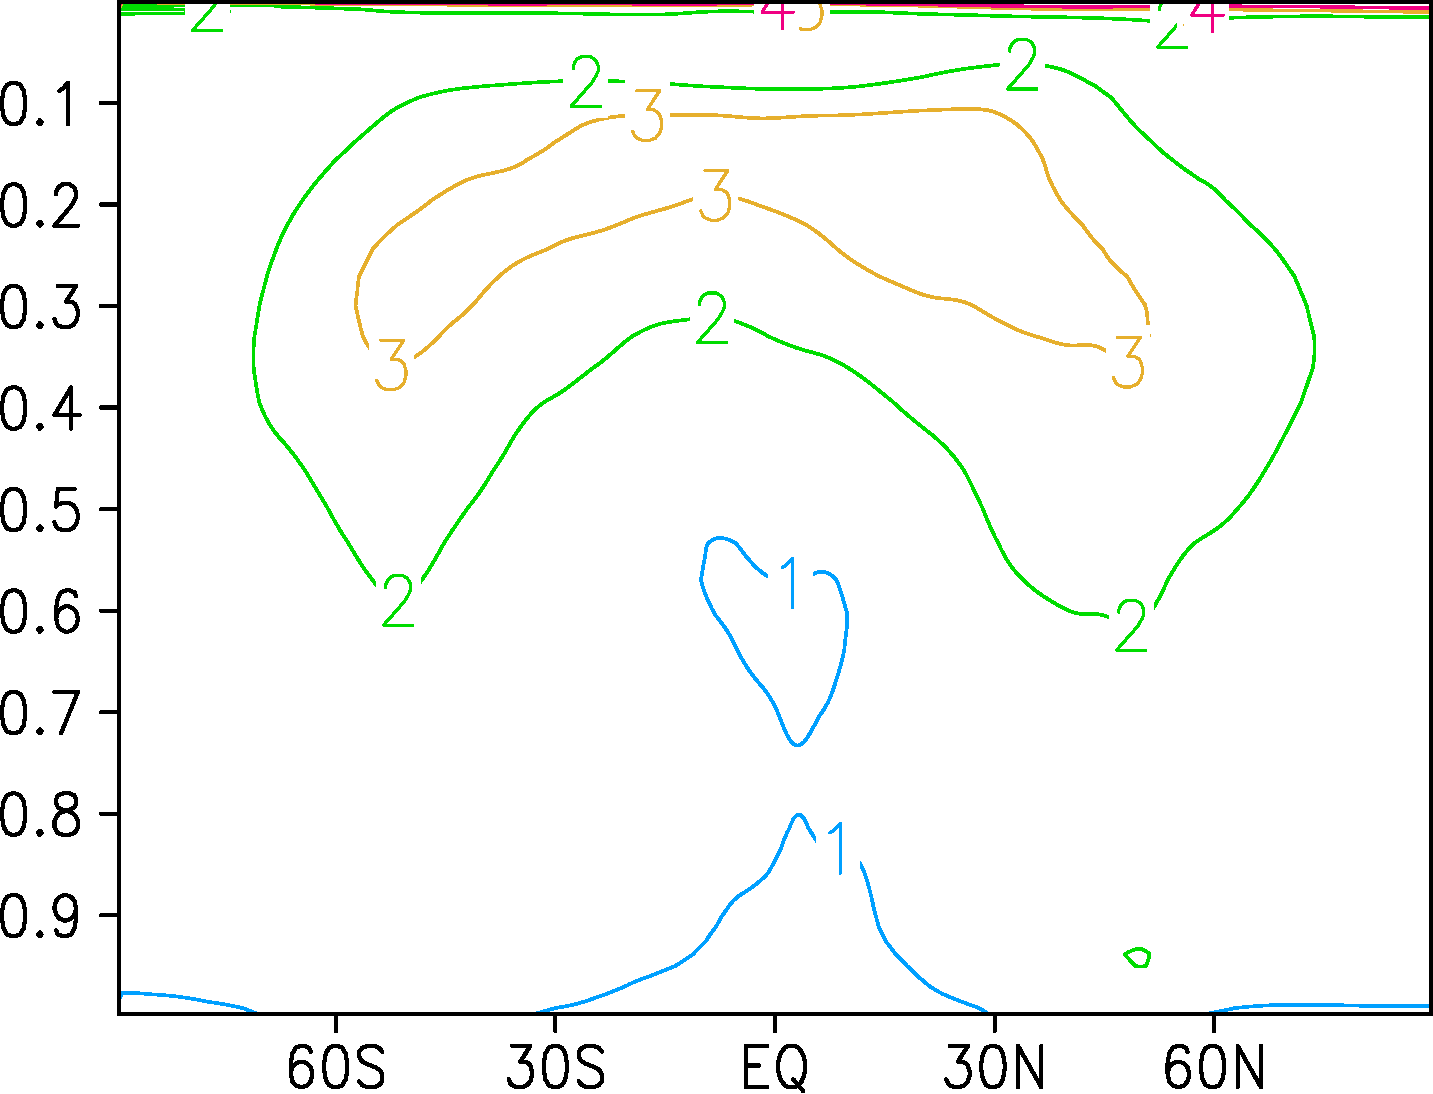
\includegraphics[width=0.3\textwidth,angle=0]{./figs/cap3/amplitudes_novas/amplitudes-B06Z_sf-crop-rotated270.pdf}
        } \\
        \subfigure[$\mathbf{B}$ CPTEC (ALLZ), $\psi$]{
          \label{fig:bcptec_allz_psi}
          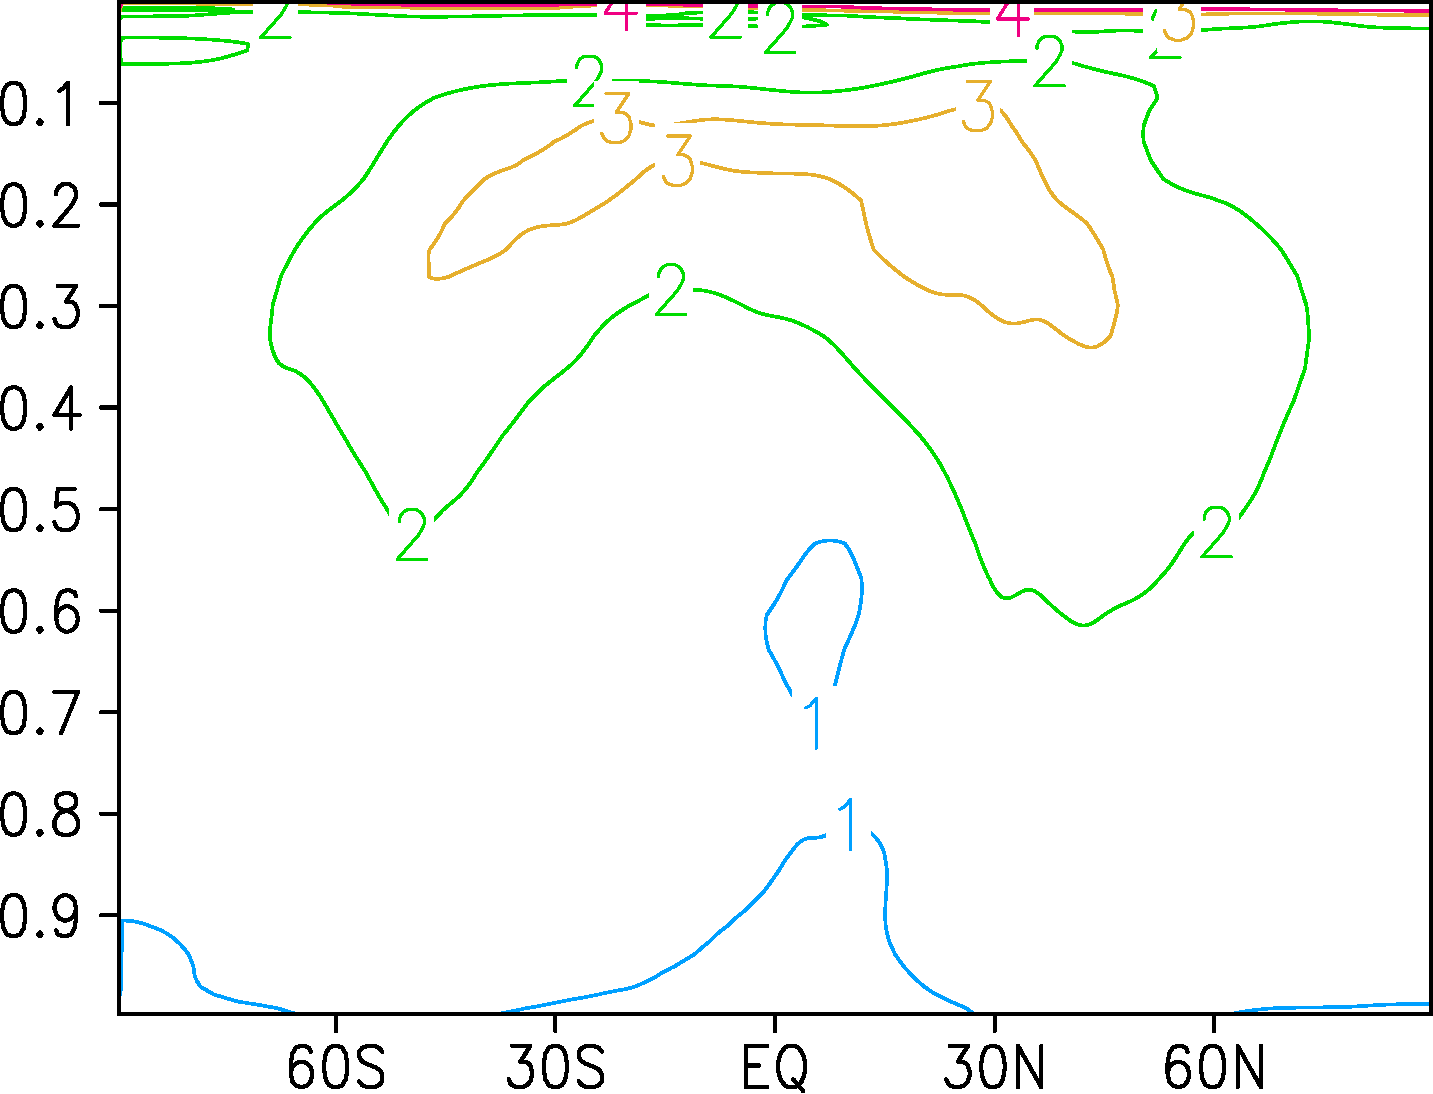
\includegraphics[width=0.3\textwidth,angle=0]{./figs/cap3/amplitudes_novas/amplitudes-BAllZ_sf-crop-rotated270.pdf}
        }   
        \subfigure[$\mathbf{B}$ CPTEC (12Z), $\psi$]{
          \label{fig:bcptec_12z_psi}
          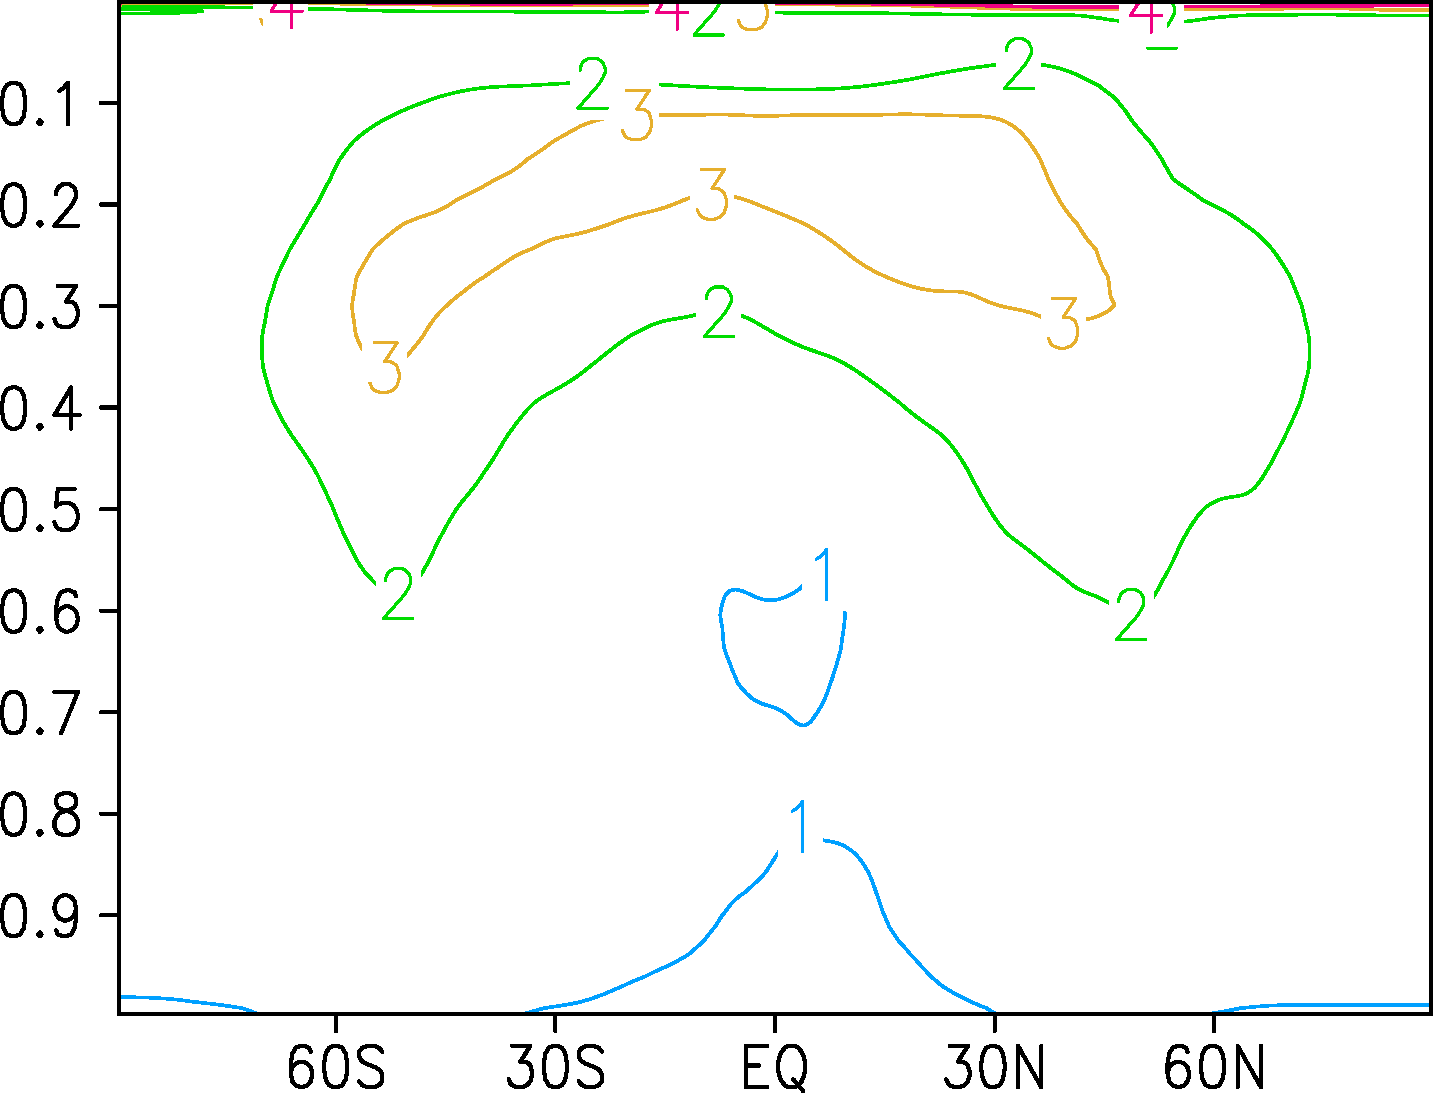
\includegraphics[width=0.3\textwidth,angle=0]{./figs/cap3/amplitudes_novas/amplitudes-B12Z_sf-crop-rotated270.pdf}
        }    
        \subfigure[$\mathbf{B}$ CPTEC (18Z), $\psi$]{
          \label{fig:bcptec_18z_psi}
          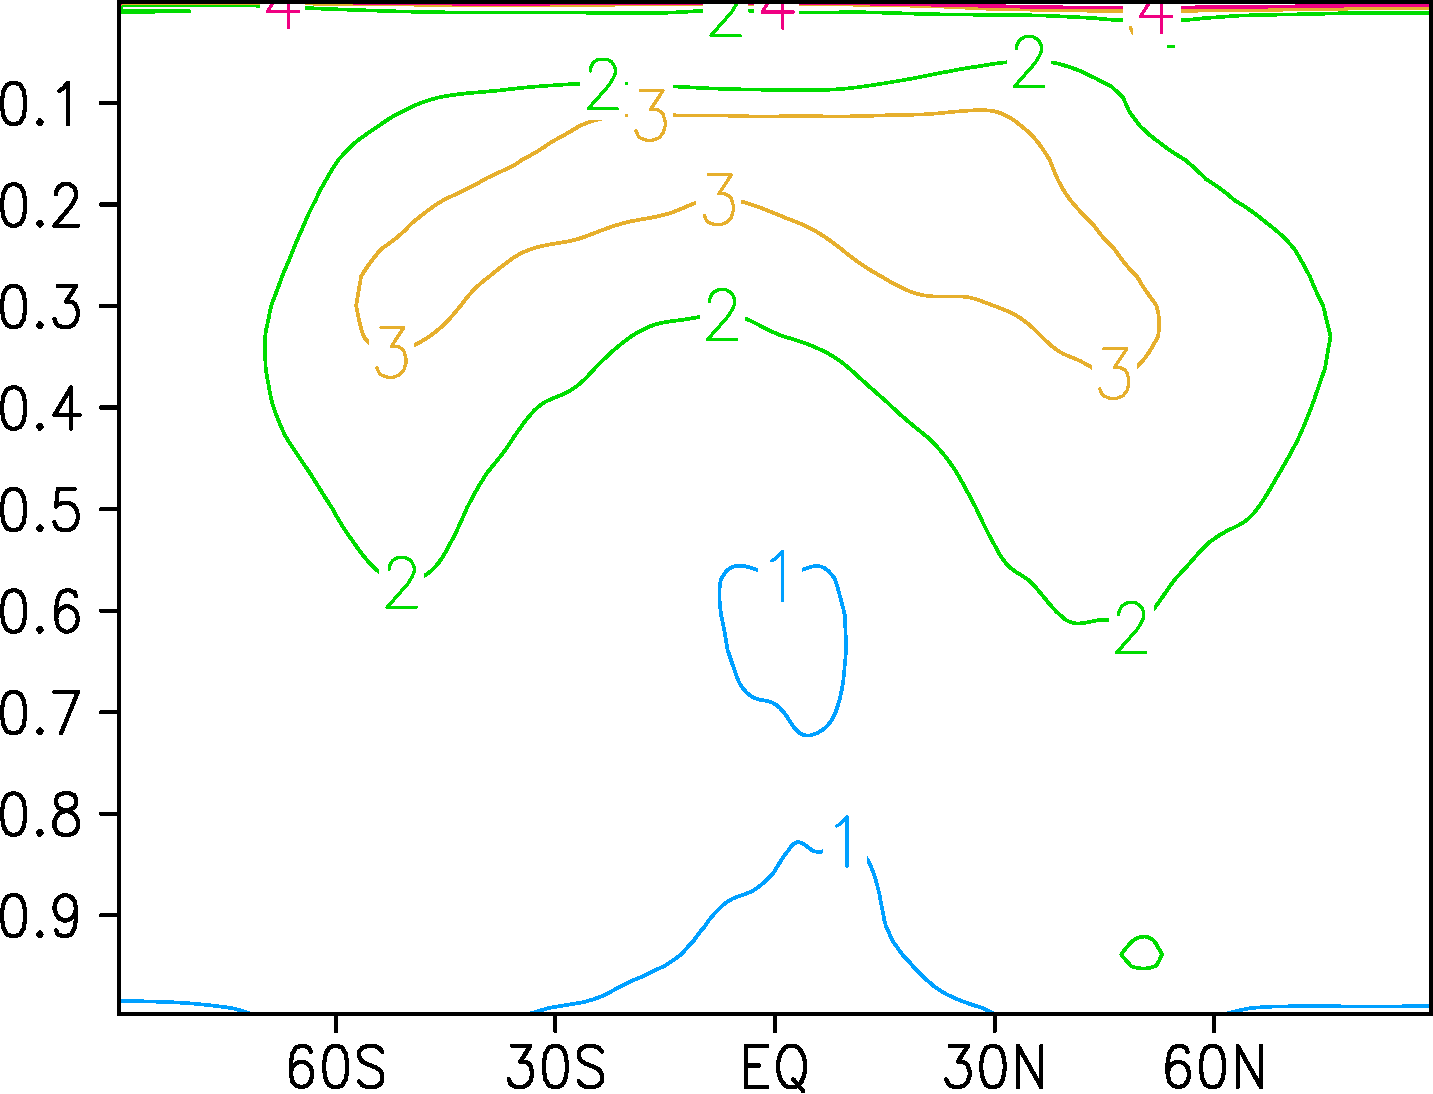
\includegraphics[width=0.3\textwidth,angle=0]{./figs/cap3/amplitudes_novas/amplitudes-B18Z_sf-crop-rotated270.pdf}
        }   
    \end{center}
    \vspace{2mm}
    \legenda{Amplitudes da função de corrente ($\psi$, x $10^{-6}$) ao longo das latitudes e níveis sigma, calculadas utilizando-se o método NMC para todos os horários sinóticos e todos os horários separados. A comparação é feita com o NCEP.}
    \label{fig:B_mcgav4_psi}
    \FONTE{Produção do autor.}
\end{figure}

A Figura \ref{fig:B_mcgav4_psi} mostra a distribuição vertical e latitudinal das amplitudes (variâncias/desvios-padrão) da função de corrente provenientes da matriz de covariâncias do NCEP e do CPTEC. Comparando-se as Figuras \ref{fig:bncep_allz_psi} e \ref{fig:bcptec_allz_psi} (as duas matrizes contendo os pares de previsões de todos os horários sinóticos padrão), observa-se que a amplitude da função de corrente da matriz do CPTEC é mais concentrada, sendo confinada entre os níveis 0.3 a 0.1 sigma (aproximadamente entre 307.2 e 102.4 hPa). As isolinhas de amplitude da função de corrente da matriz do CPTEC, mostram valores maiores nesta região (3x$10^{-6}$) enquanto que a matriz do NCEP apresenta valores menores na mesma região (2x$10^{-6}$), mas espalhado entre os níveis sigma 0.5 e 0.1 (512 e 102.4). Além disso, pode-se observar também a distribuição da amplitude ao longo das latitudes (90N e 90S); nos trópicos ela é menor, apresentando um padrão em forma de ``sino'' (o qual pode ser melhor observado nas demais matrizes, calculadas com os pares de previsões dos horários sinóticos em separado) e maior nos polos.

Esta distribuição da amplitude (variância) da função de corrente para a matriz do CPTEC calculada utilizando-se todos os pares de previsão, não é exatamente semelhante a matriz correspondente do NCEP e esta comparação mostra que, de forma geral, a amplitude da função de corrente no Hemisfério Norte é maior na matriz do CPTEC (o valor em sí é maior e a faixa de latitudes envolvida também), enquanto que esta mesma amplitude é menor no Hemisfério Sul, como representado na matriz de covariâncias do CPTEC. Isto pode estar relacionado a forma como os pares de previsão foram gerados: para o cálculo da matriz de covariâncias do CPTEC, foram utilizados pares de previsões de 48 e 24 horas provenientes do ciclo de assimilação de dados do CPTEC, utilizando-se observações regionalizadas (além daquelas provenientes do \textit{Global Telecomunication System} - GTS). Consequentemente, a variância do erro sobre o Hemisfério Sul, sobretudo sobre a América do Sul (entre 0 e 60S) pode ser menor. Nas outras matrizes do CPTEC (calculadas com os pares exclusivos das 00, 06, 12 e 18Z), observa-se uma distribuição quase simétrica da amplitude da função de corrente, com valores mais próximos da matriz do NCEP, mas com a distribuição, mais localizada ao sul do continente sul-americano.

A Figura \ref{fig:B_mcgav4_chi} mostra a distribuição das amplitudes da velocidade potencial. Assim como para a Figura \ref{fig:B_mcgav4_psi}, as amplitudes calculadas para a velocidade potencial mostram que sobre a região tropical (entre 30S e 30N), a variância do erro na matriz do CPTEC é maior do que a representada pela matriz do NCEP, sobretudo entre os níveis mais baixos do modelo até o nível sigma 0.6 (614 hPa). Comparativamente, cada uma das demais matrizes do CPTEC (00, 06, 12 e 18Z) apresentam similaridades entre si (principalmente entre as matrizes das 00 e 12Z e 06 e 18Z - Figuras \ref{fig:bcptec_00z_chi} e \ref{fig:bcptec_12z_chi}; \ref{fig:bcptec_06z_chi} e \ref{fig:bcptec_18z_chi}, respectivamente).

\begin{figure}[H]
    \vspace{2mm}
    \caption{Idem Figura \ref{fig:B_mcgav4_psi}, para a velocidade potencial ($\chi$ x $10^{-6}$).}
    \begin{center}
        \subfigure[$\mathbf{B}$ NCEP (ALLZ), $\chi$]{
          \label{fig:bncep_allz_chi}
          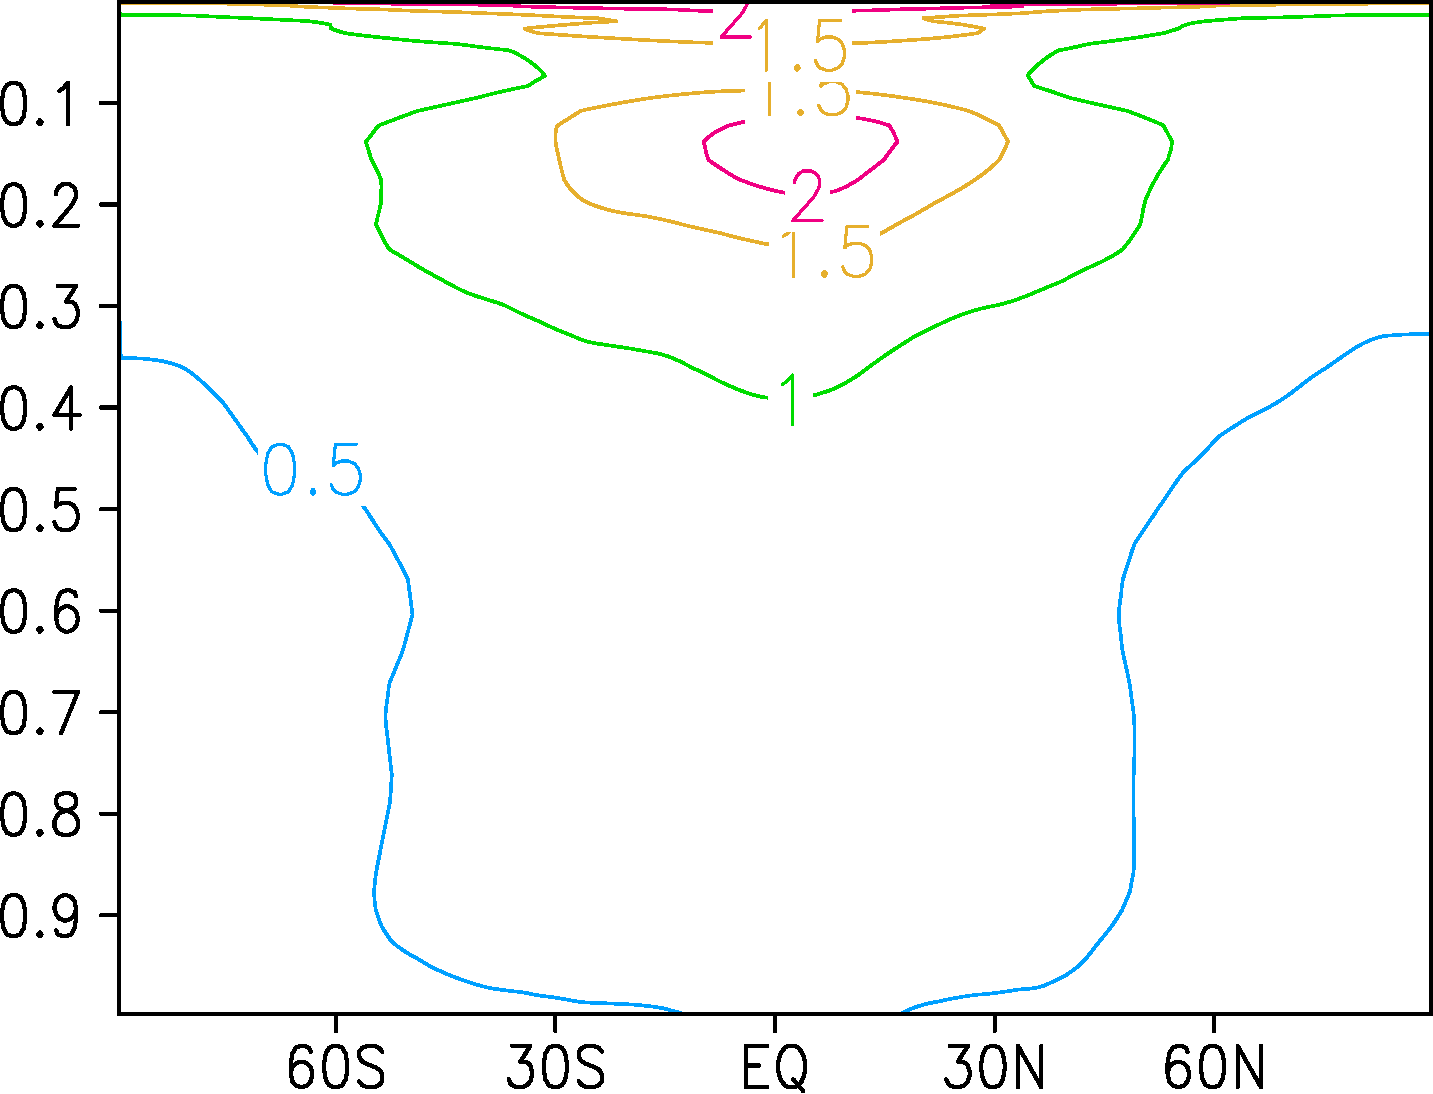
\includegraphics[width=0.3\textwidth,angle=0]{./figs/cap3/amplitudes_novas/amplitudes-NCEP_vp-crop-rotated270.pdf} 
        }
        \subfigure[$\mathbf{B}$ CPTEC (00Z), $\chi$]{
          \label{fig:bcptec_00z_chi}
          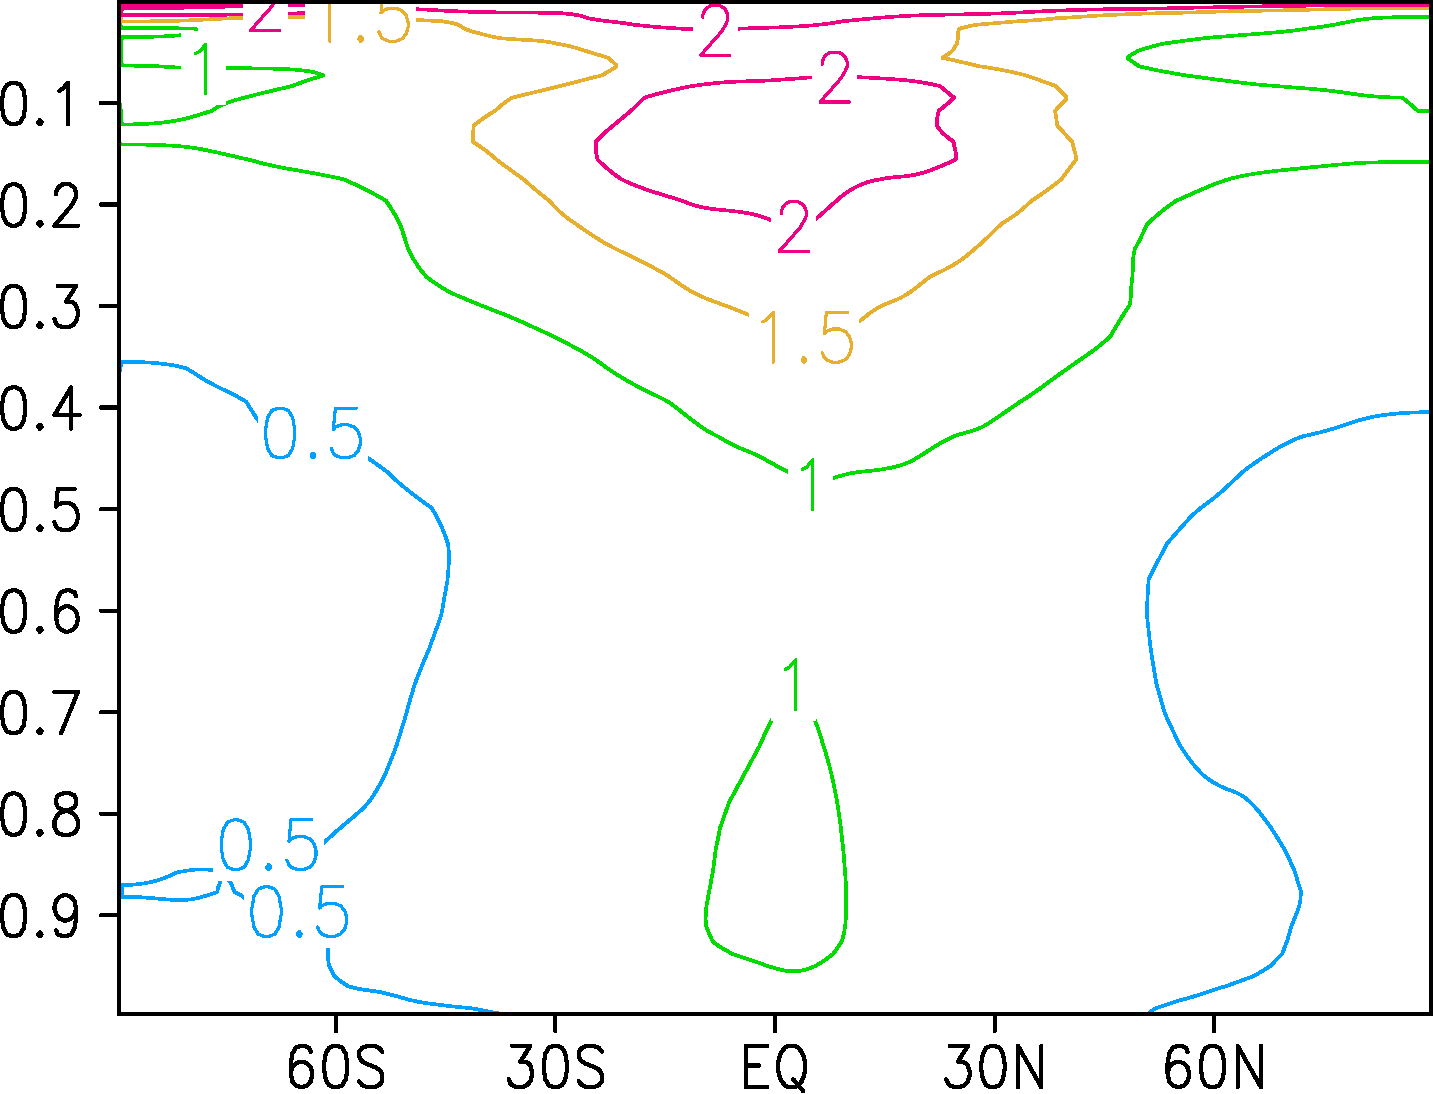
\includegraphics[width=0.3\textwidth,angle=0]{./figs/cap3/amplitudes_novas/amplitudes-B00Z_vp-crop-rotated270.pdf} 
        } 
        \subfigure[$\mathbf{B}$ CPTEC (06Z), $\chi$]{
          \label{fig:bcptec_06z_chi}
          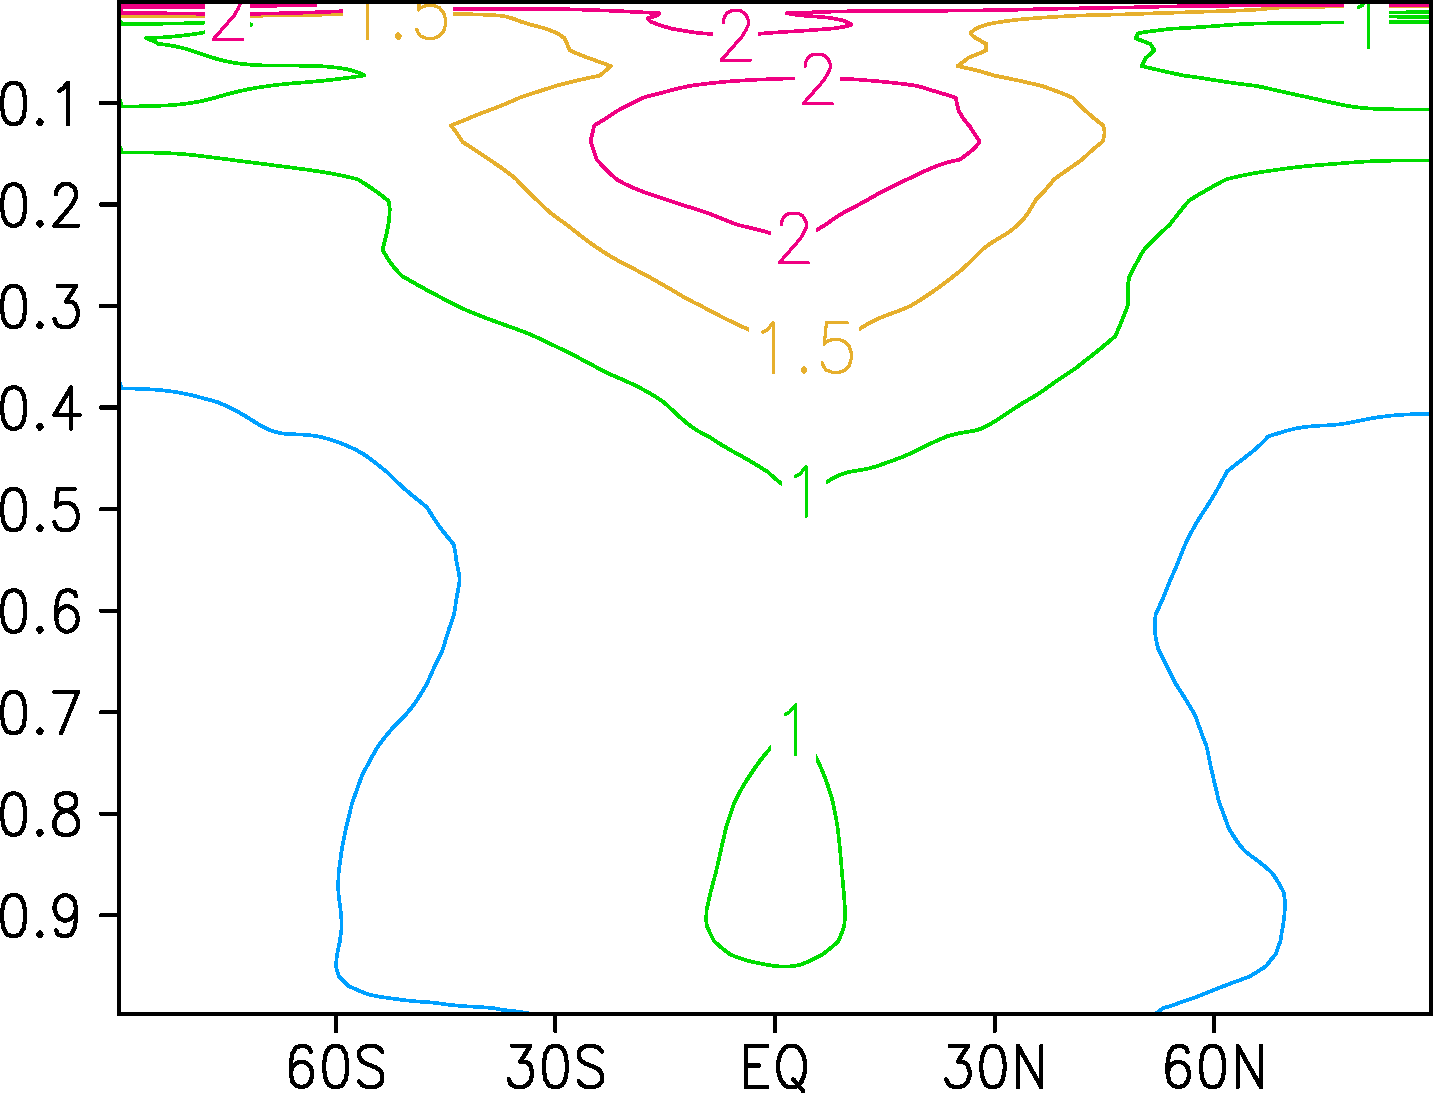
\includegraphics[width=0.3\textwidth,angle=0]{./figs/cap3/amplitudes_novas/amplitudes-B06Z_vp-crop-rotated270.pdf}
        } \\
        \subfigure[$\mathbf{B}$ CPTEC (ALLZ), $\chi$]{
          \label{fig:bcptec_allz_chi}
          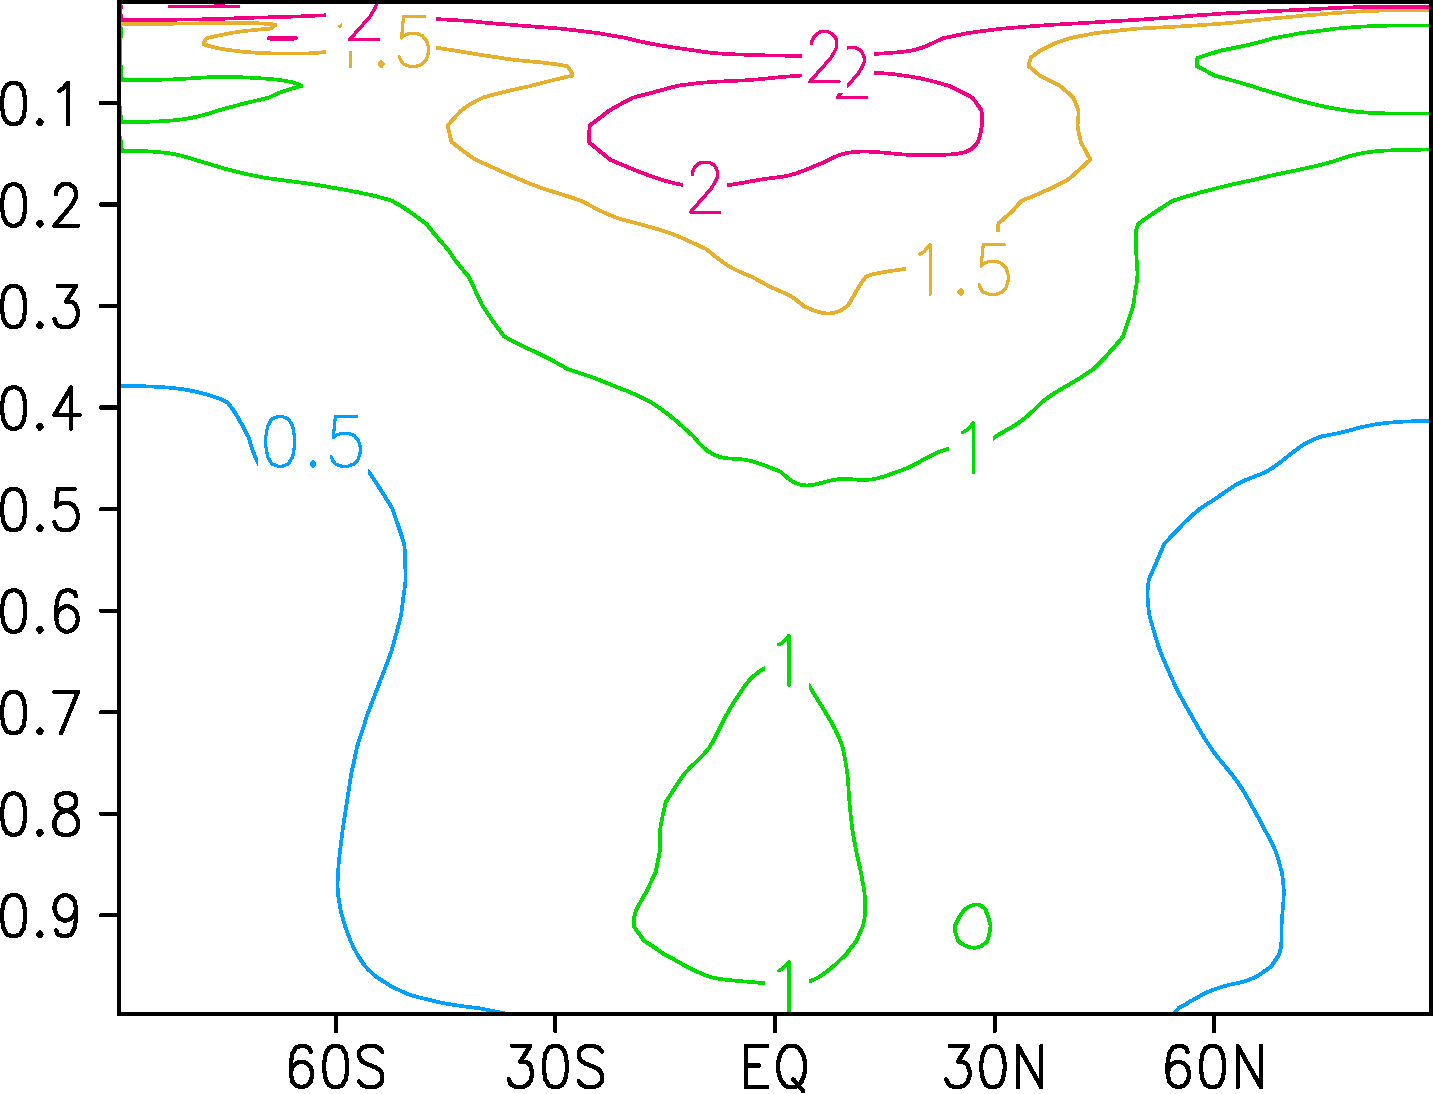
\includegraphics[width=0.3\textwidth,angle=0]{./figs/cap3/amplitudes_novas/amplitudes-BAllZ_vp-crop-rotated270.pdf}
        }   
        \subfigure[$\mathbf{B}$ CPTEC (12Z), $\chi$]{
          \label{fig:bcptec_12z_chi}
          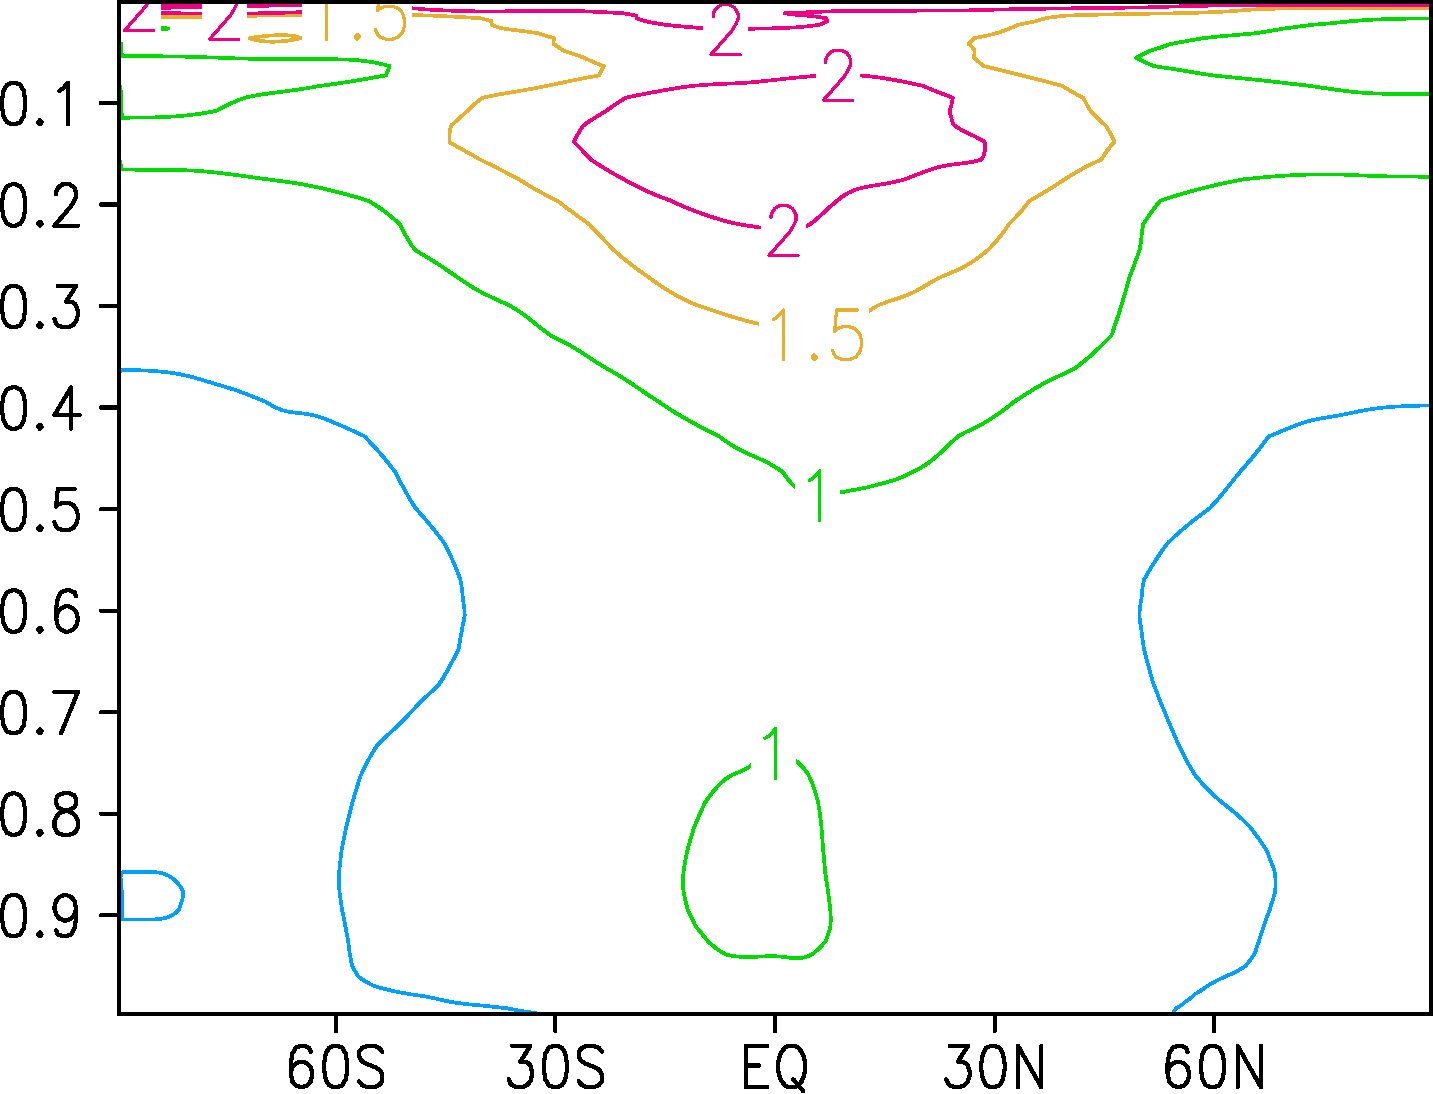
\includegraphics[width=0.3\textwidth,angle=0]{./figs/cap3/amplitudes_novas/amplitudes-B12Z_vp-crop-rotated270.pdf}
        }    
        \subfigure[$\mathbf{B}$ CPTEC (18Z), $\chi$]{
          \label{fig:bcptec_18z_chi}
          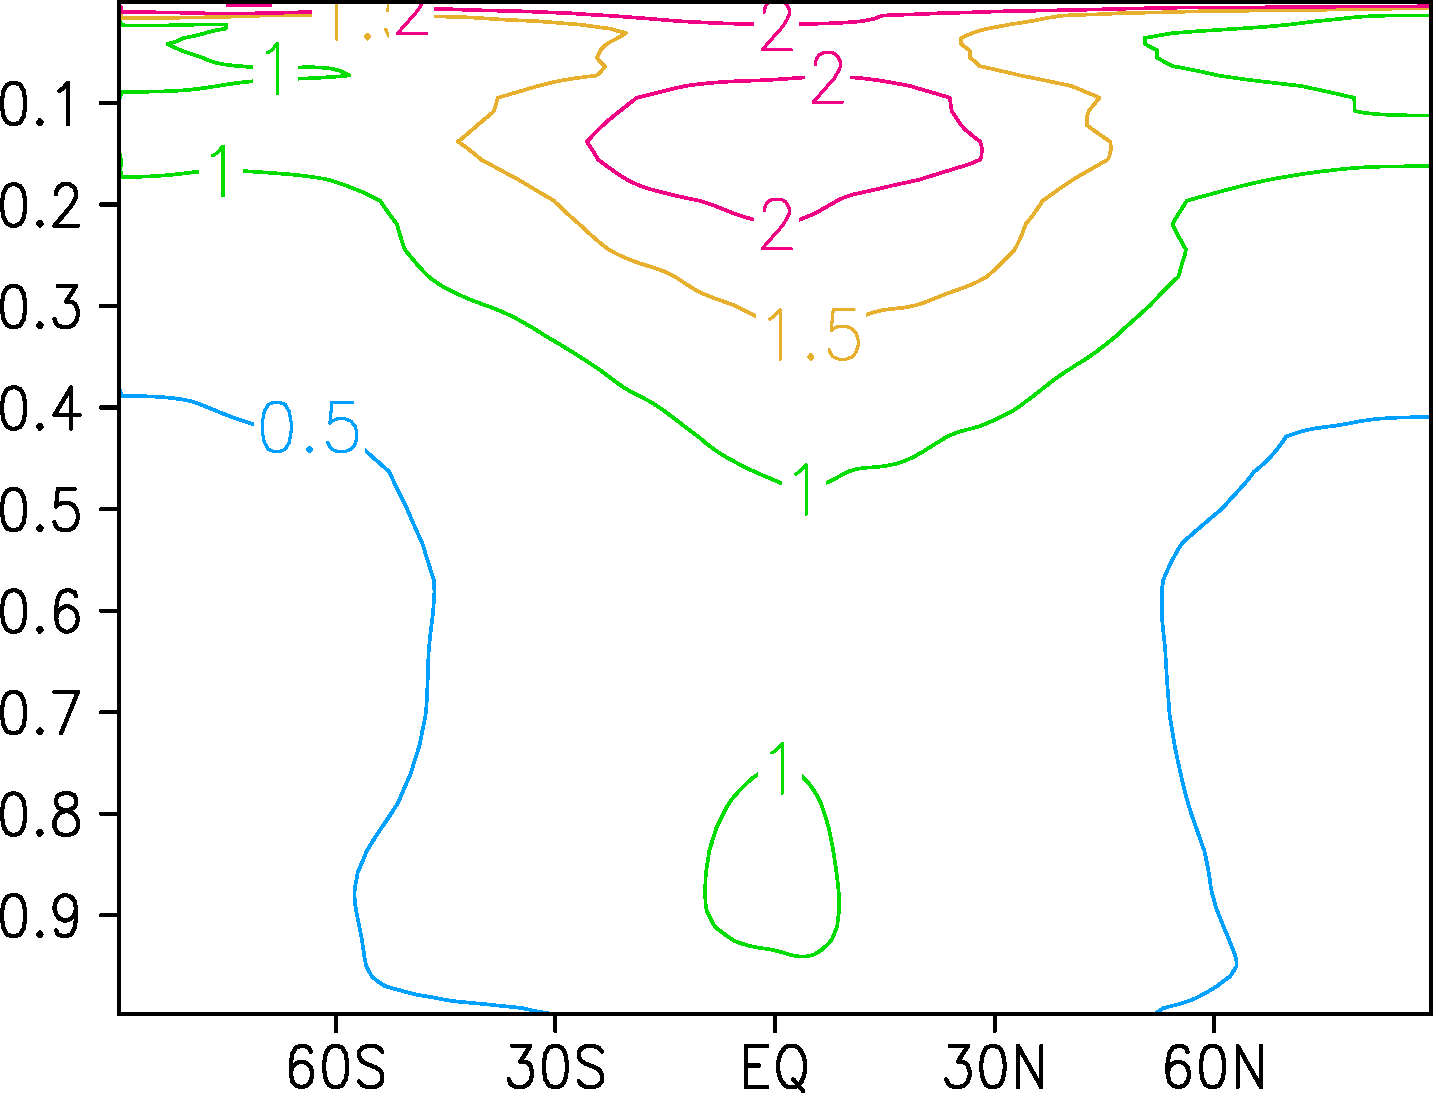
\includegraphics[width=0.3\textwidth,angle=0]{./figs/cap3/amplitudes_novas/amplitudes-B18Z_vp-crop-rotated270.pdf}
        }   
    \end{center}
  \vspace{2mm}
  \legenda{}
  \label{fig:B_mcgav4_chi}
  \FONTE{Produção do autor.}
\end{figure}

A Figura \ref{fig:B_mcgav4_T} a seguir, apresenta a distribuição das amplitudes da temperatura, sendo que estes valores na matriz do CPTEC completa (i.e., BAllZ - Figura \ref{fig:bcptec_00z_t}), onde a maior parte da variância encontra-se concentrada sobre o Hemisfério Norte, mais precisamente a partir de 30N (isolinha de 1 na Figura \ref{fig:bcptec_00z_t}); esta mesma isolinha na matriz do NCEP (Figura \ref{fig:bncep_allz_t}) está desenhada a partir de aproximadamente 45N. Em ambas as matrizes, esta amplitude é limitada as primeiras camadas do modelo (ie., entre a superfície e o nível sigma de 0.8 ou 819.2 hPa). Nas demais matrizes, observa-se um padrão semelhante em relação a distribuição das amplitudes, sendo que no Hemisfério Norte, estas alcançam os 819.2 hPa, enquanto que no Hemisfério Sul, não ultrapassam este nível.


\begin{figure}[H]
    \vspace{2mm}
    \caption{Idem Figura \ref{fig:B_mcgav4_psi}, para a temperatura ($T$).}
    \begin{center}
        \subfigure[$\mathbf{B}$ NCEP (ALLZ), $T$]{
          \label{fig:bncep_allz_t}
          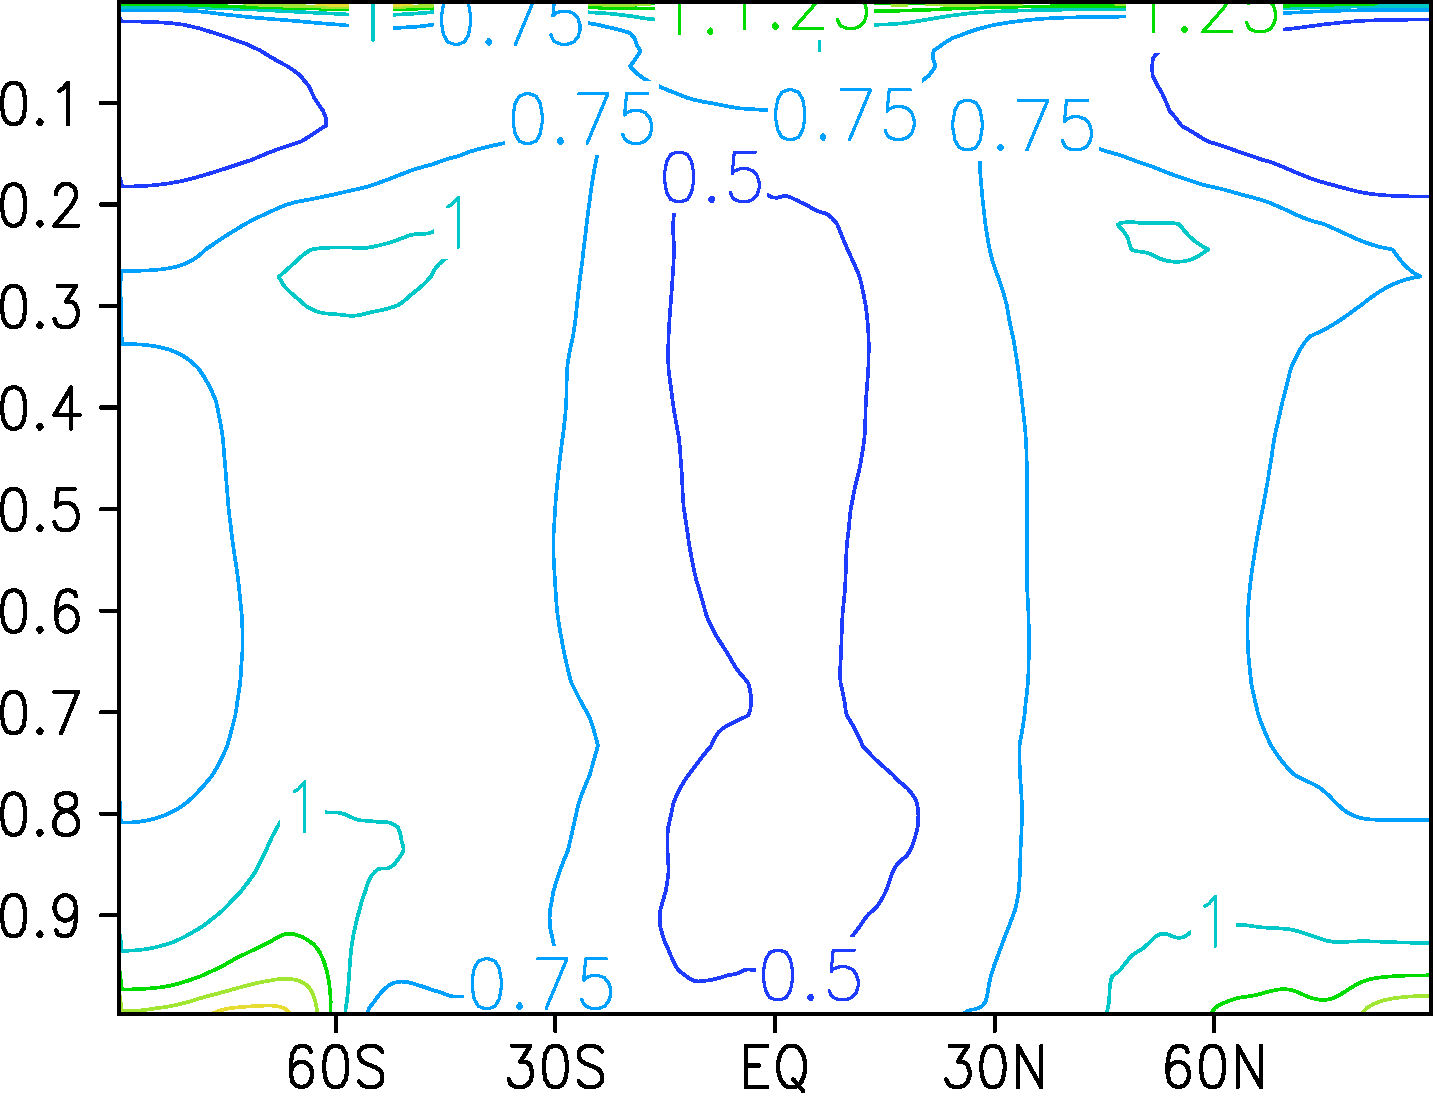
\includegraphics[width=0.3\textwidth,angle=0]{./figs/cap3/amplitudes_novas/amplitudes-NCEP_t-crop-rotated270.pdf} 
        }
        \subfigure[$\mathbf{B}$ CPTEC (00Z), $T$]{
          \label{fig:bcptec_00z_t}
          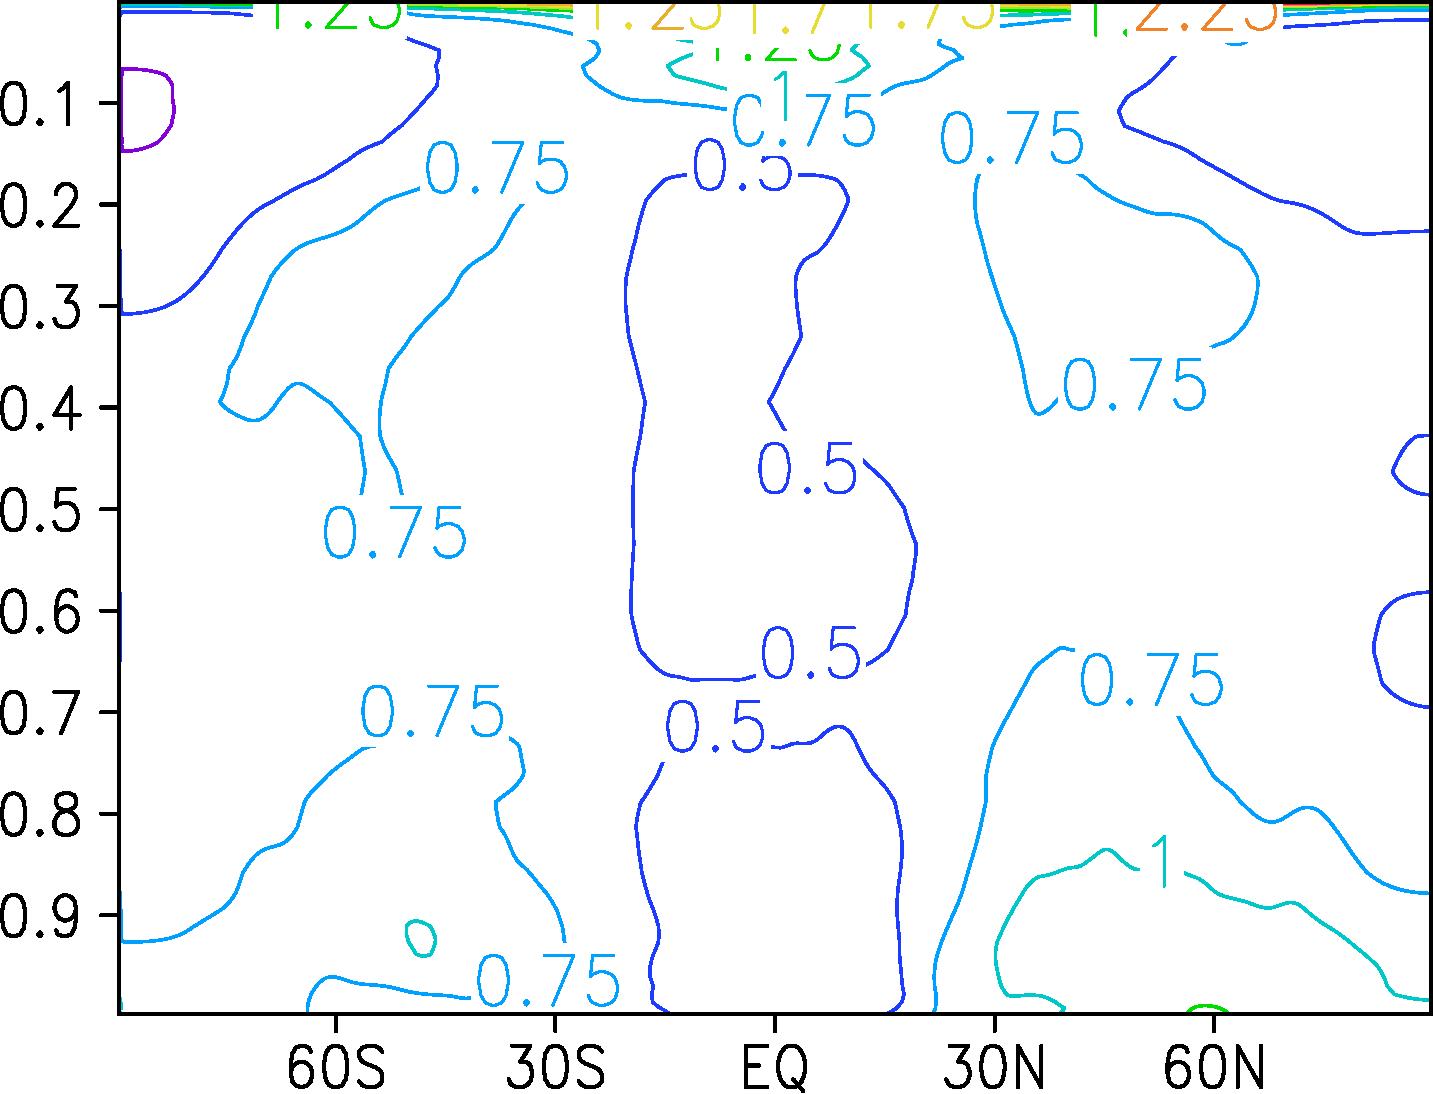
\includegraphics[width=0.3\textwidth,angle=0]{./figs/cap3/amplitudes_novas/amplitudes-B00Z_t-crop-rotated270.pdf}
        } 
        \subfigure[$\mathbf{B}$ CPTEC (06Z), $T$]{
          \label{fig:bcptec_06z_t}
          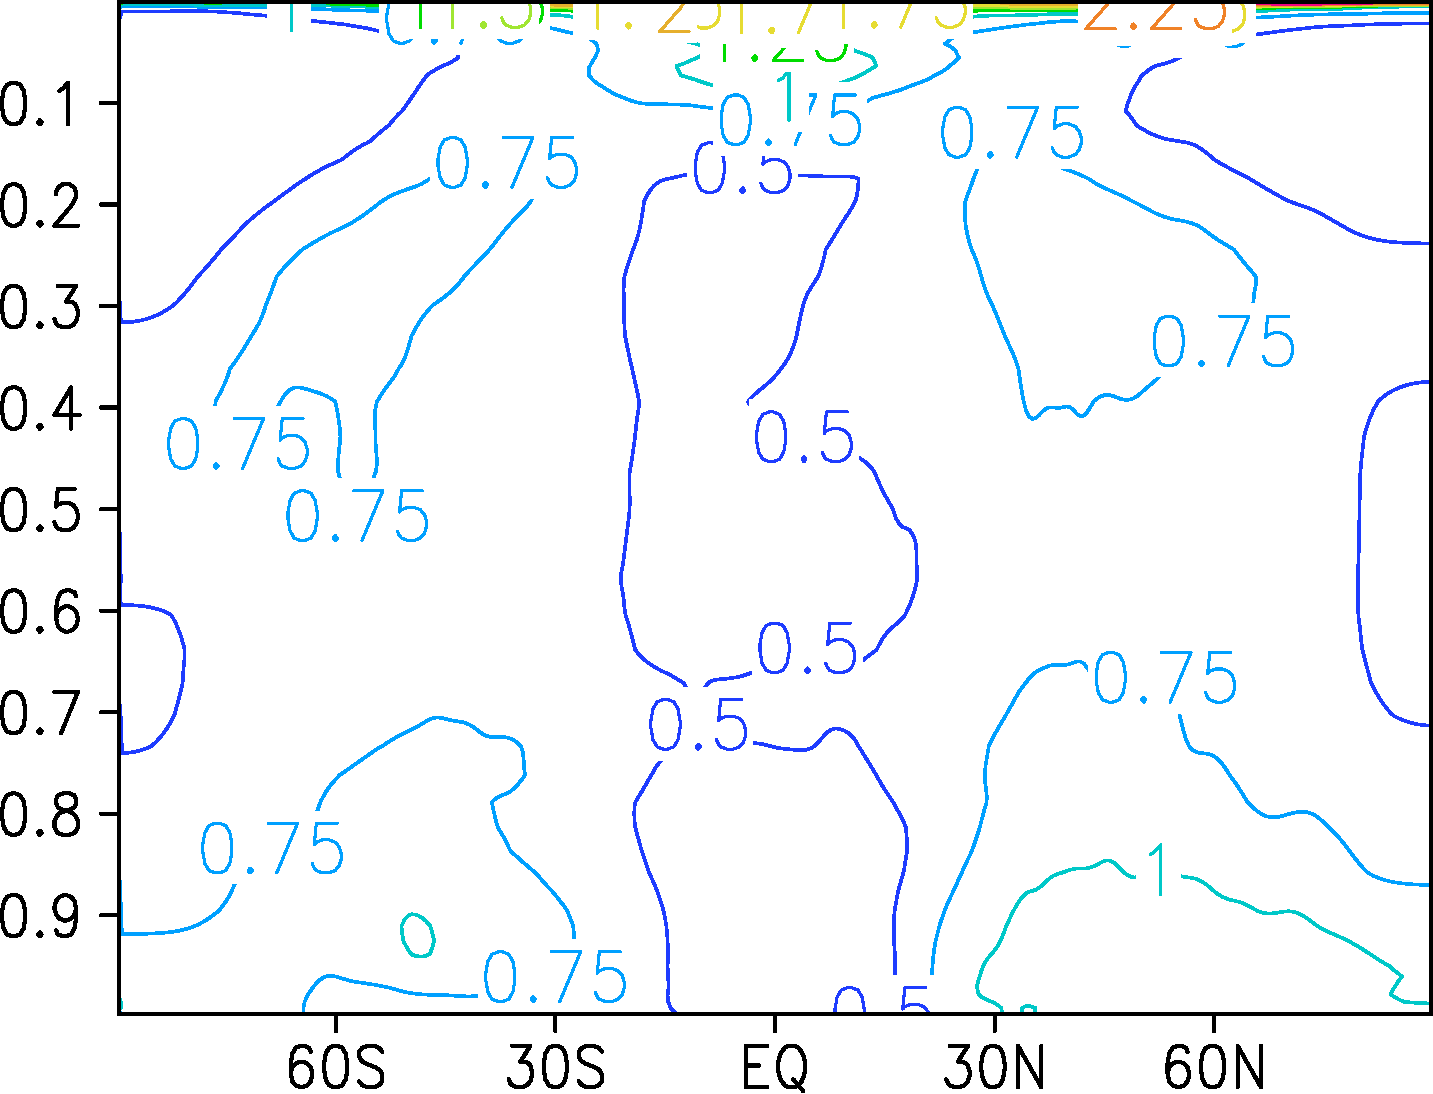
\includegraphics[width=0.3\textwidth,angle=0]{./figs/cap3/amplitudes_novas/amplitudes-B06Z_t-crop-rotated270.pdf}
        } \\
        \subfigure[$\mathbf{B}$ CPTEC (ALLZ), $T$]{
          \label{fig:bcptec_allz_t}
          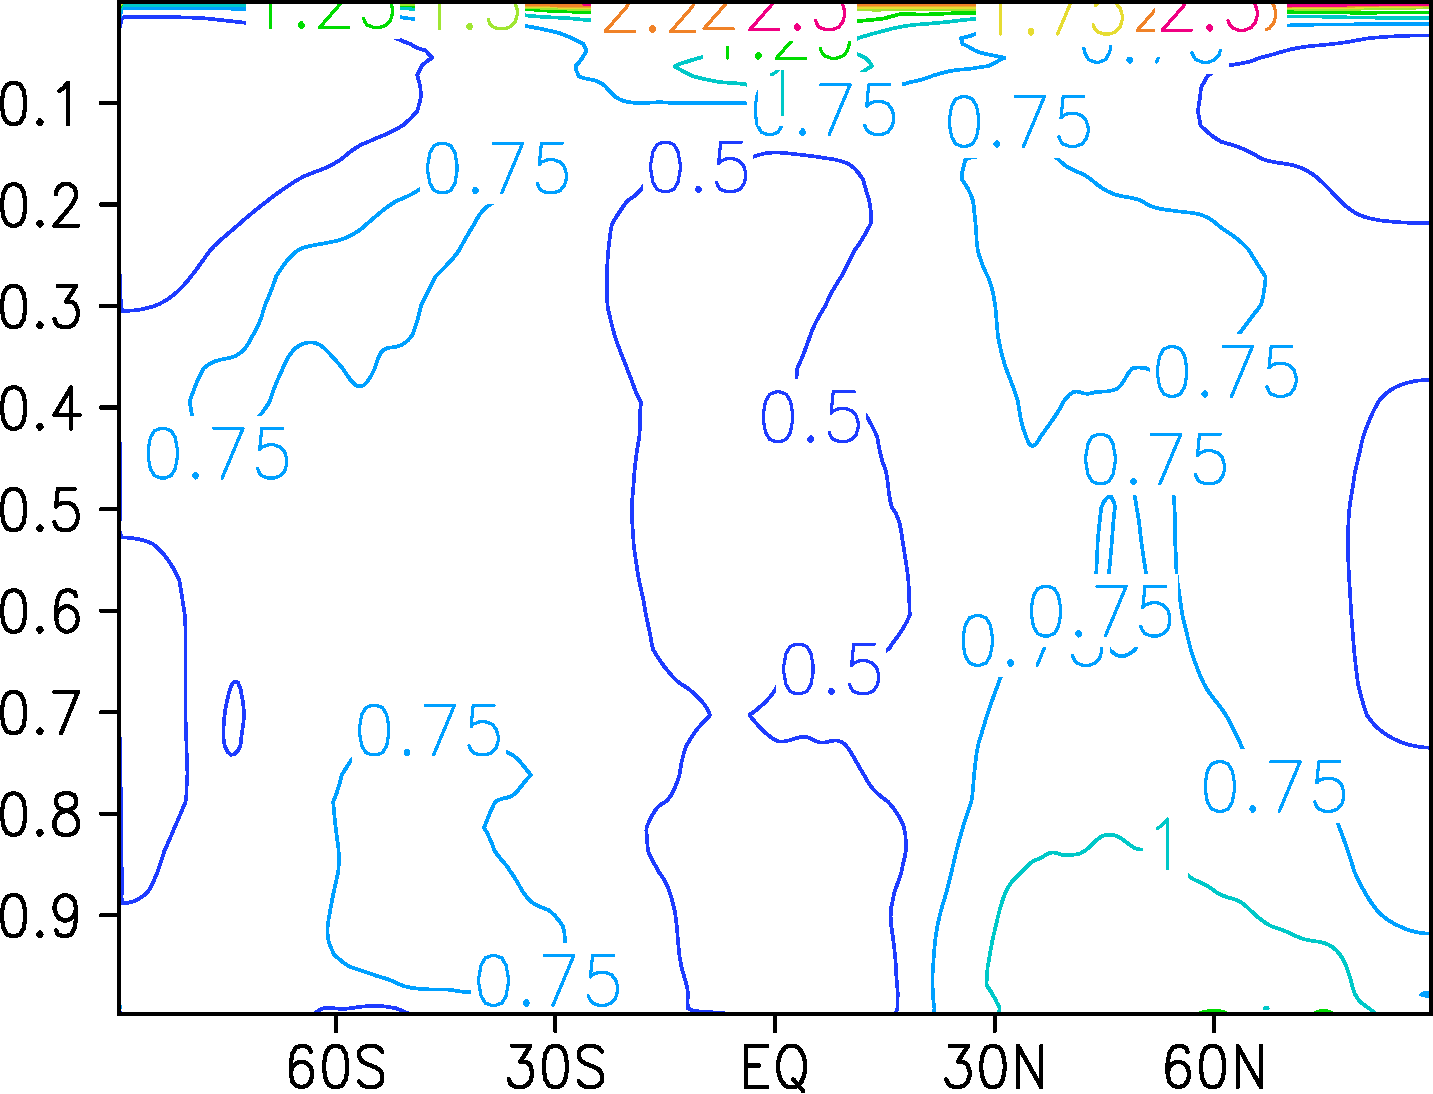
\includegraphics[width=0.3\textwidth,angle=0]{./figs/cap3/amplitudes_novas/amplitudes-BAllZ_t-crop-rotated270.pdf}
        }   
        \subfigure[$\mathbf{B}$ CPTEC (12Z), $T$]{
          \label{fig:bcptec_12z_t}
          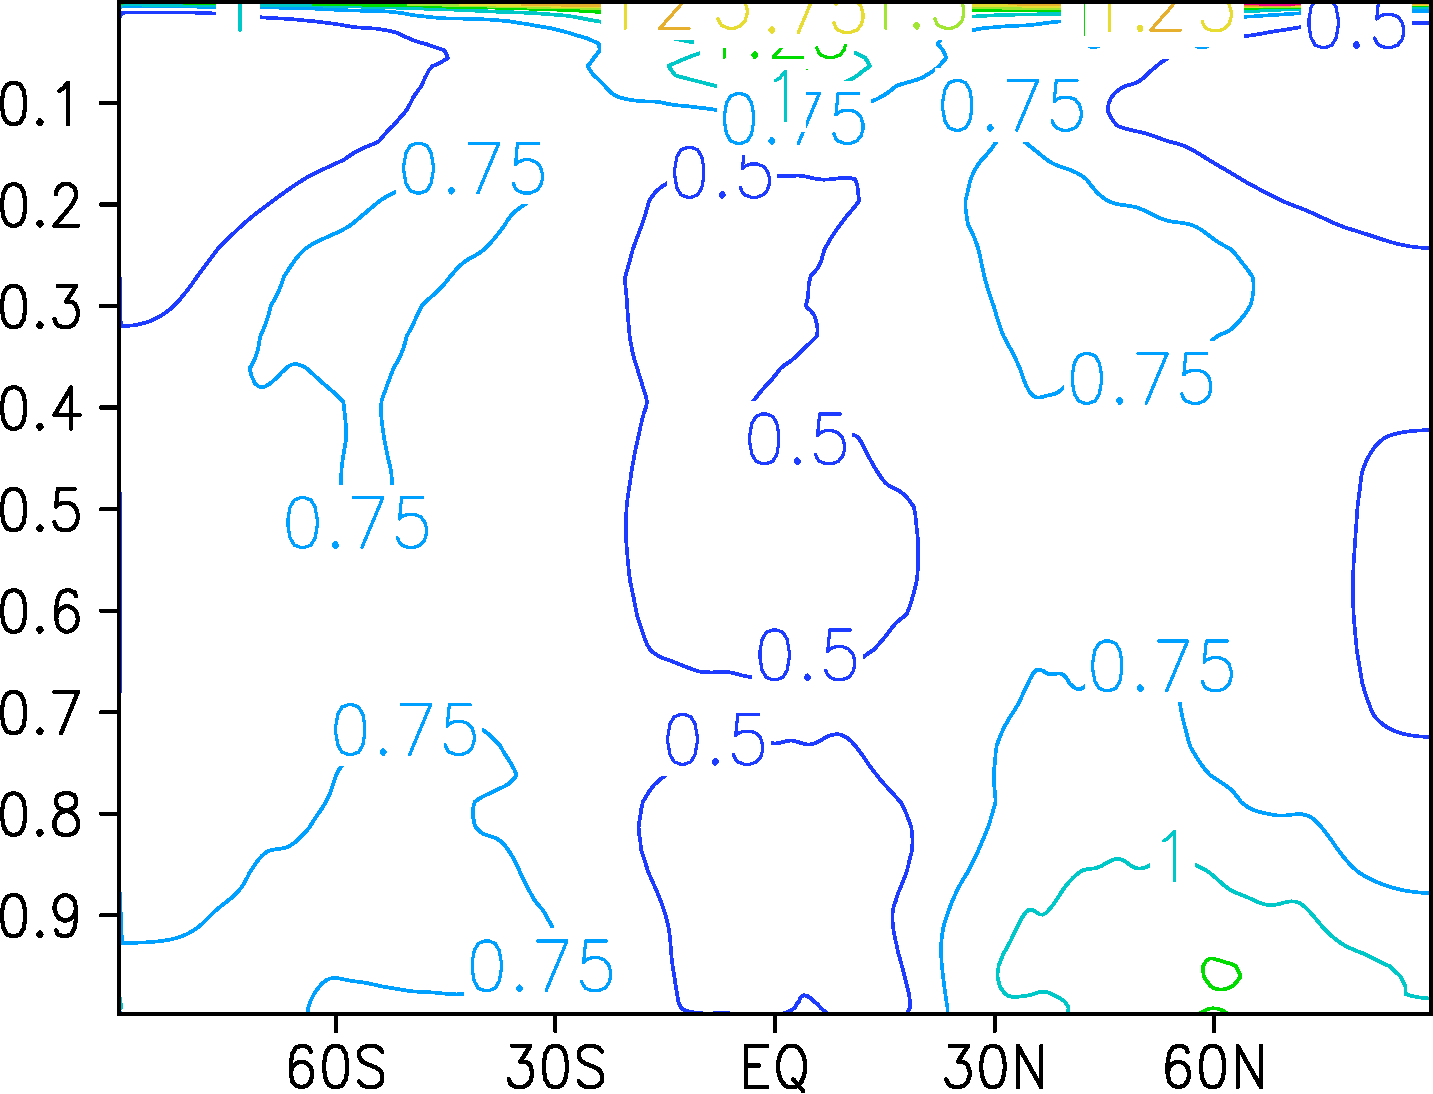
\includegraphics[width=0.3\textwidth,angle=0]{./figs/cap3/amplitudes_novas/amplitudes-B12Z_t-crop-rotated270.pdf}
        }    
        \subfigure[$\mathbf{B}$ CPTEC (18Z), $T$]{
          \label{fig:bcptec_18z_t}
          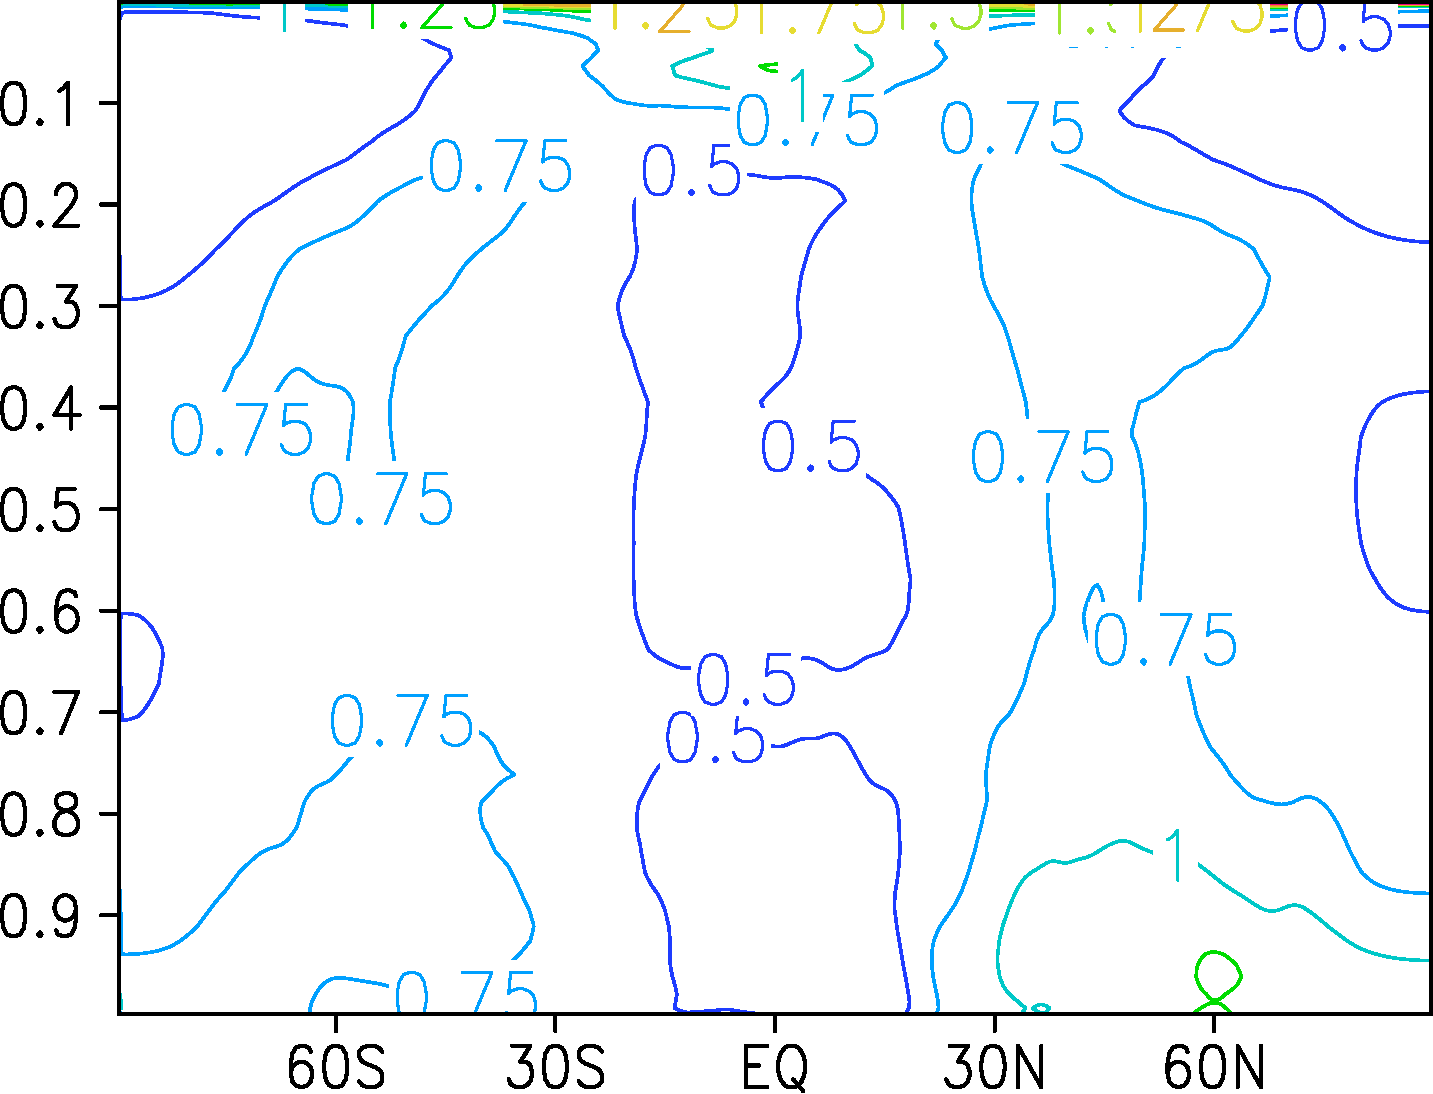
\includegraphics[width=0.3\textwidth,angle=0]{./figs/cap3/amplitudes_novas/amplitudes-B18Z_t-crop-rotated270.pdf}
        }   
  \end{center}
  \vspace{2mm}
  \legenda{}
  \label{fig:B_mcgav4_T}
  \FONTE{Produção do autor.}
\end{figure}

As amplitudes da umidade apresentada na Figura \ref{fig:bcptec_allz_q} para a matriz CPTEC BAllZ, não difere muito em distribuição ao longo das latitudes como nas demais matrizes (i.e., 00, 06, 12 e 18Z - Figuras \ref{fig:bcptec_00z_q}, \ref{fig:bcptec_06z_q}, \ref{fig:bcptec_12z_q} e \ref{fig:bcptec_18z_q}, respectivamente), mas a amplitude da variância nos subtrópicos em ambos os hemisférios (entre 60S e 30S e entre 30N e 60N), é melhor definida e menos intensa também do que aquela representada em B NCEP (Figura \ref{fig:bncep_allz_q}). Neste caso, a variância da umidade em ambos os hemisférios é bastante simétrica, principalmente nos casos calculados com as previsões do CPTEC. Isto pode reforçar a necessidade de se remover o viés do modelo do CPTEC. Neste caso, as isolinhas mais próximas a superfície (até o nível sigma 0.8 ou 819.2 hPa), apresentam valores com quase o dobro do valor, se comparados com a mesma região na matriz do NCEP. De outra forma, pode mostrar também alguma deficiência na física do modelo em representar com melhor precisão os processos úmidos (que dependem da física do modelo).

\begin{figure}[H]
    \vspace{2mm}
    \caption{Idem Figura \ref{fig:B_mcgav4_psi}, para a umidade ($q$).}
    \begin{center}
        \subfigure[$\mathbf{B}$ NCEP (ALLZ), $q$]{
          \label{fig:bncep_allz_q}
          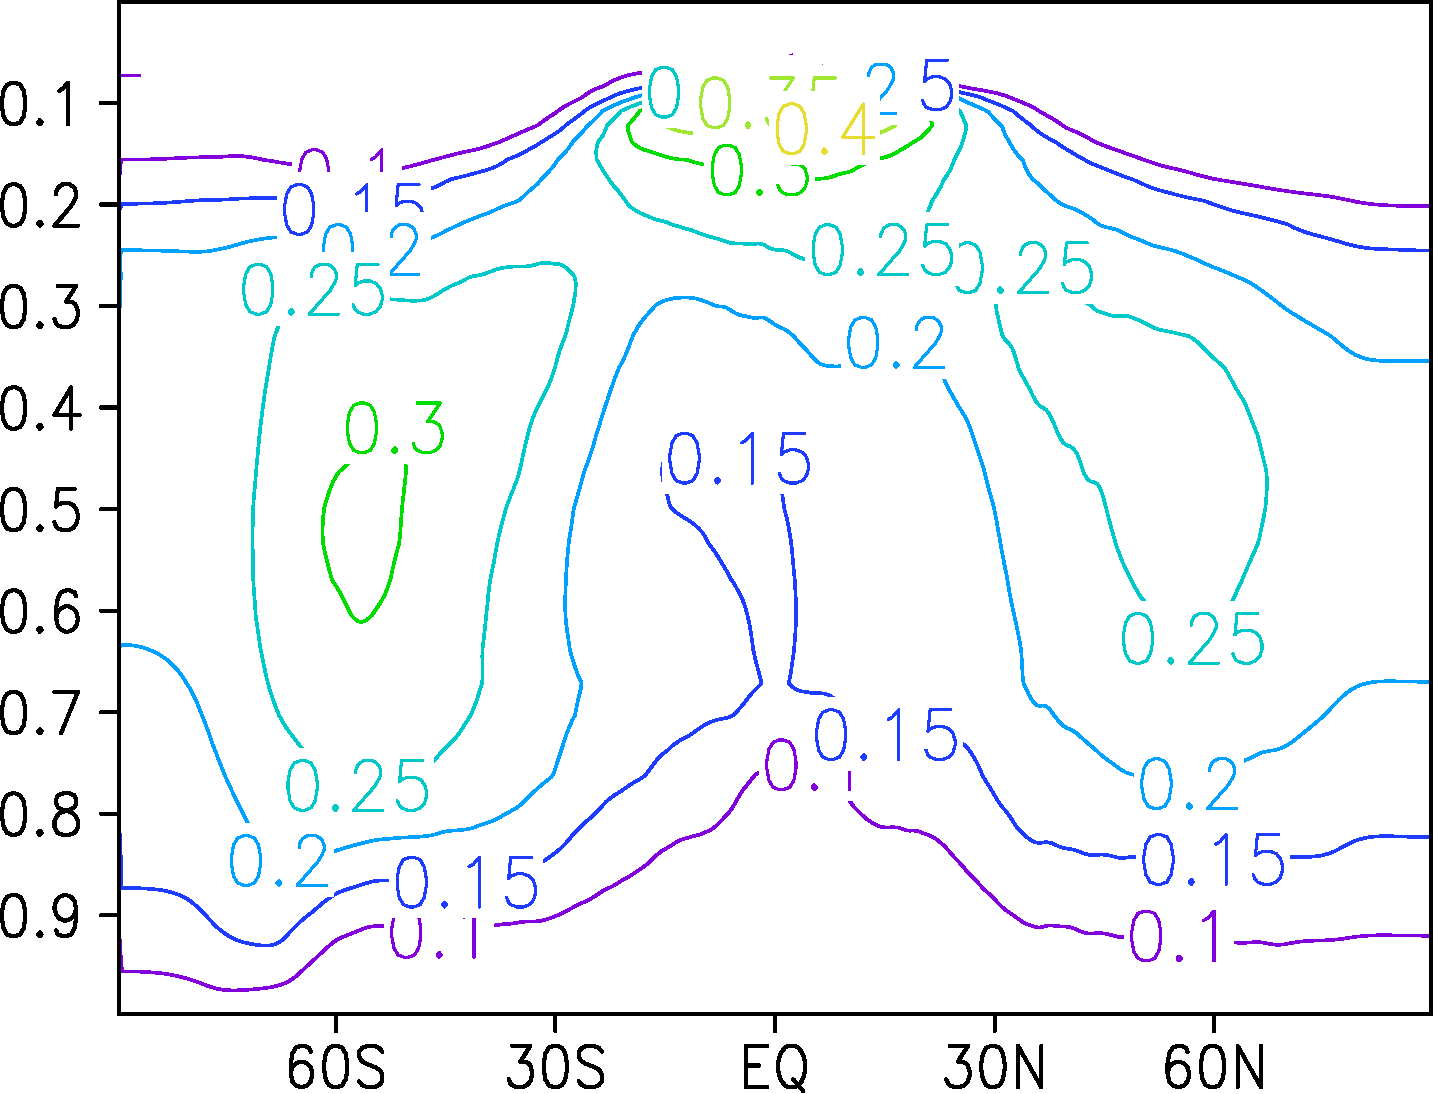
\includegraphics[width=0.3\textwidth,angle=0]{./figs/cap3/amplitudes_novas/amplitudes-NCEP_q-crop-rotated270.pdf} 
        }
        \subfigure[$\mathbf{B}$ CPTEC (00Z), $q$]{
          \label{fig:bcptec_00z_q}
          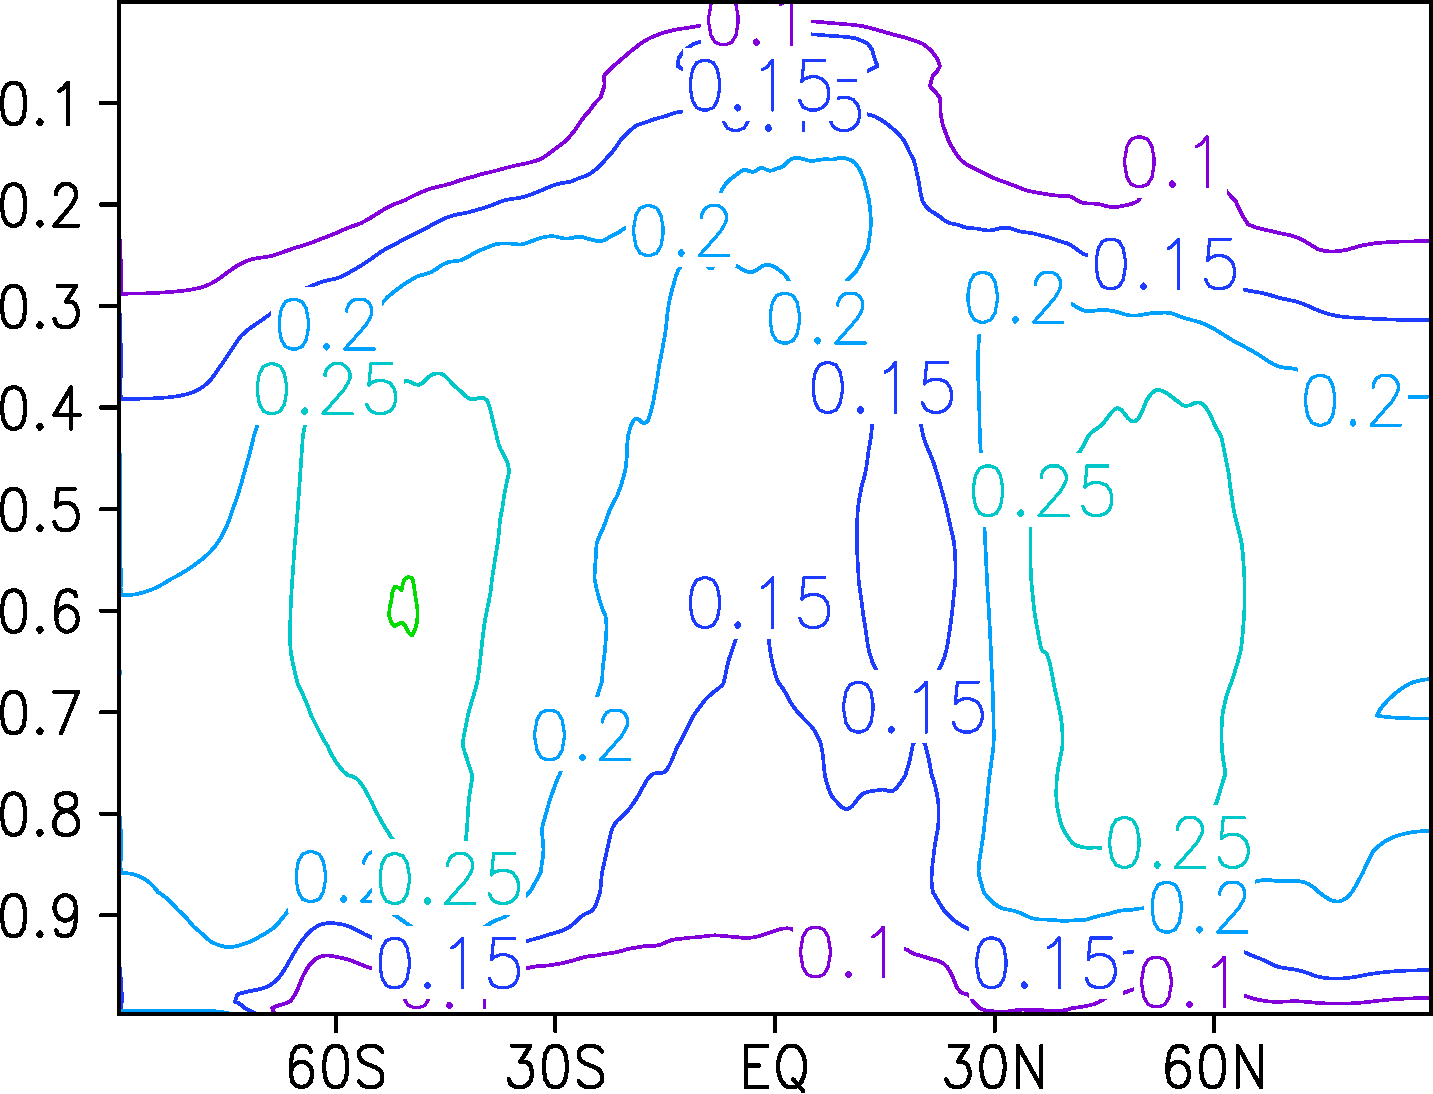
\includegraphics[width=0.3\textwidth,angle=0]{./figs/cap3/amplitudes_novas/amplitudes-B00Z_q-crop-rotated270.pdf}
        } 
        \subfigure[$\mathbf{B}$ CPTEC (06Z), $q$]{
          \label{fig:bcptec_06z_q}
          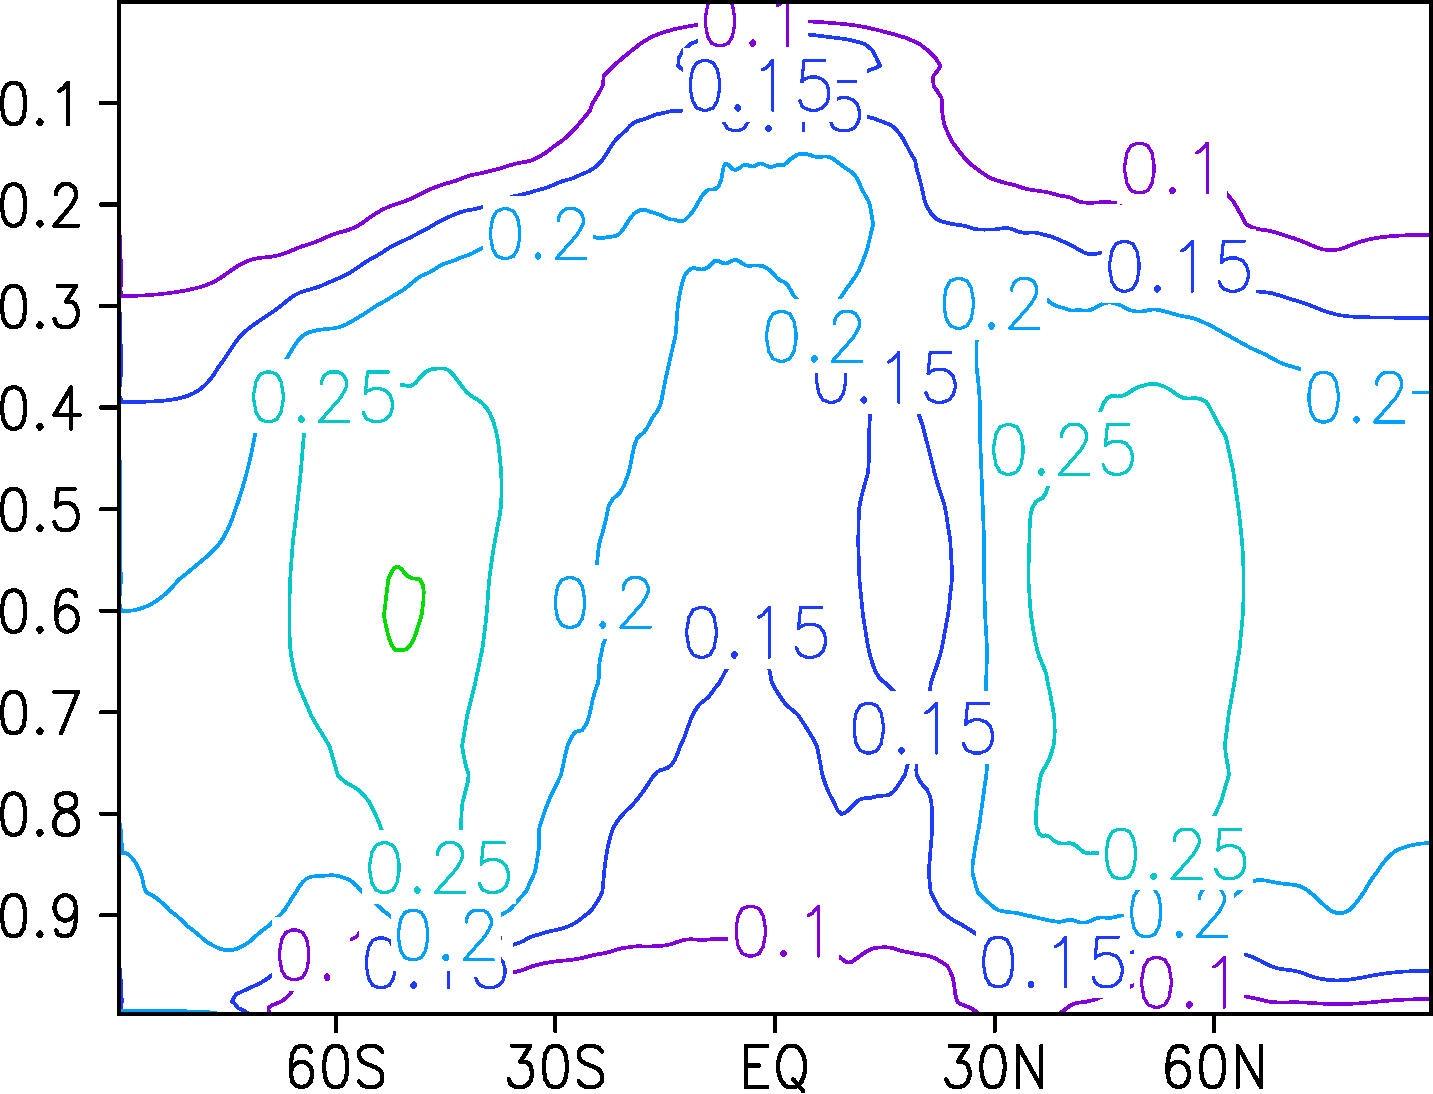
\includegraphics[width=0.3\textwidth,angle=0]{./figs/cap3/amplitudes_novas/amplitudes-B06Z_q-crop-rotated270.pdf}
        } \\
        
        \subfigure[$\mathbf{B}$ CPTEC (ALLZ), $q$]{
          \label{fig:bcptec_allz_q}
          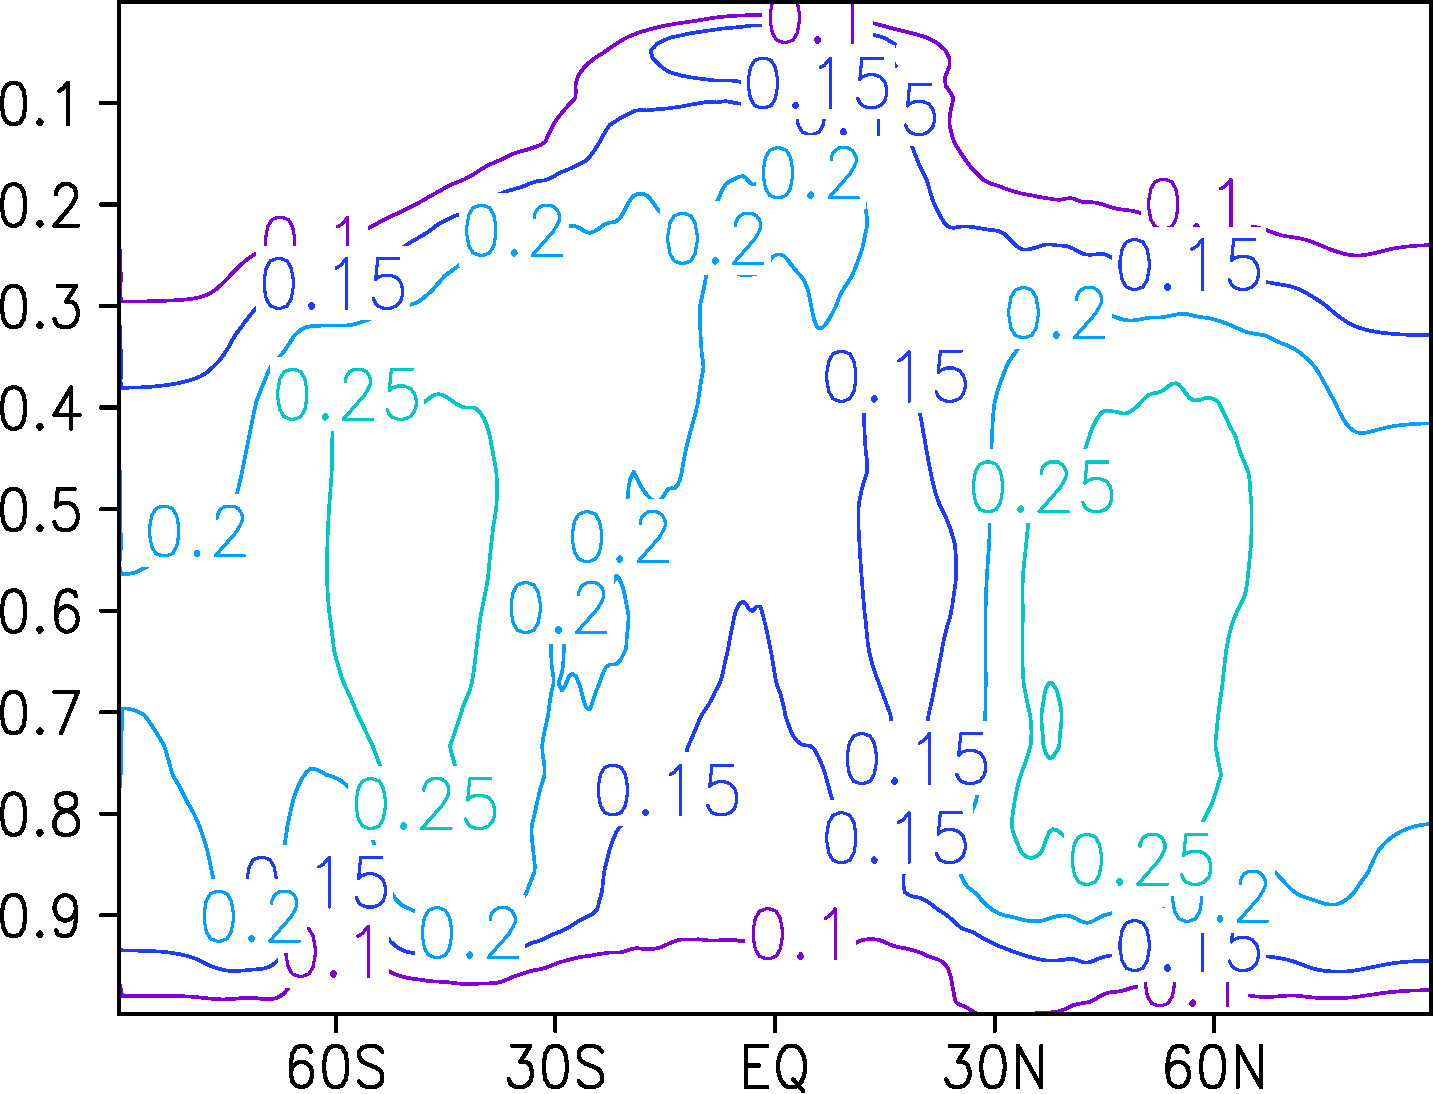
\includegraphics[width=0.3\textwidth,angle=0]{./figs/cap3/amplitudes_novas/amplitudes-BAllZ_q-crop-rotated270.pdf}
        }   
        \subfigure[$\mathbf{B}$ CPTEC (12Z), $q$]{
          \label{fig:bcptec_12z_q}
          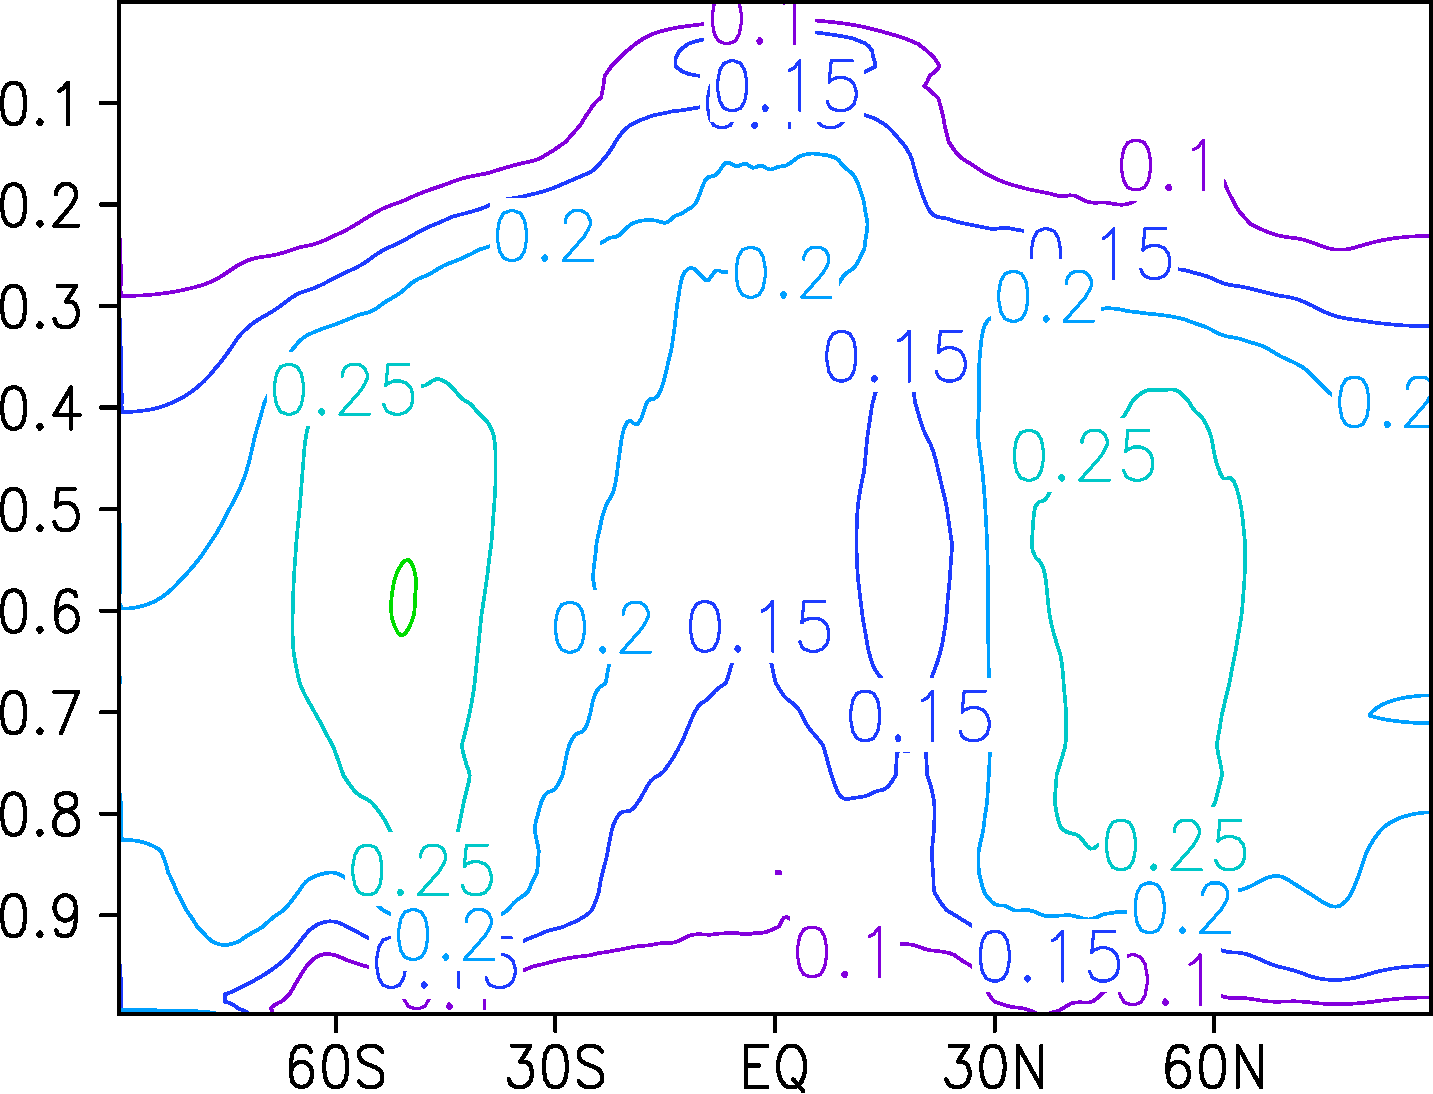
\includegraphics[width=0.3\textwidth,angle=0]{./figs/cap3/amplitudes_novas/amplitudes-B12Z_q-crop-rotated270.pdf}
        }    
        \subfigure[$\mathbf{B}$ CPTEC (18Z), $q$]{
          \label{fig:bcptec_18z_q}
          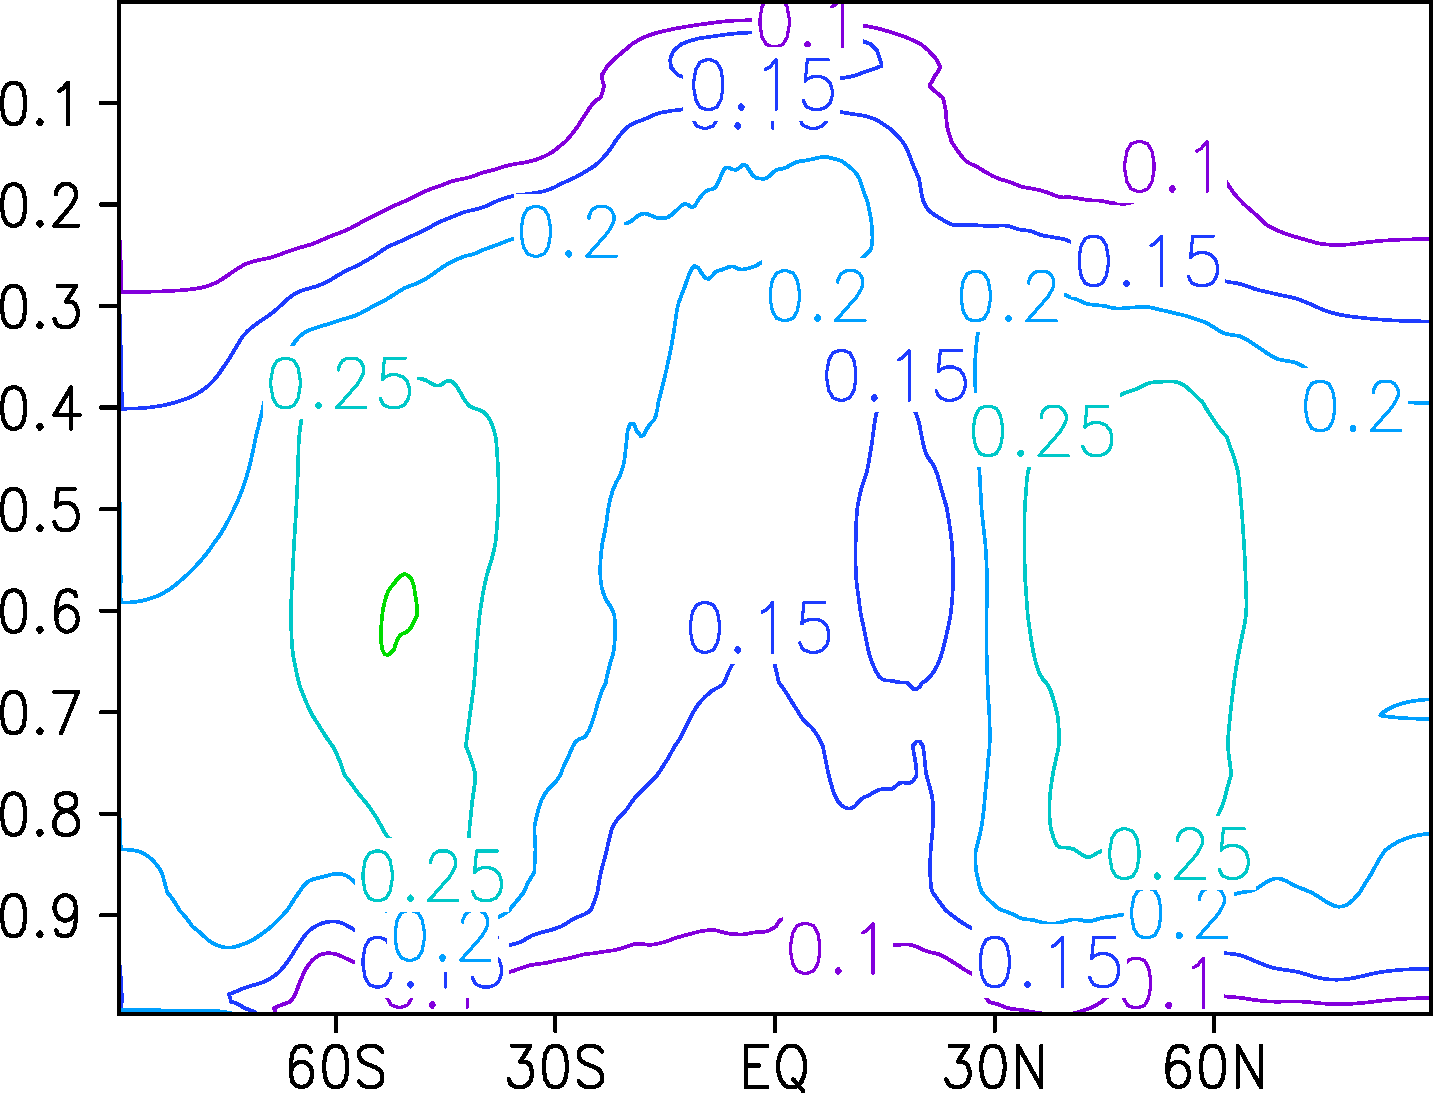
\includegraphics[width=0.3\textwidth,angle=0]{./figs/cap3/amplitudes_novas/amplitudes-B18Z_q-crop-rotated270.pdf}
        }   
  \end{center}
  \vspace{2mm}
  \legenda{}
  \label{fig:B_mcgav4_q}
  \FONTE{Produção do autor.}
\end{figure}

A Figura \ref{fig:B_mcgav4_ps} apresenta a distribuição latitudinal das médias zonais das amplitudes da pressão em superfície. As amplitudes da matriz B NCEP (Figura \ref{fig:bncep_allz_ps}) apresentam uma distribuição simétrica, com dois picos sobre as latitudes de 60S e 60N. Nas matrizes do CPTEC (Figuras \ref{fig:bcptec_00z_ps}, \ref{fig:bcptec_06z_ps}, \ref{fig:bcptec_allz_ps}, \ref{fig:bcptec_12z_ps} e \ref{fig:bcptec_18z_ps}), a distribuição das amplitudes é assimétrica, sendo que os picos das amplitudes são maiores sobre a latitude de 60N do que sobre a latitude de 60S. A mesma amplitude apresentada em \citeonline{wuetal/2002}, mostra que os picos da variância dos erros situam-se em torno destas latitudes, especialmente sobre o Hemisfério Norte, onde o pico local situa-se entre as latitudes de 30N e 60N.

\begin{figure}[H]
  \vspace{2mm}
    \caption{Idem Figura \ref{fig:B_mcgav4_psi}, para a pressão em superfície ($ps$, x $10^{2}$).}
    \begin{center}
        \subfigure[$\mathbf{B}$ NCEP (ALLZ), $ps$]{
          \label{fig:bncep_allz_ps}
          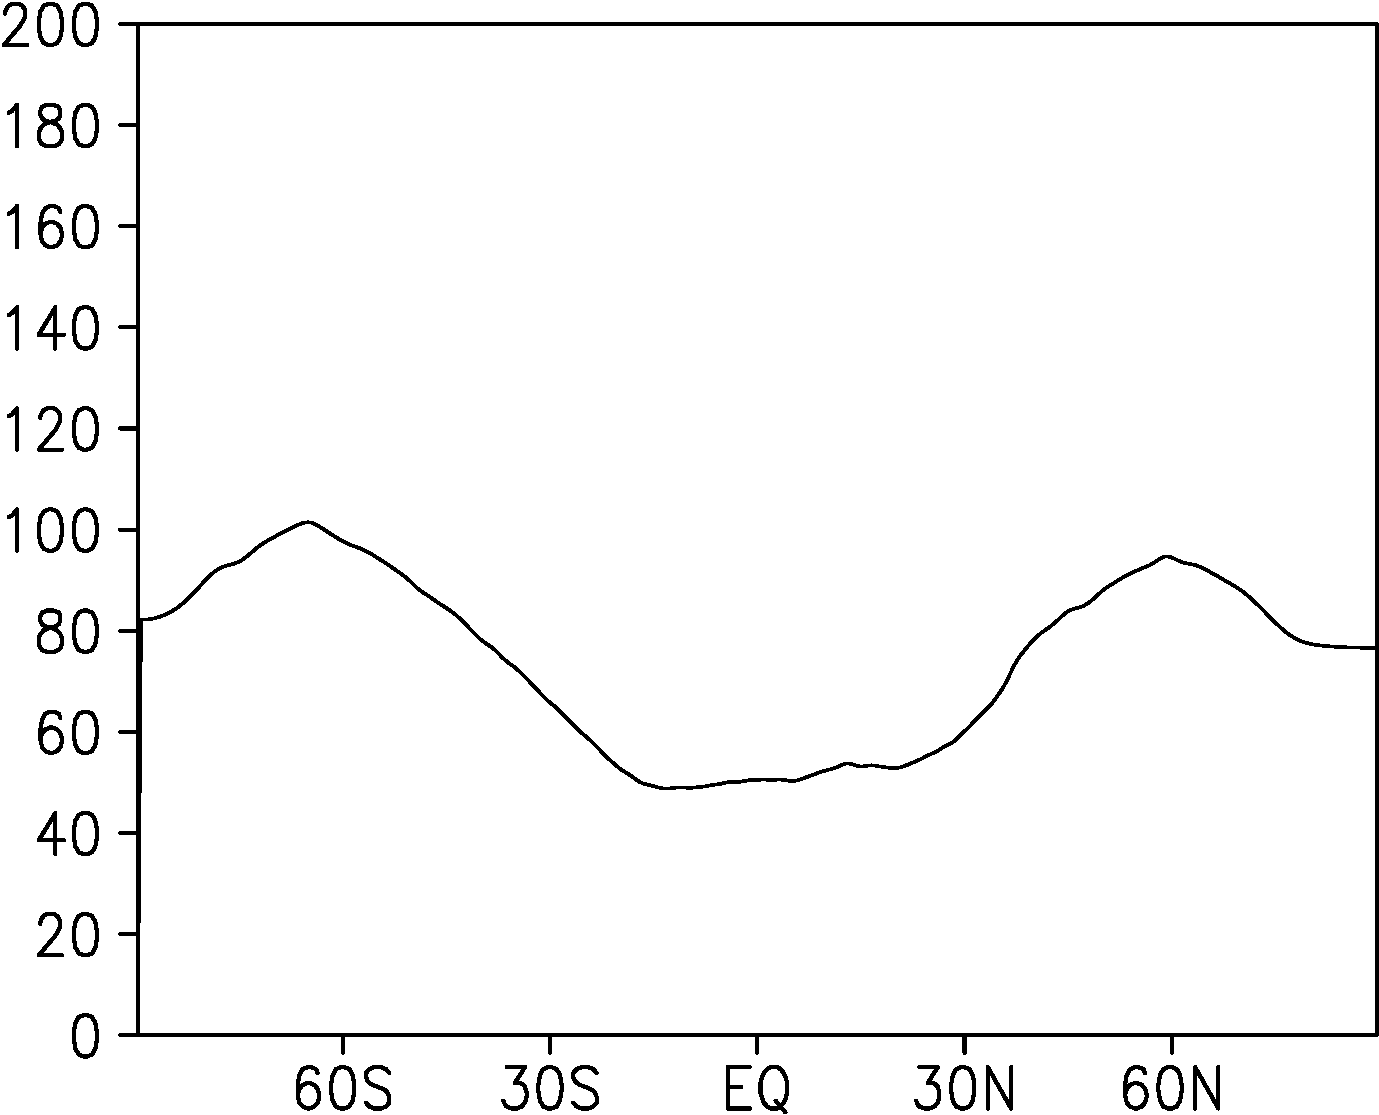
\includegraphics[width=0.3\textwidth,angle=0]{./figs/cap3/amplitudes_novas/amplitudes-NCEP_ps-crop-rotated270.pdf}
        }
        \subfigure[$\mathbf{B}$ CPTEC (00Z), $ps$]{
          \label{fig:bcptec_00z_ps}
          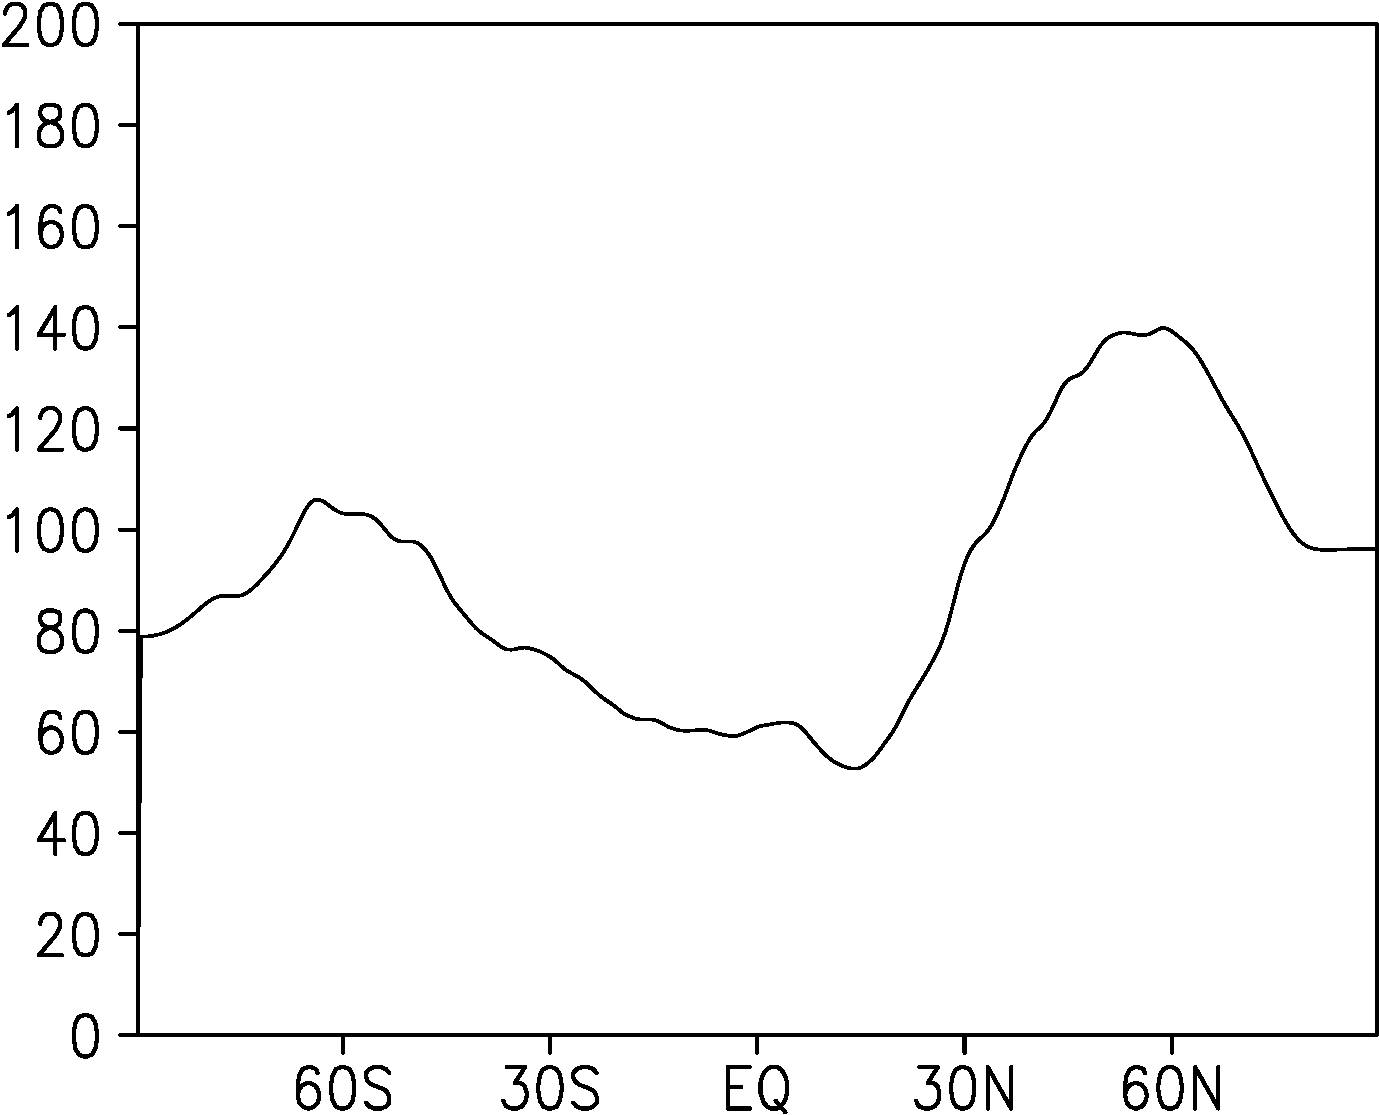
\includegraphics[width=0.3\textwidth,angle=0]{./figs/cap3/amplitudes_novas/amplitudes-B00Z_ps-crop-rotated270.pdf}
        } 
        \subfigure[$\mathbf{B}$ CPTEC (06Z), $ps$]{
          \label{fig:bcptec_06z_ps}
          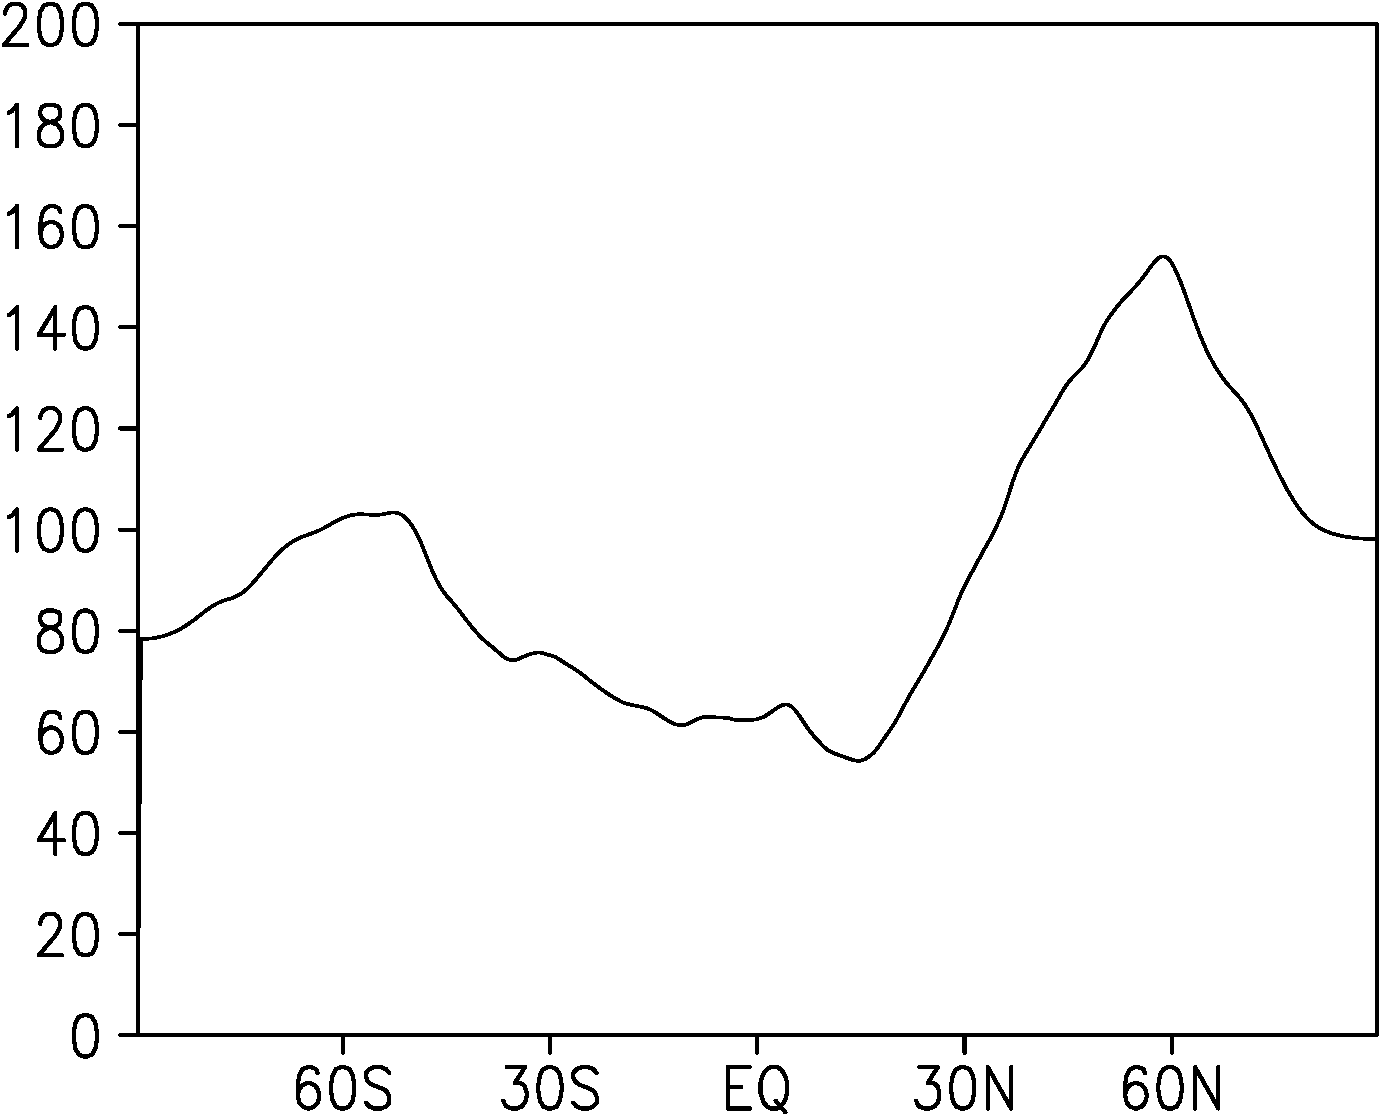
\includegraphics[width=0.3\textwidth,angle=0]{./figs/cap3/amplitudes_novas/amplitudes-B06Z_ps-crop-rotated270.pdf}
        } \\
        
        \subfigure[$\mathbf{B}$ CPTEC (ALLZ), $ps$]{
          \label{fig:bcptec_allz_ps}
          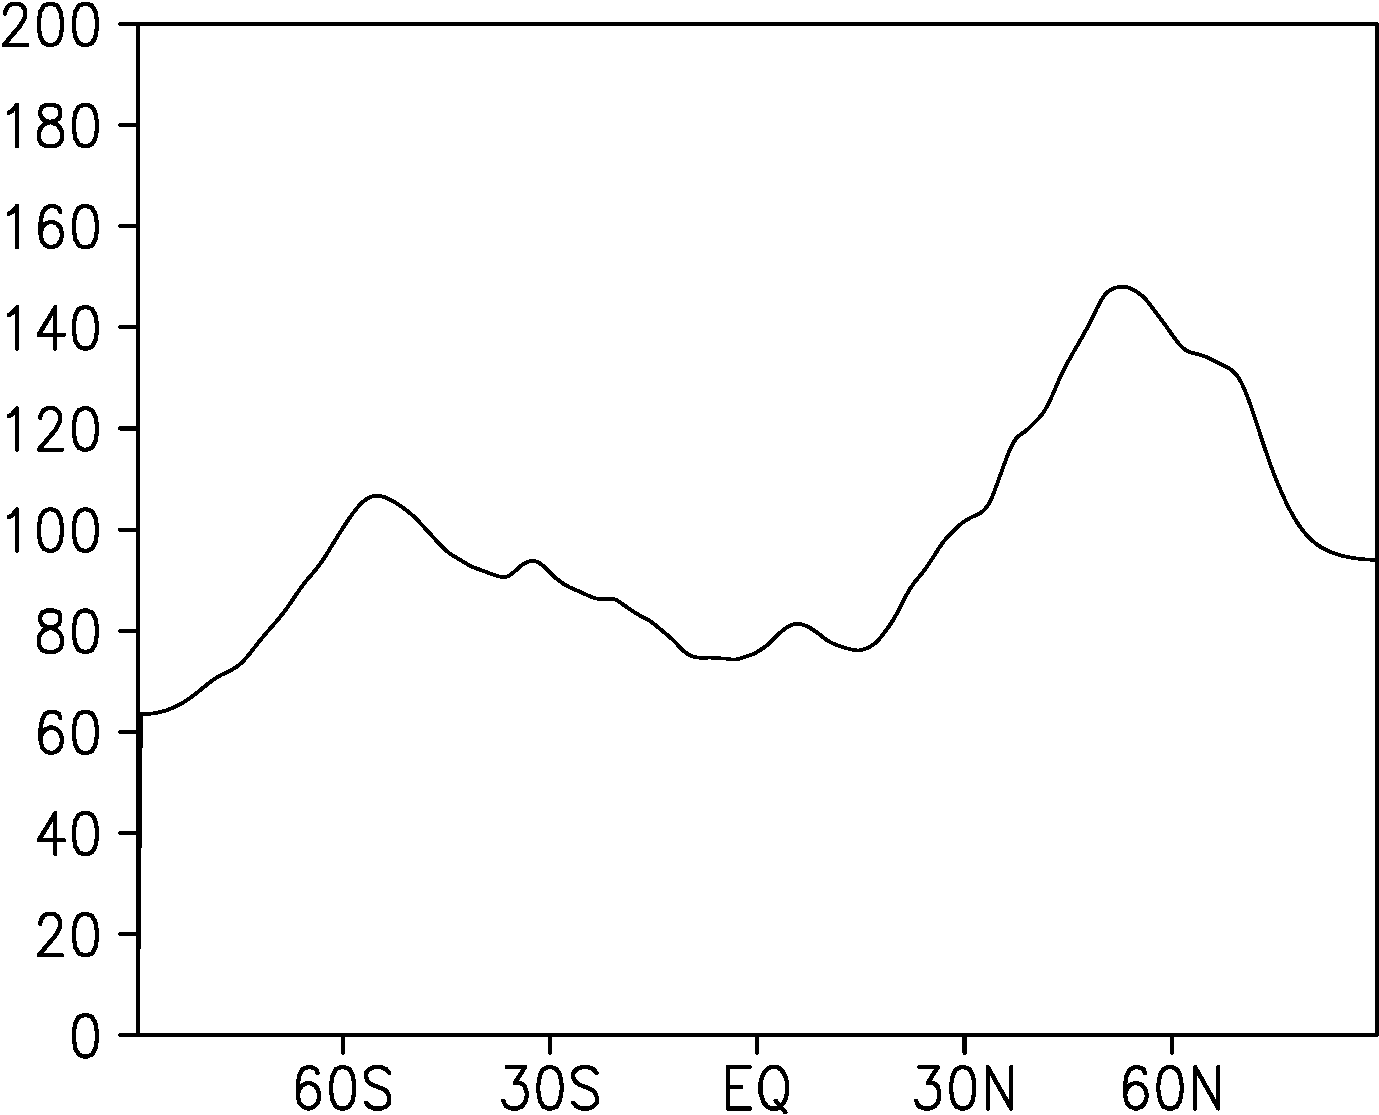
\includegraphics[width=0.3\textwidth,angle=0]{./figs/cap3/amplitudes_novas/amplitudes-BAllZ_ps-crop-rotated270.pdf}
        }   
        \subfigure[$\mathbf{B}$ CPTEC (12Z), $ps$]{
          \label{fig:bcptec_12z_ps}
          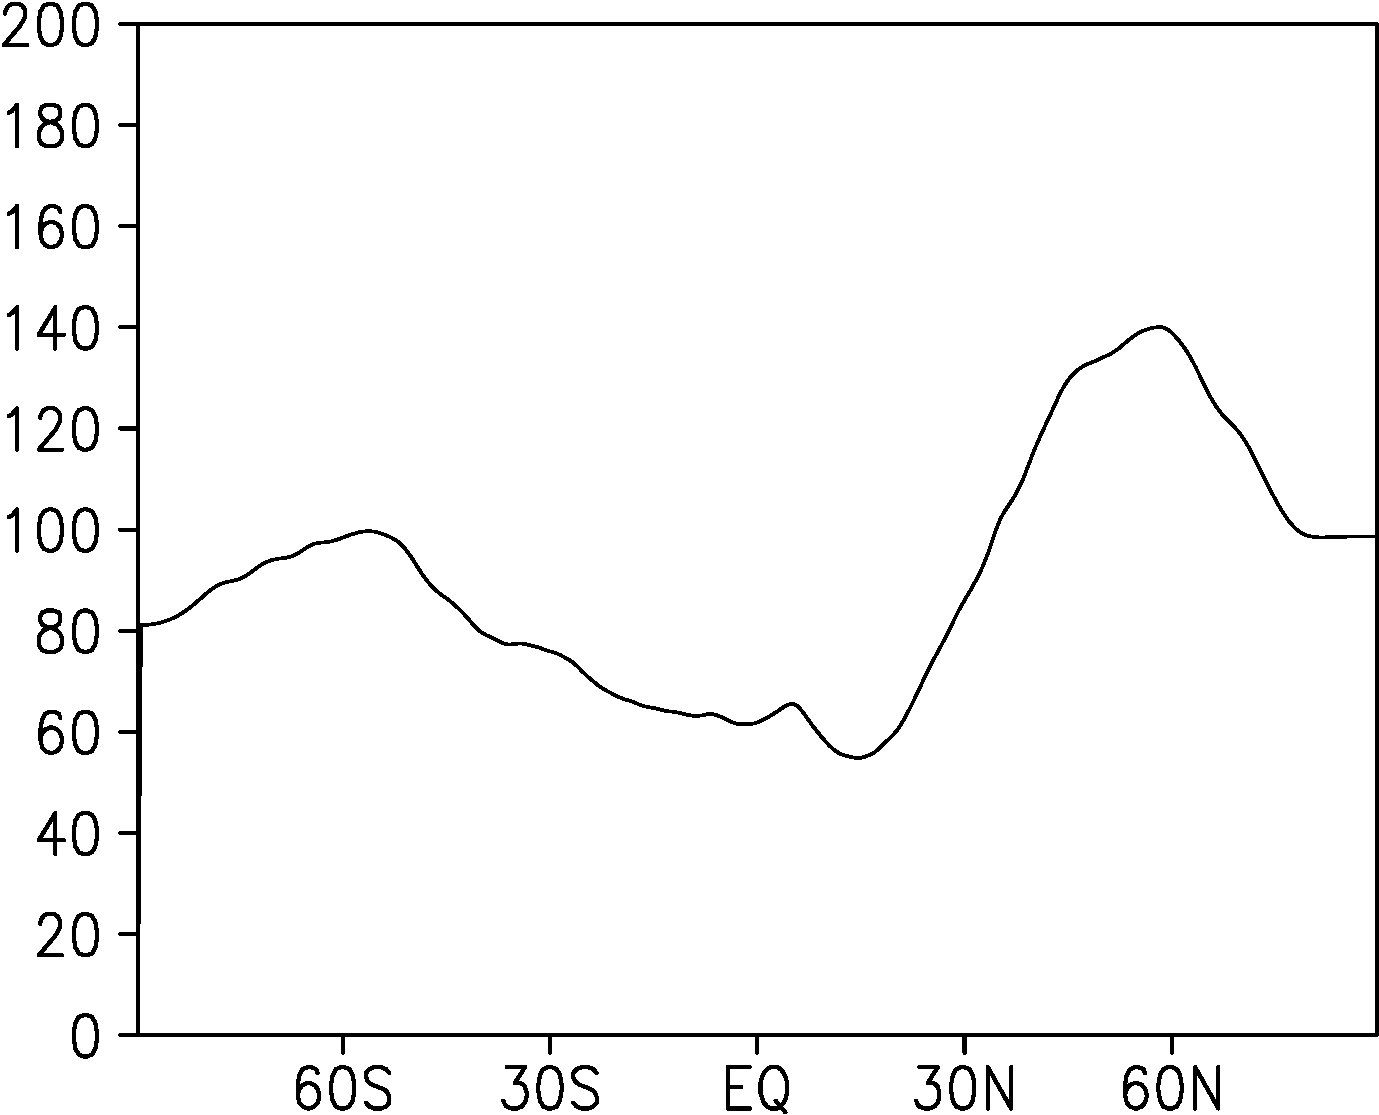
\includegraphics[width=0.3\textwidth,angle=0]{./figs/cap3/amplitudes_novas/amplitudes-B12Z_ps-crop-rotated270.pdf}
        }    
        \subfigure[$\mathbf{B}$ CPTEC (18Z), $ps$]{
          \label{fig:bcptec_18z_ps}
          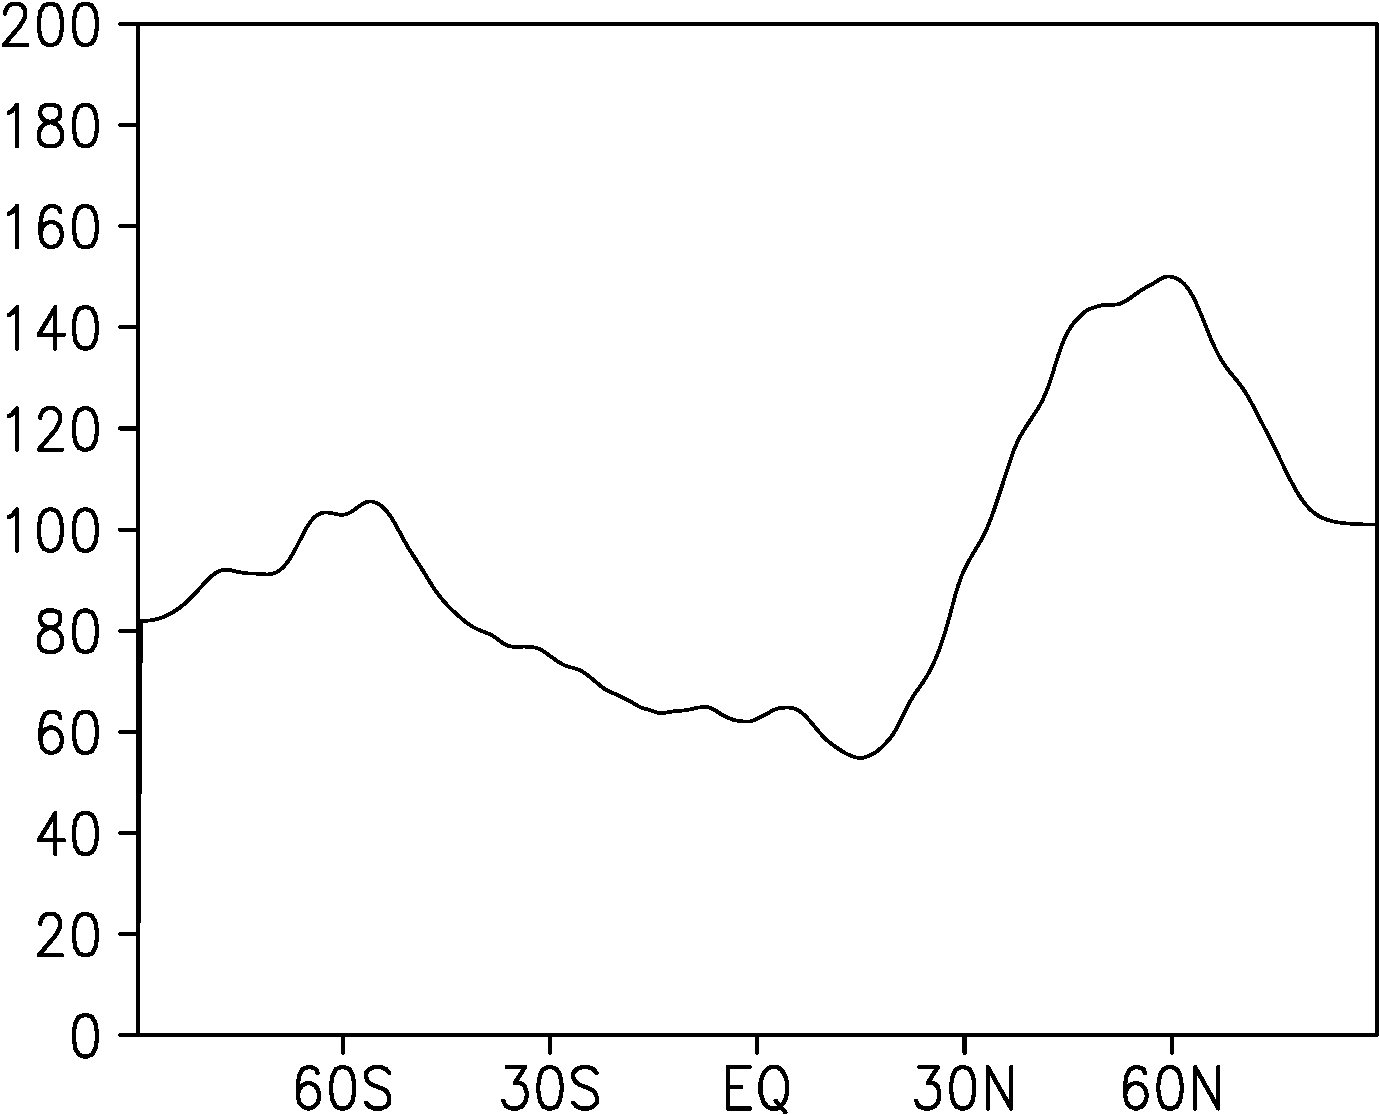
\includegraphics[width=0.3\textwidth,angle=0]{./figs/cap3/amplitudes_novas/amplitudes-B18Z_ps-crop-rotated270.pdf}
        }   
  \end{center} 
  \vspace{2mm}
  \legenda{}
  \label{fig:B_mcgav4_ps}
  \FONTE{Produção do autor.}
\end{figure}

As Figuras \ref{fig:bncep_allz_oz_zlog}, \ref{fig:bcptec_00z_oz} e a Figura \ref{fig:bcptec_allz_cw} mostram as amplitudes calculadas para as variáveis ozônio e razão de mistura de condensação em nuvem, respectivamente. O sistema G3DVAR (versão v1.1.3) não assimila observações e ozônio, e além disso, o ozônio utilizado pelo modelo de MCGAv4 utiliza uma climatologia do ozônio. As amplitudes calculadas para esta quantidade são bastante diferentes daquelas apresentadas pela matriz NCEP BAllZ (Figuras \ref{fig:bncep_allz_oz_zlog}, \ref{fig:bcptec_00z_oz}), e mostram valores muito mais altos do que qualquer matriz calculada utilizando-se os pares de previsões do CPTEC. Além disso, o MCGAv4 não representa a razão de mistura de condensação, como pode ser visto na Figura \ref{fig:bcptec_allz_cw}. Para melhorar a visualização da distribuição das amplitudes do ozônio, na Figura \ref{fig:bncep_allz_oz_zlog} estas amplitudes estão destacadas em escala logarítmica. 

\begin{figure}[H]
  \vspace{2mm}
    \caption{Idem Figura \ref{fig:B_mcgav4_psi}, para o ozônio ($oz$ x $10^{7}$) e o conteúdo de água ($cw$  x $10^{4}$).}
    \begin{center}
        \subfigure[$\mathbf{B}$ NCEP (ALLZ), $log(oz)$]{
          \label{fig:bncep_allz_oz_zlog}
          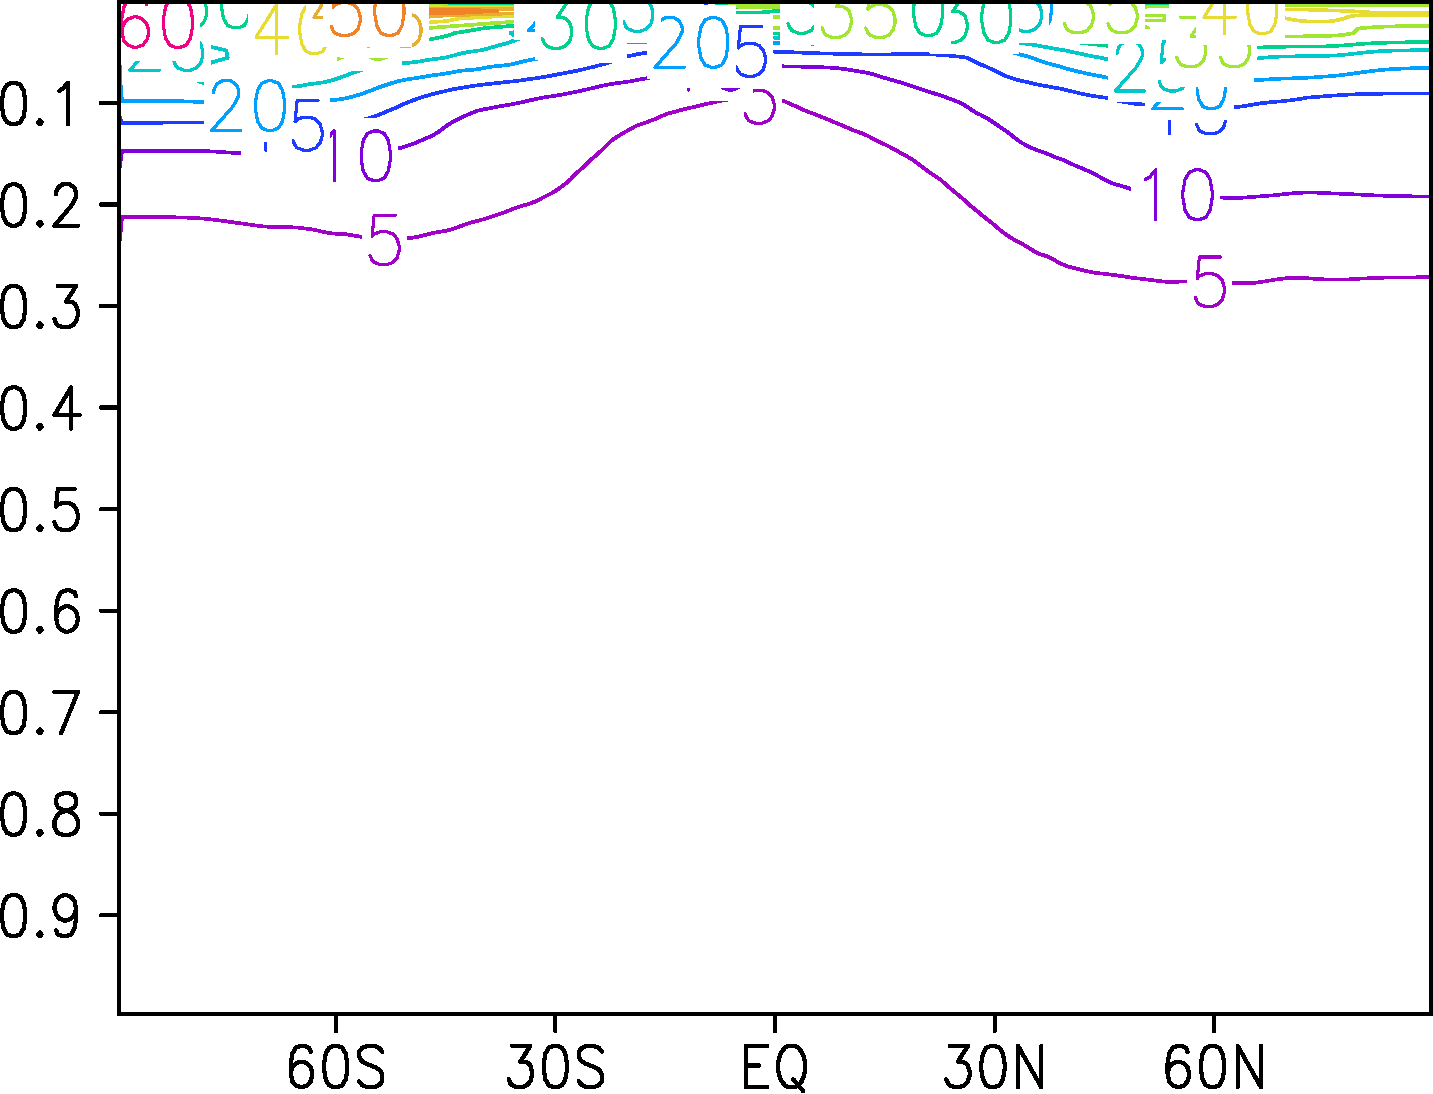
\includegraphics[width=0.3\textwidth,angle=0]{./figs/cap3/amplitudes_novas/amplitudes-NCEP_oz-orig-crop-rotated270.pdf}
        }
        \subfigure[$\mathbf{B}$ NCEP (ALLZ), $oz$]{
          \label{fig:bcptec_00z_oz}
          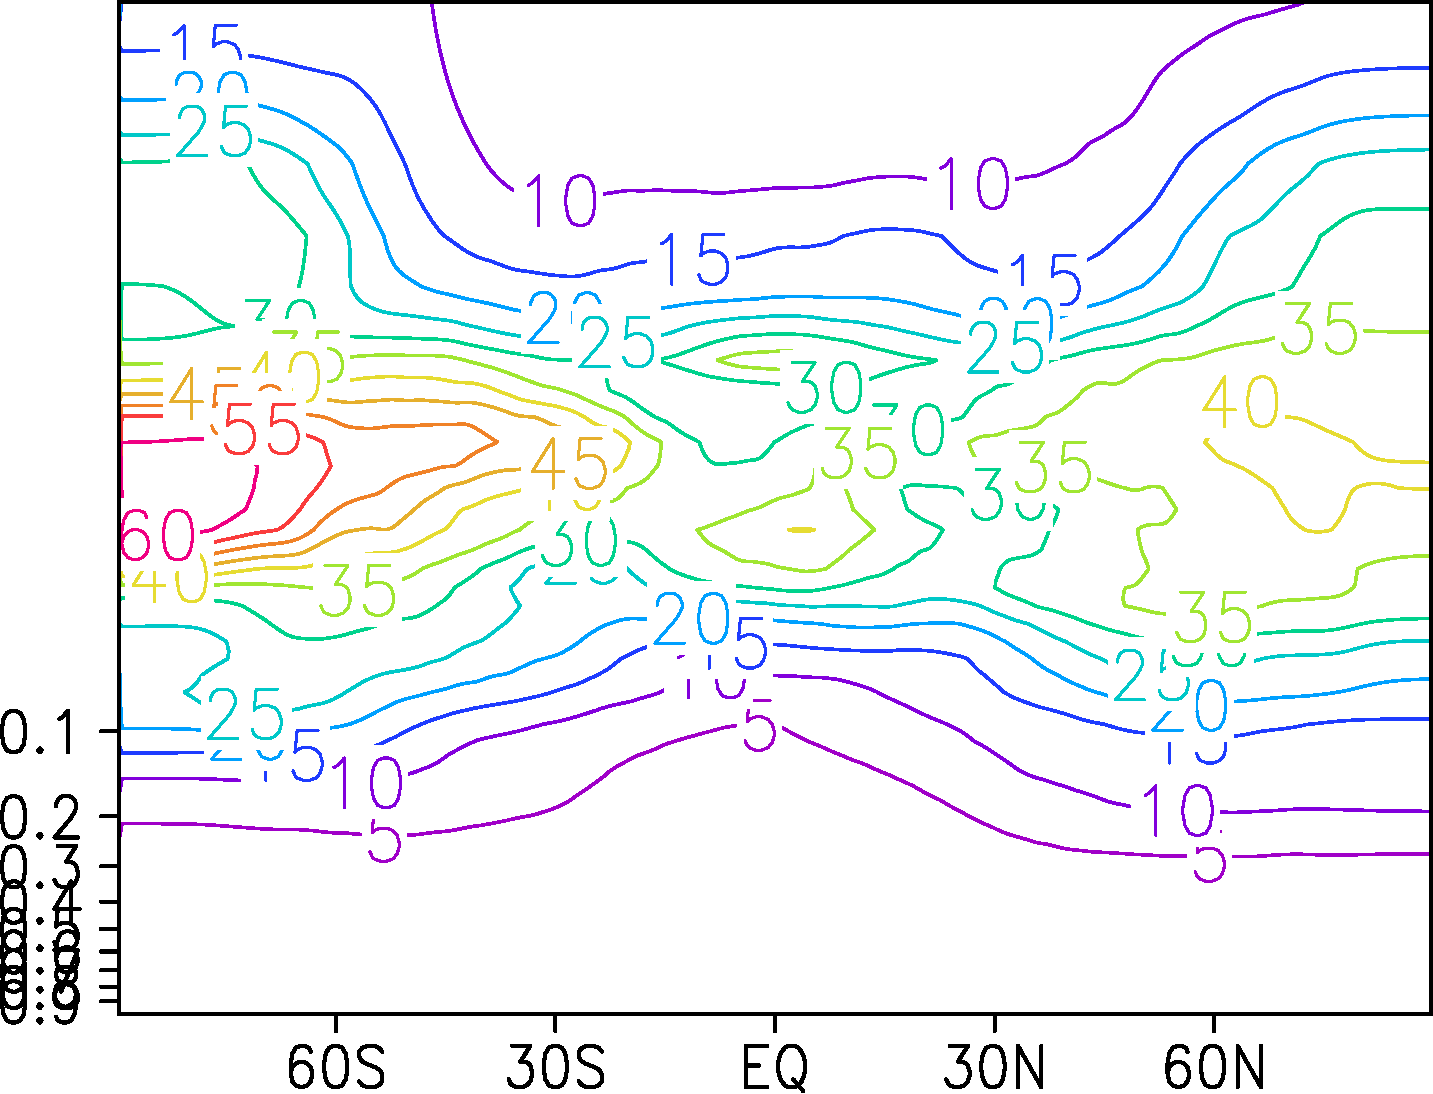
\includegraphics[width=0.3\textwidth,angle=0]{./figs/cap3/amplitudes_novas/amplitudes-NCEP_oz_zlog-orig-crop-rotated270.pdf}
        }         
        \subfigure[$\mathbf{B}$ NCEP (ALLZ), $cw$]{
          \label{fig:bcptec_allz_cw}
          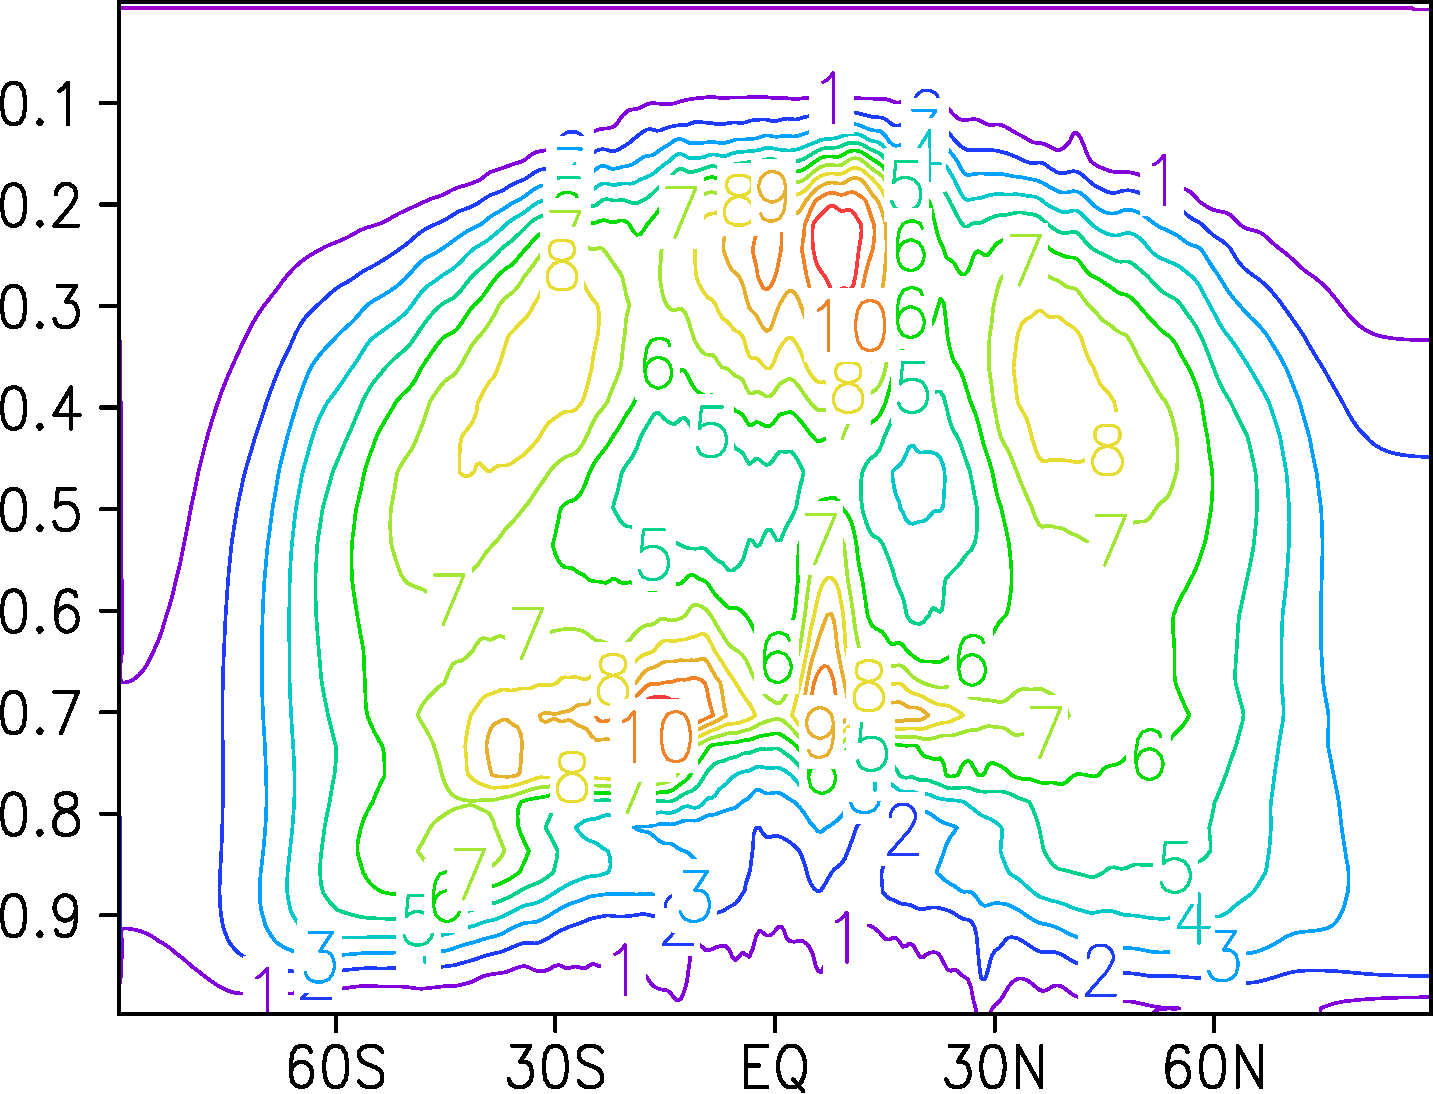
\includegraphics[width=0.3\textwidth,angle=0]{./figs/cap3/amplitudes_novas/amplitudes-NCEP_cw-orig-crop-rotated270.pdf}
        }   
    \end{center}
  \vspace{2mm}
  \legenda{}
  \label{fig:B_mcgav4_oz_cw}
  \FONTE{Produção do autor.}
\end{figure}

Nas Tabelas \ref{tab:amplimaxminB}, \ref{tab:comphorizmaxminB} e \ref{tab:compvertmaxminB} são apresentados os valores máximos e mínimos das quantidades apresentadas nas Figuras \ref{fig:B_mcgav4_psi}, \ref{fig:B_mcgav4_chi}, \ref{fig:B_mcgav4_T}, \ref{fig:B_mcgav4_q}, \ref{fig:B_mcgav4_ps} e \ref{fig:B_mcgav4_oz_cw} em adição as amplitudes e comprimentos de escalas da temperatura da superfície do mar.

\begin{table}[H]
\caption{Valores máximos e mínimos das amplitudes das versões das matrizes de covariâncias do CPTEC na resolução TQ0299L064 a partir dos pares de previsões de 48 e 24 horas do modelo MCGAv4.}
\begin{center}
\begin{adjustbox}{max width=\textwidth}
\begin{tabular}{ccccccccccccc}
\toprule
\toprule
\multicolumn{1}{c}{} & \multicolumn{2}{c}{\textbf{Bncep}} & \multicolumn{2}{c}{\textbf{Bcptec}} & \multicolumn{2}{c}{\textbf{B00Zcptec}} &\multicolumn{2}{c}{\textbf{B06Zcptec}} & \multicolumn{2}{c}{\textbf{B12Zcptec}} & \multicolumn{2}{c}{\textbf{B18Zcptec}} \\
\cmidrule(lr){2-3} \cmidrule(lr){4-5} \cmidrule(lr){6-7} \cmidrule(lr){8-9} \cmidrule(lr){10-11} \cmidrule(lr){12-13} 
\multicolumn{1}{c}{} & \multicolumn{1}{c}{\textbf{Máx}} & \multicolumn{1}{c}{\textbf{Mín}} & \multicolumn{1}{c}{\textbf{Máx}} & \multicolumn{1}{c}{\textbf{Mín}} & \multicolumn{1}{c}{\textbf{Máx}} & \multicolumn{1}{c}{\textbf{Mín}} & \multicolumn{1}{c}{\textbf{Máx}} & \multicolumn{1}{c}{\textbf{Mín}} & \multicolumn{1}{c}{\textbf{Máx}} & \multicolumn{1}{c}{\textbf{Mín}} & \multicolumn{1}{c}{\textbf{Máx}} & \multicolumn{1}{c}{\textbf{Mín}} \\
\midrule   
\multicolumn{1}{c}{$\psi$} & \multicolumn{1}{c}{7,99x$10^{6}$} & \multicolumn{1}{c}{4,3x$10^{5}$} & \multicolumn{1}{c}{2,8x$10^{7}$} & \multicolumn{1}{c}{4,6x$10^{5}$} & \multicolumn{1}{c}{1,7x$10^{7}$} & \multicolumn{1}{c}{4,9x$10^{5}$} & \multicolumn{1}{c}{1,9x$10^{7}$} & \multicolumn{1}{c}{4,9x$10^{5}$} & \multicolumn{1}{c}{1,7x$10^{7}$} & \multicolumn{1}{c}{4,9x$10^{5}$} & \multicolumn{1}{c}{1,7x$10^{7}$} & \multicolumn{1}{c}{4,8x$10^{5}$}  \\ 
\multicolumn{1}{c}{$\chi$} & \multicolumn{1}{c}{3,77x$10^{6}$} & \multicolumn{1}{c}{0} & \multicolumn{1}{c}{1,07x$10^{7}$} & \multicolumn{1}{c}{0} & \multicolumn{1}{c}{4,52x$10^{6}$} & \multicolumn{1}{c}{0} & \multicolumn{1}{c}{3,74x$10^{6}$} & \multicolumn{1}{c}{0} & \multicolumn{1}{c}{4,19x$10^{6}$} & \multicolumn{1}{c}{0} & \multicolumn{1}{c}{4,94x$10^{6}$} & \multicolumn{1}{c}{0} \\ 
\multicolumn{1}{c}{$T$}    & \multicolumn{1}{c}{2,23} & \multicolumn{1}{c}{0} & \multicolumn{1}{c}{4,04} & \multicolumn{1}{c}{0} & \multicolumn{1}{c}{3,01} & \multicolumn{1}{c}{0} & \multicolumn{1}{c}{3,11} & \multicolumn{1}{c}{0} & \multicolumn{1}{c}{3,13} & \multicolumn{1}{c}{0} & \multicolumn{1}{c}{3,03} & \multicolumn{1}{c}{0} \\ 
\multicolumn{1}{c}{$q$}    & \multicolumn{1}{c}{0,41} & \multicolumn{1}{c}{-4,06x$10^{-7}$} & \multicolumn{1}{c}{0,29} & \multicolumn{1}{c}{-2,15x$10^{-7}$} & \multicolumn{1}{c}{0,3} & \multicolumn{1}{c}{-2,12x$10^{-7}$} & \multicolumn{1}{c}{0,3} & \multicolumn{1}{c}{-2,27x$10^{-7}$} & \multicolumn{1}{c}{0,3} & \multicolumn{1}{c}{-2,59x$10^{-7}$} & \multicolumn{1}{c}{0,3} & \multicolumn{1}{c}{-2,53x$10^{-7}$} \\ 
\multicolumn{1}{c}{$oz$}  & \multicolumn{1}{c}{6,4x$10^{-7}$} & \multicolumn{1}{c}{-4,38x$10^{-7}$} & \multicolumn{1}{c}{4,4x$10^{-7}$} & \multicolumn{1}{c}{-2,2x$10^{-7}$} & \multicolumn{1}{c}{6,4x$10^{-7}$} & \multicolumn{1}{c}{-2,30x$10^{-7}$} & \multicolumn{1}{c}{6,4x$10^{-7}$} & \multicolumn{1}{c}{-2,33x$10^{-7}$} & \multicolumn{1}{c}{6,4x$10^{-7}$} & \multicolumn{1}{c}{-2,59x$10^{-7}$} & \multicolumn{1}{c}{6,4x$10^{-7}$} & \multicolumn{1}{c}{-2,63x$10^{-7}$} \\ 
\multicolumn{1}{c}{$cw$}  & \multicolumn{1}{c}{1,24x$10^{-4}$} & \multicolumn{1}{c}{-4,4x$10^{-7}$} & \multicolumn{1}{c}{1,24x$10^{-4}$} & \multicolumn{1}{c}{-2,4x$10^{-7}$} & \multicolumn{1}{c}{1,24x$10^{-4}$} & \multicolumn{1}{c}{-2,3x$10^{-7}$} & \multicolumn{1}{c}{1,24x$10^{-4}$} & \multicolumn{1}{c}{-2,33x$10^{-7}$} & \multicolumn{1}{c}{1,24x$10^{-4}$} & \multicolumn{1}{c}{-2,59x$10^{-7}$} & \multicolumn{1}{c}{1,24x$10^{-4}$} & \multicolumn{1}{c}{-2,64x$10^{-7}$} \\ 
\multicolumn{1}{c}{$ps$}   & \multicolumn{1}{c}{1,01x$10^{-1}$} & \multicolumn{1}{c}{4,88x$10^{-2}$} & \multicolumn{1}{c}{1,48x$10^{-1}$} & \multicolumn{1}{c}{6,35x$10^{-2}$} & \multicolumn{1}{c}{1,4x$10^{-1}$} & \multicolumn{1}{c}{5,27x$10^{-2}$} & \multicolumn{1}{c}{1,54x$10^{-1}$} & \multicolumn{1}{c}{5,43x$10^{-2}$} & \multicolumn{1}{c}{1,4x$10^{-1}$} & \multicolumn{1}{c}{5,48x$10^{-2}$} & \multicolumn{1}{c}{1,5x$10^{-1}$} & \multicolumn{1}{c}{5,48x$10^{-2}$} \\ 
\multicolumn{1}{c}{$sst$} & \multicolumn{1}{c}{4,32x$10^{-1}$} & \multicolumn{1}{c}{2x$10^{-1}$} & \multicolumn{1}{c}{4,32x$10^{-1}$} & \multicolumn{1}{c}{2x$10^{-1}$} & \multicolumn{1}{c}{4,32x$10^{-1}$} & \multicolumn{1}{c}{2x$10^{-1}$} & \multicolumn{1}{c}{4,32x$10^{-1}$} & \multicolumn{1}{c}{2x$10^{-1}$} & \multicolumn{1}{c}{4,32x$10^{-1}$} & \multicolumn{1}{c}{2x$10^{-1}$} & \multicolumn{1}{c}{4,32x$10^{-1}$} & \multicolumn{1}{c}{2x$10^{-1}$} \\ 
\bottomrule
\end{tabular}
\end{adjustbox}
\end{center}
\label{tab:amplimaxminB}
\end{table}

\begin{table}[H]
\caption{Idem Tabela \ref{tab:amplimaxminB}, para os comprimentos de escala horizontais.}
\begin{center}
\begin{adjustbox}{max width=\textwidth}
\begin{tabular}{ccccccccccccc}
\toprule
\toprule
\multicolumn{1}{c}{} & \multicolumn{2}{c}{\textbf{Bncep}} & \multicolumn{2}{c}{\textbf{Bcptec}} & \multicolumn{2}{c}{\textbf{B00Zcptec}} &\multicolumn{2}{c}{\textbf{B06Zcptec}} & \multicolumn{2}{c}{\textbf{B12Zcptec}} & \multicolumn{2}{c}{\textbf{B18Zcptec}} \\
\cmidrule(lr){2-3} \cmidrule(lr){4-5} \cmidrule(lr){6-7} \cmidrule(lr){8-9} \cmidrule(lr){10-11} \cmidrule(lr){12-13}
\multicolumn{1}{c}{} & \multicolumn{1}{c}{\textbf{Máx}} & \multicolumn{1}{c}{\textbf{Mín}} & \multicolumn{1}{c}{\textbf{Máx}} & \multicolumn{1}{c}{\textbf{Mín}} & \multicolumn{1}{c}{\textbf{Máx}} & \multicolumn{1}{c}{\textbf{Mín}} & \multicolumn{1}{c}{\textbf{Máx}} & \multicolumn{1}{c}{\textbf{Mín}} & \multicolumn{1}{c}{\textbf{Máx}} & \multicolumn{1}{c}{\textbf{Mín}} & \multicolumn{1}{c}{\textbf{Máx}} & \multicolumn{1}{c}{\textbf{Mín}} \\
\midrule
\multicolumn{1}{c}{$\psi$} & \multicolumn{1}{c}{1,3x$10^{6}$} & \multicolumn{1}{c}{2,2x$10^{5}$} & \multicolumn{1}{c}{1,75x$10^{6}$} & \multicolumn{1}{c}{4,55x$10^{5}$} & \multicolumn{1}{c}{1,32x$10^{6}$} & \multicolumn{1}{c}{4,73x$10^{5}$} & \multicolumn{1}{c}{1,4x$10^{6}$} & \multicolumn{1}{c}{4,7x$10^{5}$} & \multicolumn{1}{c}{1,31x$10^{6}$} & \multicolumn{1}{c}{4,7x$10^{5}$} & \multicolumn{1}{c}{1,27x$10^{6}$} & \multicolumn{1}{c}{4,73x$10^{5}$} \\ 
\multicolumn{1}{c}{$\chi$} & \multicolumn{1}{c}{1,1x$10^{6}$} & \multicolumn{1}{c}{0} & \multicolumn{1}{c}{1,82x$10^{6}$} & \multicolumn{1}{c}{0} & \multicolumn{1}{c}{1,37x$10^{6}$} & \multicolumn{1}{c}{0} & \multicolumn{1}{c}{1,45x$10^{6}$} & \multicolumn{1}{c}{0} & \multicolumn{1}{c}{1,5x$10^{6}$} & \multicolumn{1}{c}{0} & \multicolumn{1}{c}{1,42x$10^{6}$} & \multicolumn{1}{c}{0} \\ 
\multicolumn{1}{c}{$T$}    & \multicolumn{1}{c}{3,1x$10^{5}$} & \multicolumn{1}{c}{0} & \multicolumn{1}{c}{5,9x$10^{5}$} & \multicolumn{1}{c}{0} & \multicolumn{1}{c}{5,94x$10^{5}$} & \multicolumn{1}{c}{0} & \multicolumn{1}{c}{5,9x$10^{5}$} & \multicolumn{1}{c}{0} & \multicolumn{1}{c}{6,42x$10^{5}$} & \multicolumn{1}{c}{0} & \multicolumn{1}{c}{6,37x$10^{5}$} & \multicolumn{1}{c}{0} \\ 
\multicolumn{1}{c}{$q$}    & \multicolumn{1}{c}{7,9x$10^{6}$} & \multicolumn{1}{c}{0} & \multicolumn{1}{c}{2,22x$10^{7}$} & \multicolumn{1}{c}{0} & \multicolumn{1}{c}{1,31x$10^{7}$} & \multicolumn{1}{c}{0} & \multicolumn{1}{c}{1,48x$10^{7}$} & \multicolumn{1}{c}{0} & \multicolumn{1}{c}{1,33x$10^{7}$} & \multicolumn{1}{c}{0} & \multicolumn{1}{c}{1,36x$10^{7}$} & \multicolumn{1}{c}{0} \\ 
\multicolumn{1}{c}{$oz$}   & \multicolumn{1}{c}{7,99x$10^{6}$} & \multicolumn{1}{c}{0} & \multicolumn{1}{c}{2,84x$10^{7}$} & \multicolumn{1}{c}{0} & \multicolumn{1}{c}{1,73x$10^{7}$} & \multicolumn{1}{c}{0} & \multicolumn{1}{c}{1,96x$10^{7}$} & \multicolumn{1}{c}{0} & \multicolumn{1}{c}{1,75x$10^{7}$} & \multicolumn{1}{c}{0} & \multicolumn{1}{c}{1,78x$10^{7}$} & \multicolumn{1}{c}{0} \\ 
\multicolumn{1}{c}{$cw$}   & \multicolumn{1}{c}{7,99x$10^{6}$} & \multicolumn{1}{c}{0} & \multicolumn{1}{c}{2,84x$10^{7}$} & \multicolumn{1}{c}{0} & \multicolumn{1}{c}{1,73x$10^{7}$} & \multicolumn{1}{c}{0} & \multicolumn{1}{c}{1,96x$10^{7}$} & \multicolumn{1}{c}{0} & \multicolumn{1}{c}{1,75x$10^{7}$} & \multicolumn{1}{c}{0} & \multicolumn{1}{c}{1,78x$10^{7}$} & \multicolumn{1}{c}{0} \\ 
\multicolumn{1}{c}{$ps$}   & \multicolumn{1}{c}{1,89x$10^{5}$} & \multicolumn{1}{c}{1,19x$10^{5}$} & \multicolumn{1}{c}{4,18x$10^{5}$} & \multicolumn{1}{c}{1,83x$10^{5}$} & \multicolumn{1}{c}{3,9x$10^{5}$} & \multicolumn{1}{c}{1,83x$10^{5}$} & \multicolumn{1}{c}{3,9x$10^{5}$} & \multicolumn{1}{c}{1,8x$10^{5}$} & \multicolumn{1}{c}{3,8x$10^{5}$} & \multicolumn{1}{c}{1,8x$10^{5}$} & \multicolumn{1}{c}{3,9x$10^{5}$} & \multicolumn{1}{c}{1,84x$10^{5}$} \\ 
\multicolumn{1}{c}{$sst$}  & \multicolumn{1}{c}{8x$10^{2}$} & \multicolumn{1}{c}{5,07x$10^{2}$} & \multicolumn{1}{c}{8x$10^{2}$} & \multicolumn{1}{c}{5,07x$10^{2}$} & \multicolumn{1}{c}{8x$10^{2}$} & \multicolumn{1}{c}{5,07x$10^{2}$} & \multicolumn{1}{c}{8x$10^{2}$} & \multicolumn{1}{c}{5,07x$10^{2}$} & \multicolumn{1}{c}{8x$10^{2}$} & \multicolumn{1}{c}{5,07x$10^{2}$} & \multicolumn{1}{c}{8x$10^{2}$} & \multicolumn{1}{c}{5,07x$10^{2}$} \\ 
\bottomrule
\end{tabular}
\end{adjustbox}
\end{center}
\label{tab:comphorizmaxminB}
\end{table}

\begin{table}[H]
\caption{Idem Tabela \ref{tab:amplimaxminB}, para os comprimentos de escala verticais.}
\begin{center}
\begin{adjustbox}{max width=\textwidth}
\begin{tabular}{ccccccccccccc}
\toprule
\toprule
\multicolumn{1}{c}{} & \multicolumn{2}{c}{\textbf{Bncep}} & \multicolumn{2}{c}{\textbf{Bcptec}} & \multicolumn{2}{c}{\textbf{B00Zcptec}} &\multicolumn{2}{c}{\textbf{B06Zcptec}} & \multicolumn{2}{c}{\textbf{B12Zcptec}} & \multicolumn{2}{c}{\textbf{B18Zcptec}} \\
\cmidrule(lr){2-3} \cmidrule(lr){4-5} \cmidrule(lr){6-7} \cmidrule(lr){8-9} \cmidrule(lr){10-11} \cmidrule(lr){12-13}
\multicolumn{1}{c}{} & \multicolumn{1}{c}{\textbf{Máx}} & \multicolumn{1}{c}{\textbf{Mín}} & \multicolumn{1}{c}{\textbf{Máx}} & \multicolumn{1}{c}{\textbf{Mín}} & \multicolumn{1}{c}{\textbf{Máx}} & \multicolumn{1}{c}{\textbf{Mín}} & \multicolumn{1}{c}{\textbf{Máx}} & \multicolumn{1}{c}{\textbf{Mín}} & \multicolumn{1}{c}{\textbf{Máx}} & \multicolumn{1}{c}{\textbf{Mín}} & \multicolumn{1}{c}{\textbf{Máx}} & \multicolumn{1}{c}{\textbf{Mín}} \\
\midrule
\multicolumn{1}{c}{$\psi$} & \multicolumn{1}{c}{9,1x$10^{-1}$} & \multicolumn{1}{c}{8,3x$10^{-2}$} & \multicolumn{1}{c}{1,27} & \multicolumn{1}{c}{8,41x$10^{-2}$} & \multicolumn{1}{c}{1,16} & \multicolumn{1}{c}{8,52x$10^{-2}$} & \multicolumn{1}{c}{1,27} & \multicolumn{1}{c}{8,59x$10^{-2}$} & \multicolumn{1}{c}{1,08} & \multicolumn{1}{c}{8,54x$10^{-2}$} & \multicolumn{1}{c}{1,17} & \multicolumn{1}{c}{8,54x$10^{-2}$} \\ 
\multicolumn{1}{c}{$\chi$} & \multicolumn{1}{c}{1,22} & \multicolumn{1}{c}{0} & \multicolumn{1}{c}{1,5} & \multicolumn{1}{c}{0} & \multicolumn{1}{c}{1,85} & \multicolumn{1}{c}{0} & \multicolumn{1}{c}{1,74} & \multicolumn{1}{c}{0} & \multicolumn{1}{c}{1,78} & \multicolumn{1}{c}{0} & \multicolumn{1}{c}{1,65} & \multicolumn{1}{c}{0} \\ 
\multicolumn{1}{c}{$T$}    & \multicolumn{1}{c}{1,75} & \multicolumn{1}{c}{0} & \multicolumn{1}{c}{1,67} & \multicolumn{1}{c}{0} & \multicolumn{1}{c}{1,68} & \multicolumn{1}{c}{0} & \multicolumn{1}{c}{1,63} & \multicolumn{1}{c}{0} & \multicolumn{1}{c}{1,62} & \multicolumn{1}{c}{0} & \multicolumn{1}{c}{1,68} & \multicolumn{1}{c}{0} \\ 
\multicolumn{1}{c}{$q$}    & \multicolumn{1}{c}{1,3x$10^{6}$} & \multicolumn{1}{c}{0} & \multicolumn{1}{c}{1,75x$10^{6}$} & \multicolumn{1}{c}{0} & \multicolumn{1}{c}{1,28x$10^{6}$} & \multicolumn{1}{c}{0} & \multicolumn{1}{c}{1,33x$10^{6}$} & \multicolumn{1}{c}{0} & \multicolumn{1}{c}{1,27x$10^{6}$} & \multicolumn{1}{c}{0} & \multicolumn{1}{c}{1,23x$10^{6}$} & \multicolumn{1}{c}{0} \\ 
\multicolumn{1}{c}{$oz$}   & \multicolumn{1}{c}{1,3x$10^{6}$} & \multicolumn{1}{c}{0} & \multicolumn{1}{c}{1,82x$10^{6}$} & \multicolumn{1}{c}{0} & \multicolumn{1}{c}{1,37x$10^{6}$} & \multicolumn{1}{c}{0} & \multicolumn{1}{c}{1,45x$10^{6}$} & \multicolumn{1}{c}{0} & \multicolumn{1}{c}{1,47x$10^{6}$} & \multicolumn{1}{c}{0} & \multicolumn{1}{c}{1,42x$10^{6}$} & \multicolumn{1}{c}{0} \\ 
\multicolumn{1}{c}{$cw$}   & \multicolumn{1}{c}{1,3x$10^{6}$} & \multicolumn{1}{c}{0} & \multicolumn{1}{c}{1,82x$10^{6}$} & \multicolumn{1}{c}{0} & \multicolumn{1}{c}{1,37x$10^{6}$} & \multicolumn{1}{c}{0} & \multicolumn{1}{c}{1,45x$10^{6}$} & \multicolumn{1}{c}{0} & \multicolumn{1}{c}{1,47x$10^{6}$} & \multicolumn{1}{c}{0} & \multicolumn{1}{c}{1,42x$10^{6}$} & \multicolumn{1}{c}{0} \\ 
%\multicolumn{1}{c}{$ps$}   & \multicolumn{1}{c}{} & \multicolumn{1}{c}{} & \multicolumn{1}{c}{} & \multicolumn{1}{c}{} & \multicolumn{1}{c}{} & \multicolumn{1}{c}{} & \multicolumn{1}{c}{} & \multicolumn{1}{c}{} & \multicolumn{1}{c}{} & \multicolumn{1}{c}{} & \multicolumn{1}{c}{} & \multicolumn{1}{c}{} \\ 
%\multicolumn{1}{c}{$sst$}  & \multicolumn{1}{c}{} & \multicolumn{1}{c}{} & \multicolumn{1}{c}{} & \multicolumn{1}{c}{} & \multicolumn{1}{c}{} & \multicolumn{1}{c}{} & \multicolumn{1}{c}{} & \multicolumn{1}{c}{} & \multicolumn{1}{c}{} & \multicolumn{1}{c}{} & \multicolumn{1}{c}{} & \multicolumn{1}{c}{} \\ 
\bottomrule
\end{tabular}
\end{adjustbox}
\end{center}
\label{tab:compvertmaxminB}
\end{table}

% \section{Testes de Sensibilidade}

% Na literatura, os estudos que incluíram o cálculo da matriz de covariâncias para um determinado sistema a fim de ser aplicada ao estudo de fenômenos em diferentes escalas espaciais e temporais, por muitas vezes, não discutem com clareza dois importantes aspectos para o cálculo da matriz de covariâncias: i) a quantidade de pares de previsões utilizados; ii) a sua distribuição ou escala temporal. Estes dois aspectos são mencionados em eg., \citeonline{wuetal/2002} onde é citado o uso de 49 pares de previsões de 48 e 24 horas distribuídos ao longo de 1 ano. A partir desta afirmação, é possível formular as seguintes perguntas: a) qual seria um número mínimo de pares de previsões para o cálculo de uma matriz de covariâncias para uso operacional em um sistema de baixa resolução horizontal e vertical (eg., TQ0062L028)? b) uma vez estabelecida a hipótese ``a'', a próxima questão seria b) o mesmo é válido para resoluções diferentes (eg., TQ0299L064)? c) qual seria a distribuição temporal adequada dos pares de previsões ao longo de 1 ano? Estes pares possuem distribuição linear (ie., são igualmente espaçados) ou a sua distribuição deve ser sazonal (i.e., mais ou menos concentrada em determinadas estações)?.

% Dado que a componente dinâmica do sistema híbrido é realizada por um sistema baseado em conjuntos, estas questões serão testadas utilizando-se a componente estacionária do sistema. Da mesma forma, pode-se especular que a componente dinâmica do sistema híbrido também possa ser testada da mesma maneira. Por outro lado, deve-se considerar também a hipótese de que apenas conjunto de previsões tendendo ao infinito será capaz de fornecer uma matriz de covariâncias com posto completo (ie., \textit{full rank}).

% \subsection*{Número de Pares de Previsões}

% Os testes com o número de pares de previsões foram realizados considerando-se as seguintes configurações:

% TABELA COM OS NUMEROS DE PARES E RESOLUÇÔES E PERIODOS. \improvement{aproveitar algumas figuras que fiz variando pares de previsões; estas figuras estão na Wiki Berror.}

% Para que seja possível definir um limite a fim de se afirmar se a diferença entre as matrizes é significativa ou não, foram estabelecidos os seguintes critérios:

% \begin{itemize}
% \item Diferença na função de corrente menor do que X; \improvement{aqui posso incluir as figuras de ``dispersão'' que eu fiz, comparando as matrizes por regiões e verificando onde está a maior correlação entre elas.}
% \item ...
% \end{itemize}

% \subsection*{Escala Temporal}

% Os testes de sensibilidade na escala temporal visam estabelecer como os pares de uma matriz de covariâncias deficiente em posto (ie., \textit{rank defficient}) são distribuídos ao longo do tempo e de que maneira esta distribuição afeta a qualidade dos incrementos de análise.

% \subsection*{Escala Espacial}

% Nesta seção serão apresentadas as características principais do incremento de análise quando são variados os parâmetros espaciais da matriz de covariâncias. Para este propósito, foram realizados uma séries de experimentos com observação única (na resolução TQ0062L028), entre os quais foram considerados os seguintes parâmetros:

% \subsubsection*{Parâmetros relacionados à Observação:}

% \begin{itemize}
%     \item \textbf{maginnov:} magnitude da inovação da observação;
%     \item \textbf{magoberr:} magnitude do erro da observação;
% \end{itemize}

% \subsubsection*{Parâmetros relacionados à Matriz de Covariâncias:}

% \begin{itemize}
%     \item \textbf{vs:} fator de escalonamento para o comprimento de correlação vertical do erro de previsão;
%     \item \textbf{hzscl:} fator de escalonamento para suavização horizontal;
%     \item \textbf{hswgt:} pesos empíricos a serem aplicados a cada fator de escalonamento horizontal;
%     \item \textbf{bw:} fator no cálculo do erro de previsão;
%     \item \textbf{bkg\_flowdep:} flag para habilitar a dependência do fluxo nas variâncias do erro de previsão;
%     \item \textbf{bkg\_rewgfct:} fator usado para realizar o reponderamento das variâncias do erro dependentes do fluxo.
% \end{itemize}

% Nos experimentos com observação única, foram ajustados os seguintes parâmetros, dos quais, os valores padrão estão sumarizados na tabela a seguir:\fazer{refazer figuras e selecionar aquelas que são mais significativas.}

% \begin{table}[!h]
% \caption{Tabela com os valores padrão das configurações do Experimento com Observação Única.}
% \begin{center}
% \begin{adjustbox}{max width=\textwidth}
% %\renewcommand{\arraystretch}{1.5}
% \begin{tabular}{lll}
% \toprule
% \toprule
% \textbf{BKGERR}       & \textbf{ANBKGERR}   & \textbf{SINGLEOB\_TEST} \\
% \midrule
% vs=0.7                & maginnov=1.0        & anisotropic=false       \\
% hzscl=1.7, 0.8, 0.5   & magoberr=1.0        & covmap=false            \\
% hswgt=0.45, 0.3, 0.25 & oneob\_type=t       &              ~          \\
% bw=0.0                & oblat=20            &              ~          \\
% norsp=4               & oblon=285           &              ~          \\
% bkgv\_flowdep=false   & obpres=850          &              ~          \\
% bkgv\_rewgtfct=1.5    & obdattim=2013010100 &              ~          \\
%               ~      & obhourset=0         &              ~          \\  
% \bottomrule
% \end{tabular}
% \end{adjustbox}
% \end{center}
% \label{tab:sensitest}
% \end{table}

% \begin{figure}[!h]
%     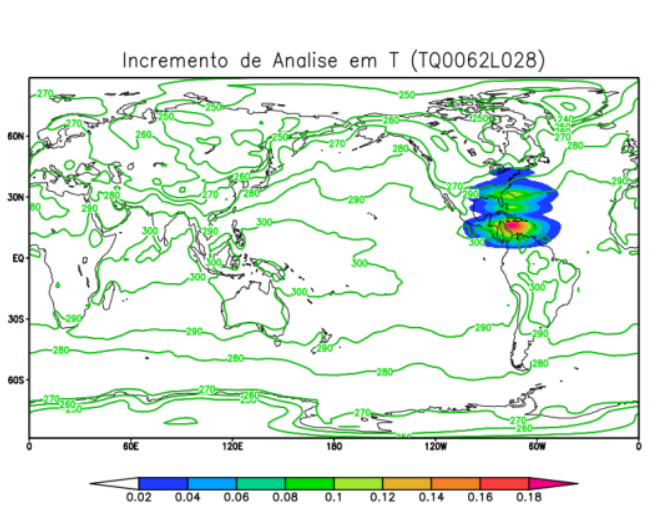
\includegraphics[width=8cm]{./figs/cap3/t_lat_lon-ref.png}
%     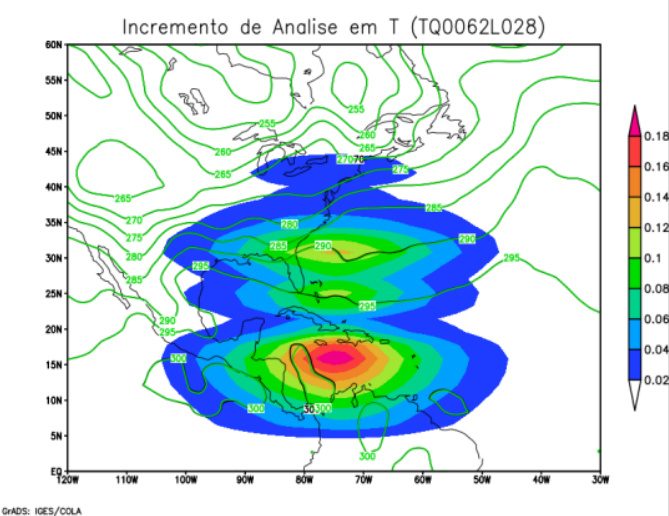
\includegraphics[width=8cm]{./figs/cap3/t_lat_lon-ref_zoom.png}
%     \\
%     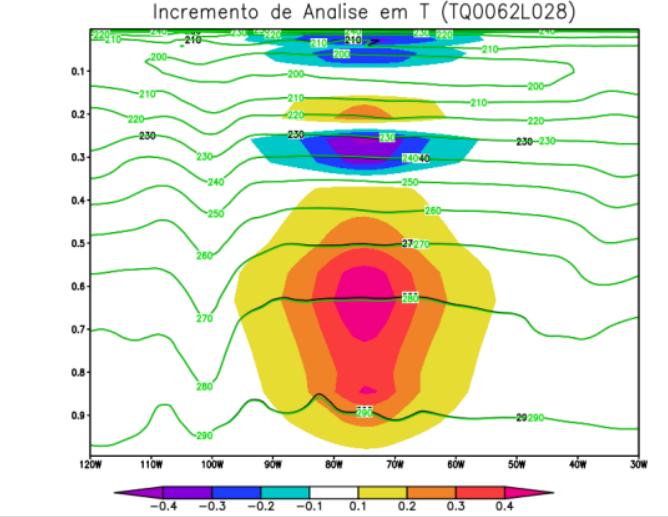
\includegraphics[width=8cm]{./figs/cap3/t_sig_lon-ref.png}
%     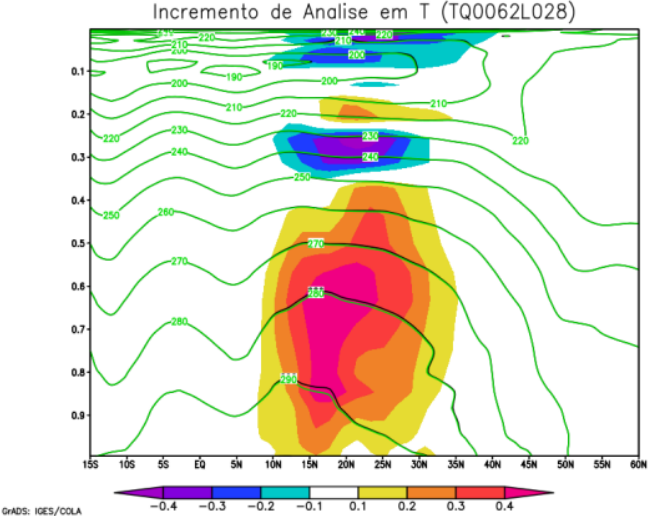
\includegraphics[width=8cm]{./figs/cap3/t_sig_lat-ref.png}
% \end{figure}

% \newpage

\subsection{Correlações entre B CPTEC X NCEP}
\label{sec:simi_B-cptec_ncep}

Aproveitando-se do fato de que a matriz de covariâncias do CPTEC na resolução TQ0299L064 utilizando os pares de previsões de 48 e 24 horas do MCGAv4 foi calculada com dimensões de grade iguais as da matriz de covariâncias do NCEP, então é possível fazer uma comparação direta. A matriz de covariâncias global do NCEP - e que esteve em uso por um breve período na operação do sistema G3DVAR (v1.1.3) no CPTEC, foi calculada com base nos pares de previsões do modelo GFS. Ambos os modelos, MCGAv4 e GFS, são modelos espectrais e as mesmas variáveis foram utilizadas para o cálculo das matrizes de covariâncias. A comparação entre as duas matrizes foi feita a partir do diagrama de espalhamento considerando a distribuição das médias latitudinais nos 64 níveis de cada variável. Nas comparações feitas a seguir, foram consideradas as variáveis $\psi$, $\chi$, $T$ e $q$ nas regiões Hemisfério Norte (HN - lons: 0-360; lats:20N-80N), Trópicos (TR - lons:0-360; lats:20S-20N) e Hemisfério Sul (HS - lons:0-360; lats: 80S-20S). O particionamento em regiões para esta comparação, tem como objetivo melhorar a identificação das correlações entre as variáveis indicadas. Para cada figura, foram calculadas a curva de ajuste, o erro quadrático ($r^{2}$) e o coeficiente de correlação de Pearson ($r$).

Na Figura \ref{fig:disper_Allz_hn_tr_hs}, são apresentados diagramas de dispersão entre as matrizes de covariâncias do NCEP e CPTEC (todos os horários, AllZ), para as variáveis $\psi$, $\chi$, $T$ e $q$, sobre as regiões HN, TR e HS. Em geral, a correlação entre as quantidades consideradas das duas matrizes de covariâncias apresentam valores em torno de 0,9 (90\%), o que reflete as semelhanças encontradas nas amplitudes apresentadas na seção anterior. Além disso, maiores correlações foram encontradas sobre o Hemisfério Sul, enquanto que sobre a região Tropical, foram encontradas as menores correlações. As variáveis que possuem a maior correlação são a função de corrente ($\psi$) e a velocidade potencial ($\chi$) sobre o Hemisfério Sul (Figuras \ref{fig:disper_sfAllz_sh} e \ref{fig:disper_vpAllz_sh}). Entretanto, verificou-se também que as amplitudes de $q$ apresentam os menores valores de correlação e maior erro nos níveis mais altos do modelo. Isto indica que há uma discrepância na representação da umidade a partir do nível 22 (nível sigma 0,604374, aproximadamente 618,88 hPa) até o topo do modelo sobre o Hemisfério Norte. Sobre os Trópicos, as discrepâncias na representação das amplitudes da umidade, estão em níveis mais baixo. Para a umidade, a correlação sobre esta região é de 0,511 (aproximadamente 51\% - Figura \ref{fig:disper_qAllz_tr}). Entretanto, sobre o Hemisfério Sul, a correlação entre as amplitudes da umidade das duas matrizes é alta (aproximadamente 90\%). Sobre esta região, as maiores diferenças estão nos níveis médios. Nas Tabelas \ref{tab:disper_vals_BcptecXncep-sfvp} e \ref{tab:disper_vals_BcptecXncep-Tq}, estão sumarizados os valores de correlação e erro quadrático calculados para todos os horários sinóticos individuais. Neste caso, ressalta-se que as matrizes calculadas para os horários das 00, 06, 12 e 18Z, foram correlacionadas para as regiões indicadas com a matriz de covariâncias do NCEP.

\begin{table}[H]
\caption{Coeficiente de Correlação de Pearson ($r$) e Erro Quadrático ($r^{2}$) para as amplitudes de $\psi$ e $\chi$, entre as matrizes $\mathbf{B}$ CPTEC e NCEP (TQ0299L064) sobre as regiões HN, TR e HS e para os horários AllZ (todos) e 00Z, 06, 12Z e 18Z. Em vermelho, estão destacados os valores de correlação menores do que 0,9.}
\begin{center}
\begin{adjustbox}{max width=\textwidth}
\begin{tabular}{rcccccccccccc}
\toprule
\toprule
        & \multicolumn{6}{c}{$\psi$} & \multicolumn{6}{c}{$\chi$} \\
\cmidrule(lr{.75em}){2-7} \cmidrule(lr{.75em}){8-13}
        & \multicolumn{2}{c}{\textbf{HN}} & \multicolumn{2}{c}{\textbf{TR}} & \multicolumn{2}{c}{\textbf{HS}} & \multicolumn{2}{c}{\textbf{HN}} & \multicolumn{2}{c}{\textbf{TR}} & \multicolumn{2}{c}{\textbf{HS}} \\ 
\cmidrule(lr{.75em}){2-3} \cmidrule(lr{.75em}){4-5} \cmidrule(lr{.75em}){6-7} \cmidrule(lr{.75em}){8-9} \cmidrule(lr{.75em}){10-11} \cmidrule(lr{.75em}){12-13}   
           & $r$ & $r^{2}$ & $r$ & $r^{2}$ & $r$ & $r^{2}$ & $r$ & $r^{2}$ & $r$ & $r^{2}$ & $r$ & $r^{2}$\\ 
\midrule
\textbf{00Z}  & 0,972 & 0,945 & 0,925 & 0,855 & 0,953 & 0,908 & 0,979 & 0,959 & 0,977 & 0,955 & 0,972 & 0,946 \\
\textbf{06Z}  & 0,966 & 0,933 & 0,934 & 0,873 & 0,962 & 0,925 & 0,976 & 0,952 & 0,972 & 0,946 & 0,974 & 0,950 \\
\textbf{12Z}  & 0,975 & 0,951 & 0,940 & 0,885 & 0,963 & 0,927 & 0,978 & 0,956 & 0,977 & 0,955 & 0,970 & 0,941 \\
\textbf{18Z}  & 0,977 & 0,955 & 0,932 & 0,870 & 0,965 & 0,931 & 0,971 & 0,944 & 0,978 & 0,957 & 0,973 & 0,947 \\
\textbf{AllZ} & 0,958 & 0,918 & \textcolor{red}{0,828} & 0,686 & 0,989 & 0,979 & 0,947 & 0,897 & 0,921 & 0,848 & 0,965 & 0,932 \\
\bottomrule     
\end{tabular}
\end{adjustbox}
\end{center}
\label{tab:disper_vals_BcptecXncep-sfvp}
\end{table}

\begin{table}[H]
\caption{Idem Tabela \ref{tab:disper_vals_BcptecXncep-sfvp}, para as variáveis temperatura ($T$) e umidade ($q$).}
\begin{center}
\begin{adjustbox}{max width=\textwidth}
\begin{tabular}{rcccccccccccc}
\toprule
\toprule
        & \multicolumn{6}{c}{$T$} & \multicolumn{6}{c}{$q$} \\
\cmidrule(lr{.75em}){2-7} \cmidrule(lr{.75em}){8-13}
        & \multicolumn{2}{c}{\textbf{HN}} & \multicolumn{2}{c}{\textbf{TR}} & \multicolumn{2}{c}{\textbf{HS}} & \multicolumn{2}{c}{\textbf{HN}} & \multicolumn{2}{c}{\textbf{TR}} & \multicolumn{2}{c}{\textbf{HS}} \\ 
\cmidrule(lr{.75em}){2-3} \cmidrule(lr{.75em}){4-5} \cmidrule(lr{.75em}){6-7} \cmidrule(lr{.75em}){8-9} \cmidrule(lr{.75em}){10-11} \cmidrule(lr{.75em}){12-13}
           & $r$ & $r^{2}$ & $r$ & $r^{2}$ & $r$ & $r^{2}$ & $r$ & $r^{2}$ & $r$ & $r^{2}$ & $r$ & $r^{2}$\\ 
\midrule 
\textbf{00Z}  & 0,966 & 0,934 & 0,985 & 0,970 & 0,966 & 0,934 & \textcolor{red}{0,879} & 0,773 & \textcolor{red}{0,761} & 0,579 & 0,942 & 0,888 \\
\textbf{06Z}  & 0,965 & 0,932 & 0,983 & 0,967 & 0,963 & 0,928 & \textcolor{red}{0,878} & 0,771 & \textcolor{red}{0,761} & 0,579 & 0,945 & 0,893 \\
\textbf{12Z}  & 0,964 & 0,931 & 0,984 & 0,969 & 0,962 & 0,927 & \textcolor{red}{0,883} & 0,781 & \textcolor{red}{0,758} & 0,575 & 0,944 & 0,892 \\
\textbf{18Z}  & 0,966 & 0,935 & 0,985 & 0,971 & 0,965 & 0,932 & \textcolor{red}{0,881} & 0,777 & \textcolor{red}{0,756} & 0,572 & 0,945 & 0,893 \\
\textbf{AllZ} & 0,929 & 0,863 & 0,962 & 0,927 & 0,947 & 0,897 & \textcolor{red}{0,867} & 0,752 & \textcolor{red}{0,715} & 0,511 & 0,953 & 0,909 \\
\bottomrule                                        
\end{tabular}
\end{adjustbox}
\end{center}
\label{tab:disper_vals_BcptecXncep-Tq}
\end{table}

\begin{figure}[H]
    \vspace{-6mm}
    \caption{Diagramas de dispersão entre as amplitudes representadas nas matrizes de covariâncias $\mathbf{B}$ CPTEC e NCEP.}
    \begin{center}
        \subfigure[$\psi$ AllZ (HN)]{
            \label{fig:disper_sfAllz_hn}
            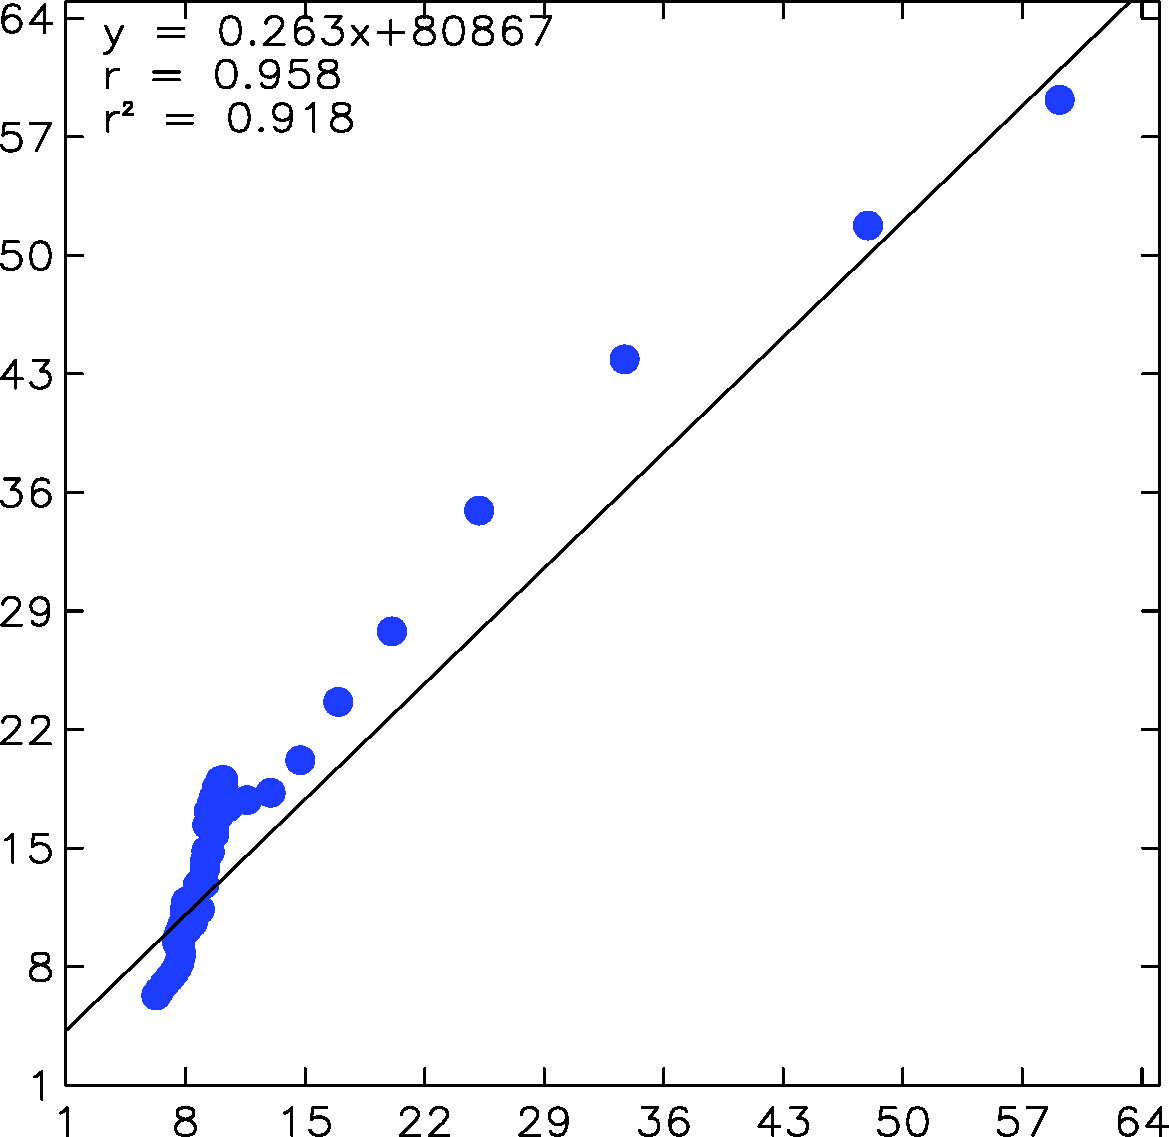
\includegraphics[width=0.3\textwidth,angle=0]{./figs/cap3/disper_novas/scatter-indiv_sf_NH_cptecAllZ_ncep-crop-rotated270.pdf}
        }
        \subfigure[$\psi$ AllZ (TR)]{
           \label{fig:disper_sfAllz_tr}
           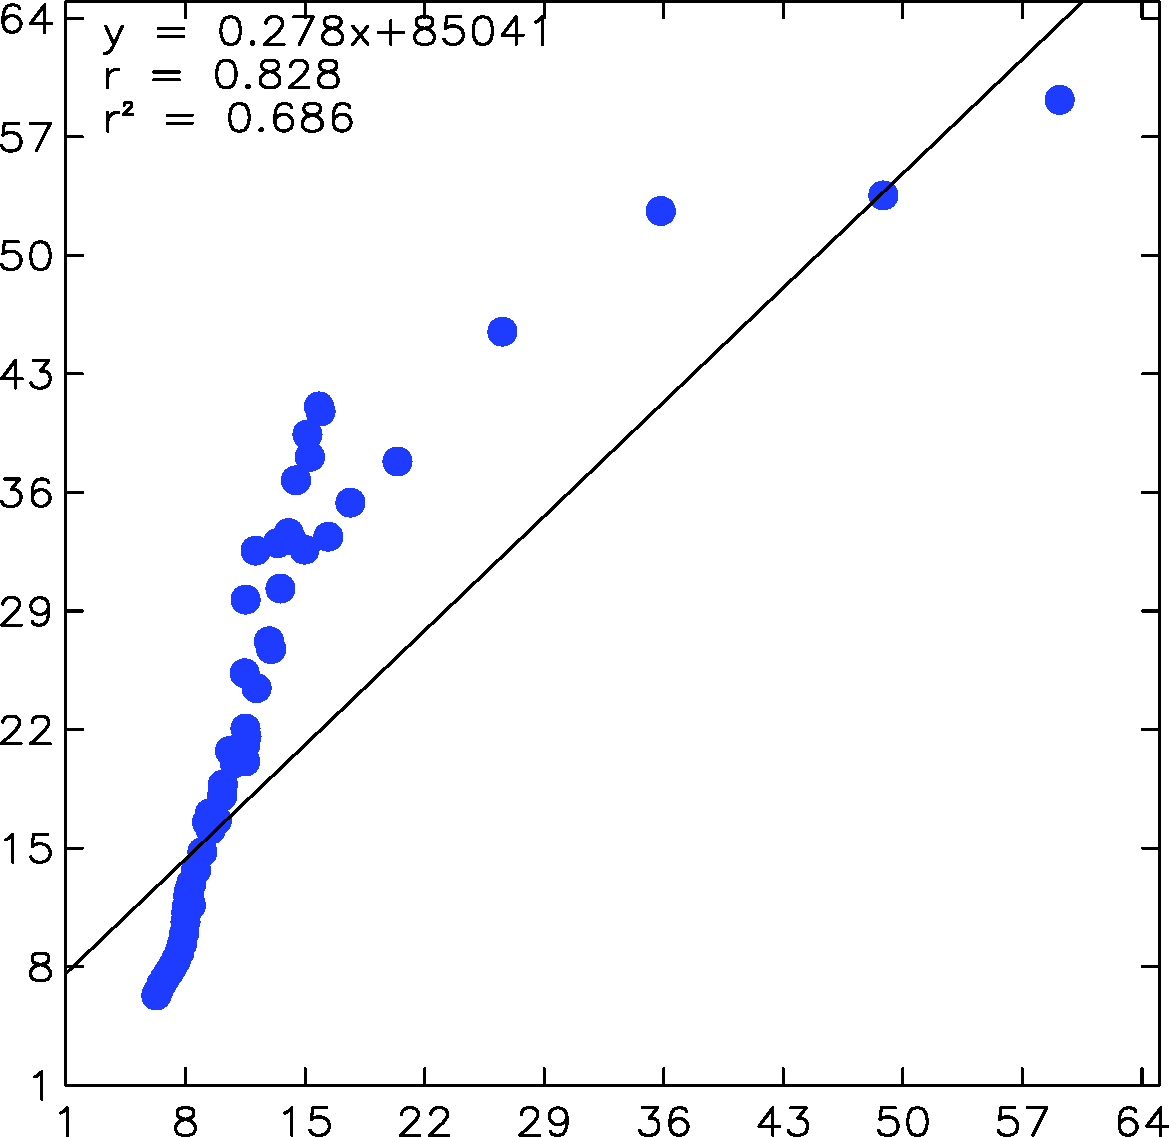
\includegraphics[width=0.3\textwidth,angle=0]{./figs/cap3/disper_novas/scatter-indiv_sf_TR_cptecAllZ_ncep-crop-rotated270.pdf}
        }
        \subfigure[$\psi$ AllZ (HS)]{
           \label{fig:disper_sfAllz_sh}
           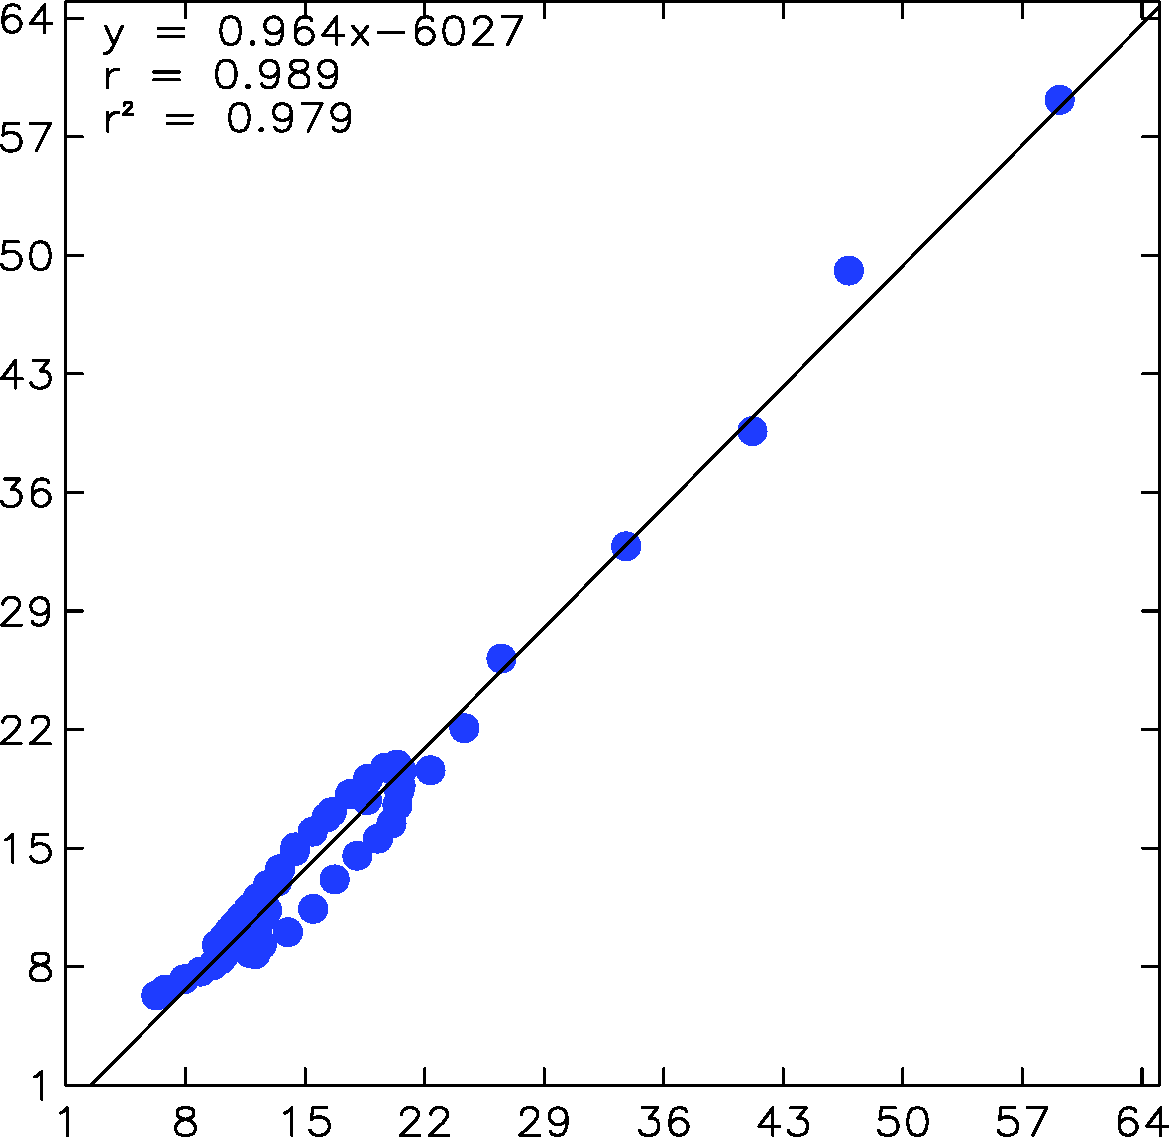
\includegraphics[width=0.3\textwidth,angle=0]{./figs/cap3/disper_novas/scatter-indiv_sf_SH_cptecAllZ_ncep-crop-rotated270.pdf}
        }\\     
        \subfigure[$\chi$ AllZ (HN)]{
            \label{fig:disper_vpAllz_hn}
            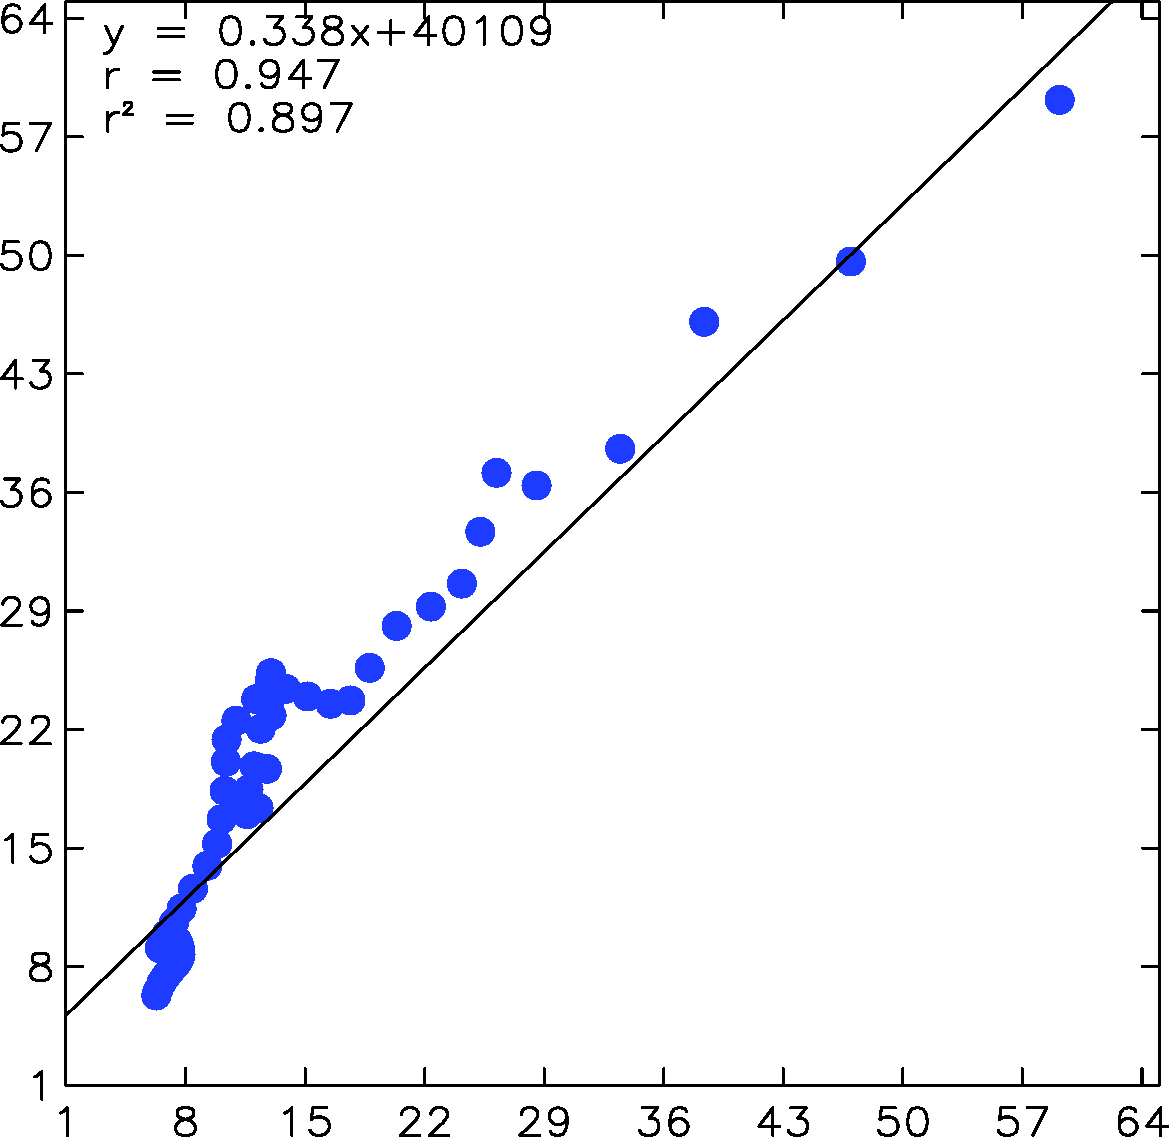
\includegraphics[width=0.3\textwidth,angle=0]{./figs/cap3/disper_novas/scatter-indiv_vp_NH_cptecAllZ_ncep-crop-rotated270.pdf}
        }
        \subfigure[$\chi$ AllZ (TR)]{
           \label{fig:disper_vpAllz_tr}
           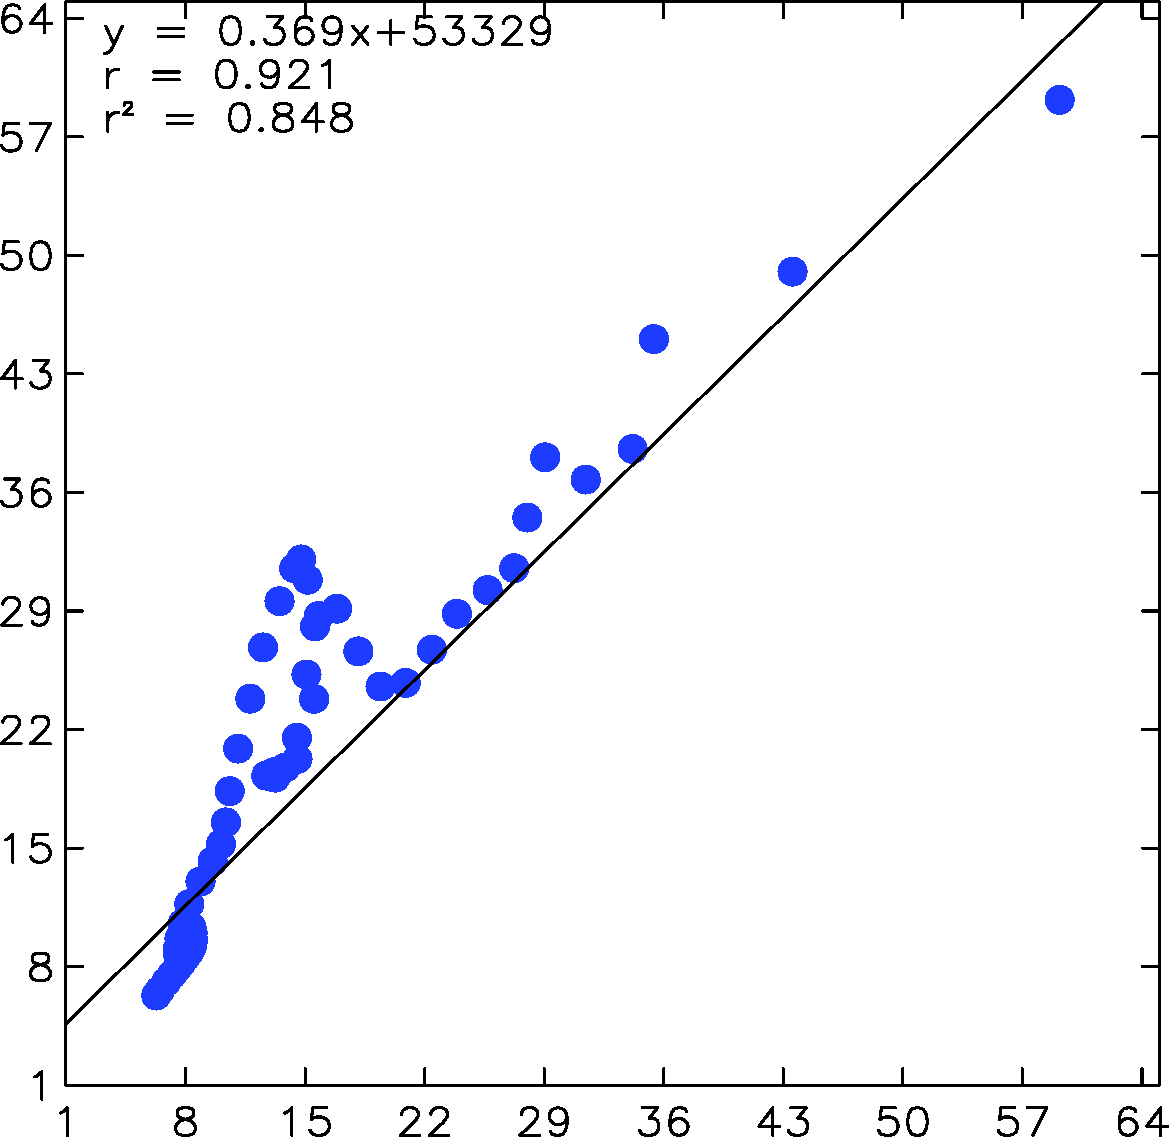
\includegraphics[width=0.3\textwidth,angle=0]{./figs/cap3/disper_novas/scatter-indiv_vp_TR_cptecAllZ_ncep-crop-rotated270.pdf}
        }
        \subfigure[$\chi$ AllZ (HS)]{
            \label{fig:disper_vpAllz_sh}
            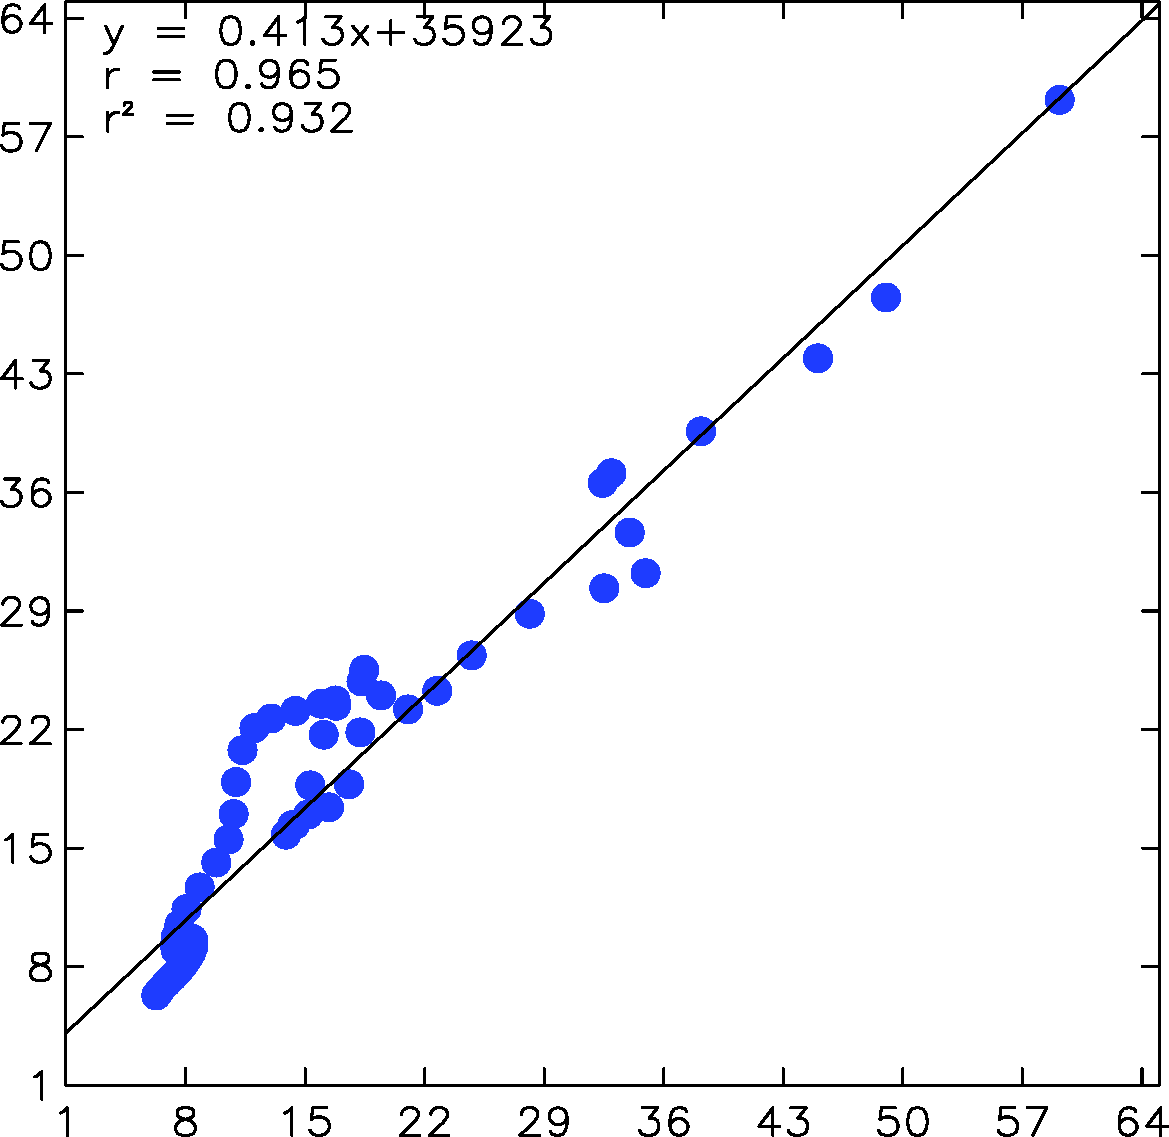
\includegraphics[width=0.3\textwidth,angle=0]{./figs/cap3/disper_novas/scatter-indiv_vp_SH_cptecAllZ_ncep-crop-rotated270.pdf}
        }\\
        \subfigure[$T$ AllZ (HN)]{
            \label{fig:disper_TAllz_hn}
            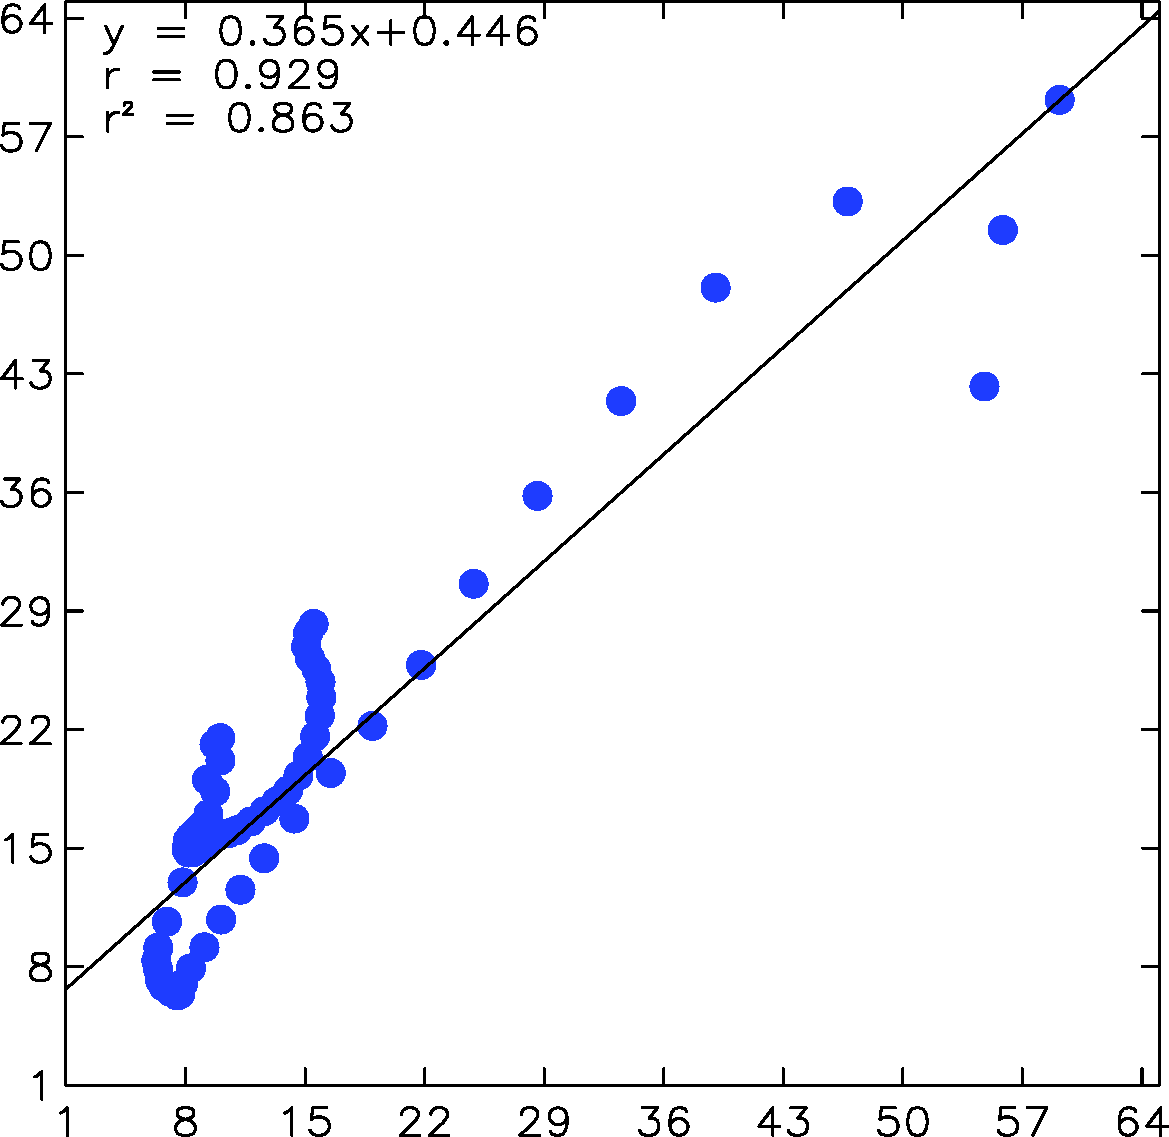
\includegraphics[width=0.3\textwidth,angle=0]{./figs/cap3/disper_novas/scatter-indiv_t_NH_cptecAllZ_ncep-crop-rotated270.pdf}
        }
        \subfigure[$T$ AllZ (TR)]{
           \label{fig:disper_TAllz_tr}
           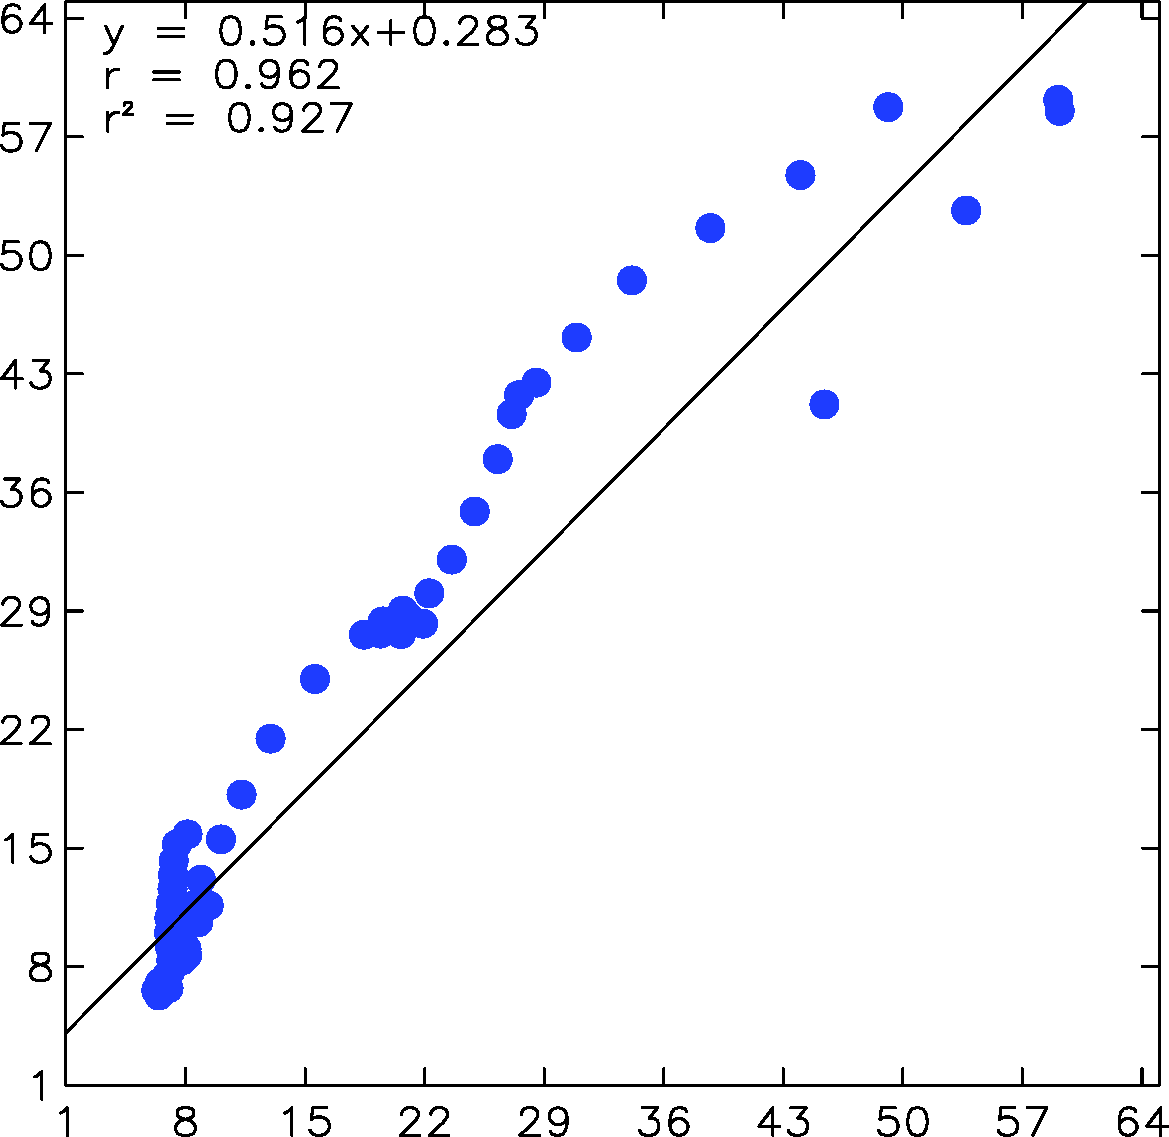
\includegraphics[width=0.3\textwidth,angle=0]{./figs/cap3/disper_novas/scatter-indiv_t_TR_cptecAllZ_ncep-crop-rotated270.pdf}
        }
        \subfigure[$T$ AllZ (HS)]{
            \label{fig:disper_TAllz_sh}
            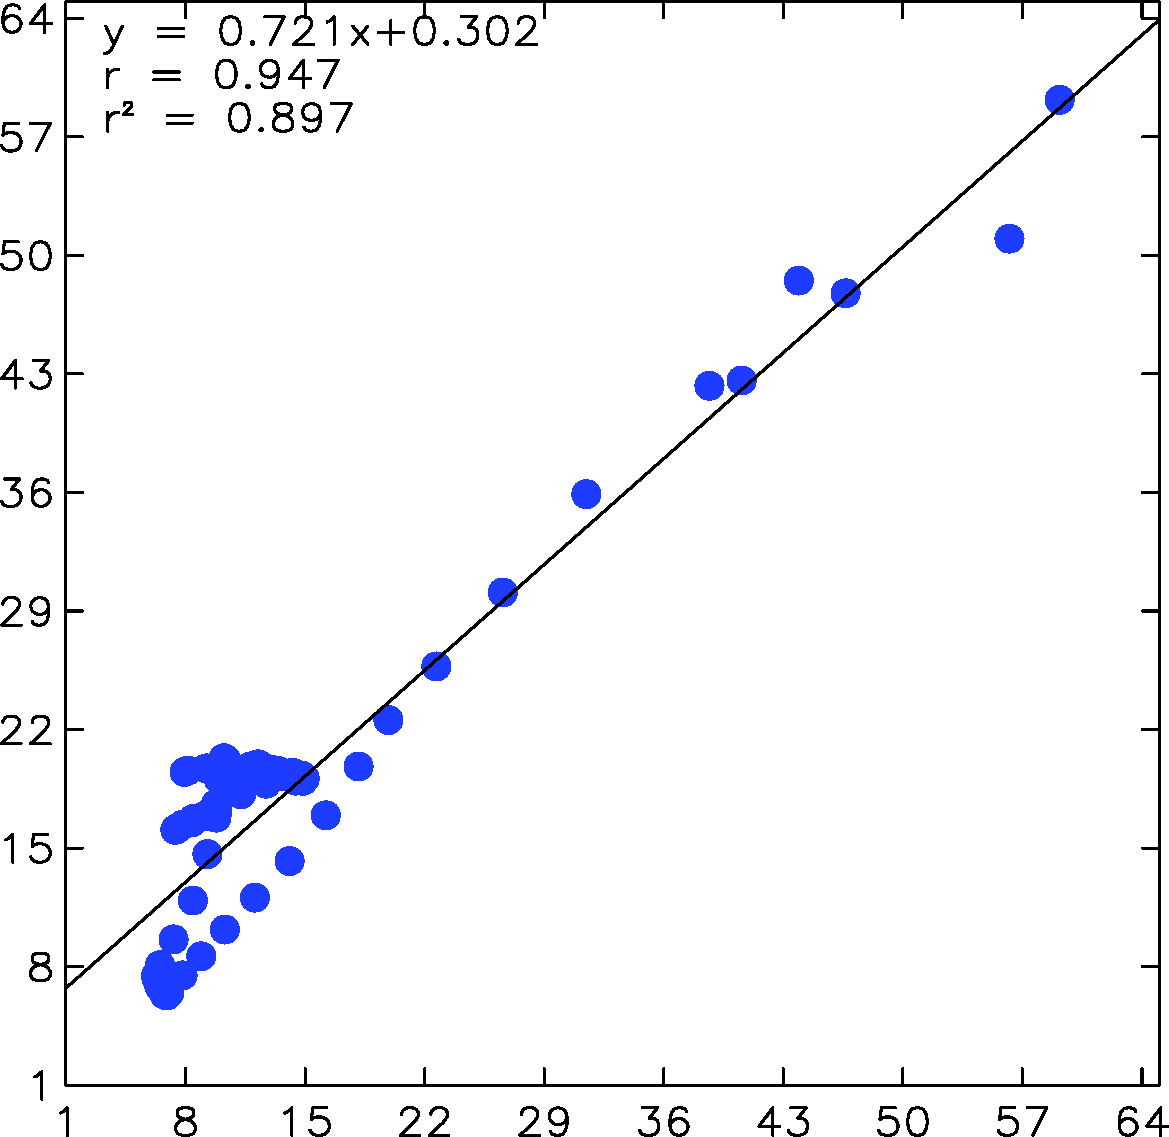
\includegraphics[width=0.3\textwidth,angle=0]{./figs/cap3/disper_novas/scatter-indiv_t_SH_cptecAllZ_ncep-crop-rotated270.pdf}
        }\\
        \subfigure[$q$ AllZ (HN)]{
            \label{fig:disper_qAllz_hn}
            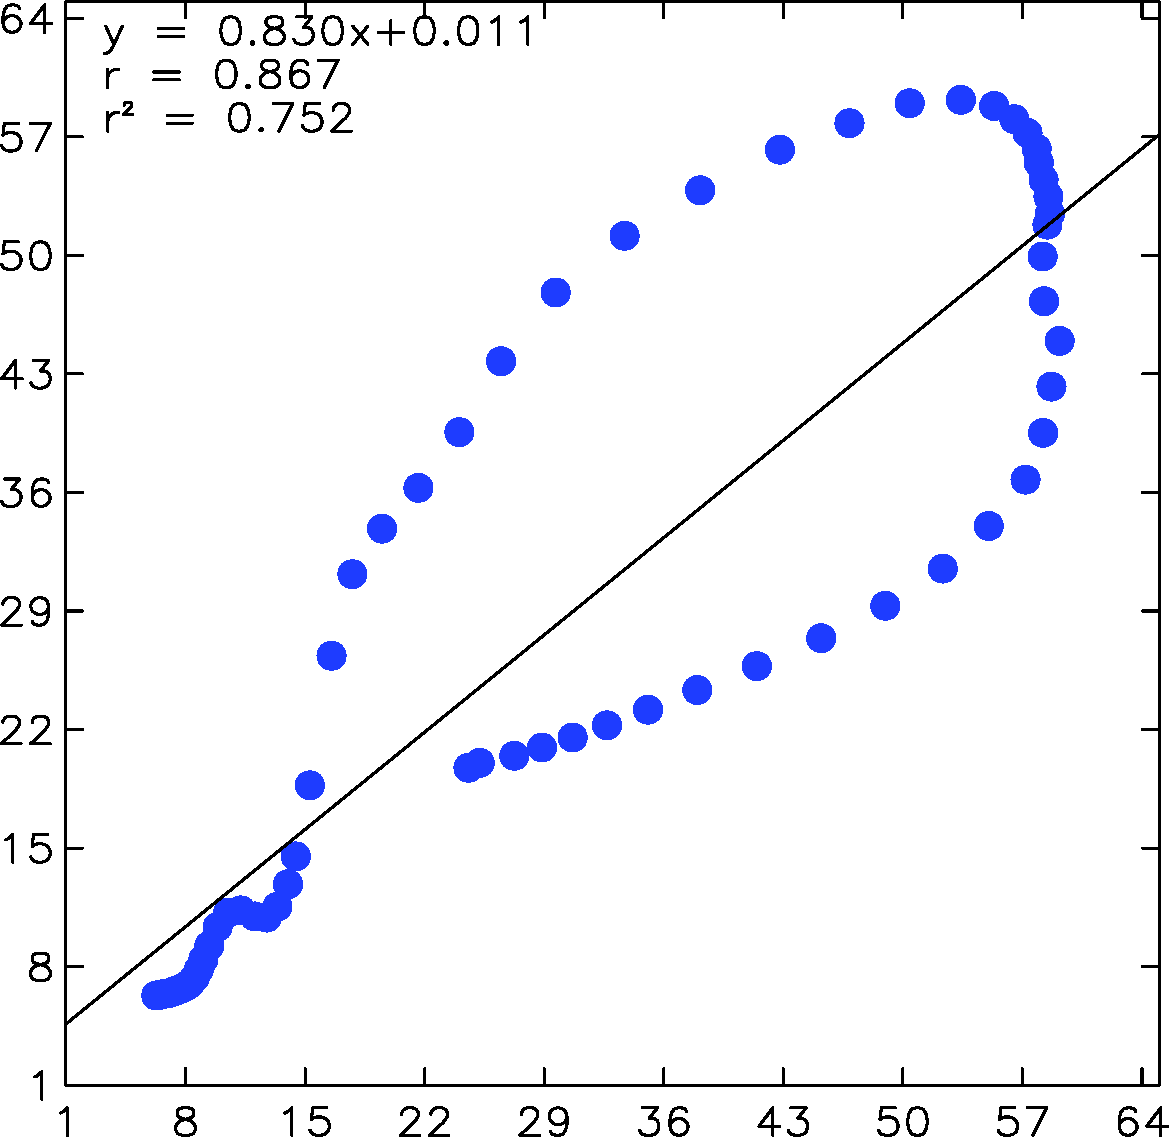
\includegraphics[width=0.3\textwidth,angle=0]{./figs/cap3/disper_novas/scatter-indiv_q_NH_cptecAllZ_ncep-crop-rotated270.pdf}
        }
        \subfigure[$q$ AllZ (TR)]{
           \label{fig:disper_qAllz_tr}
           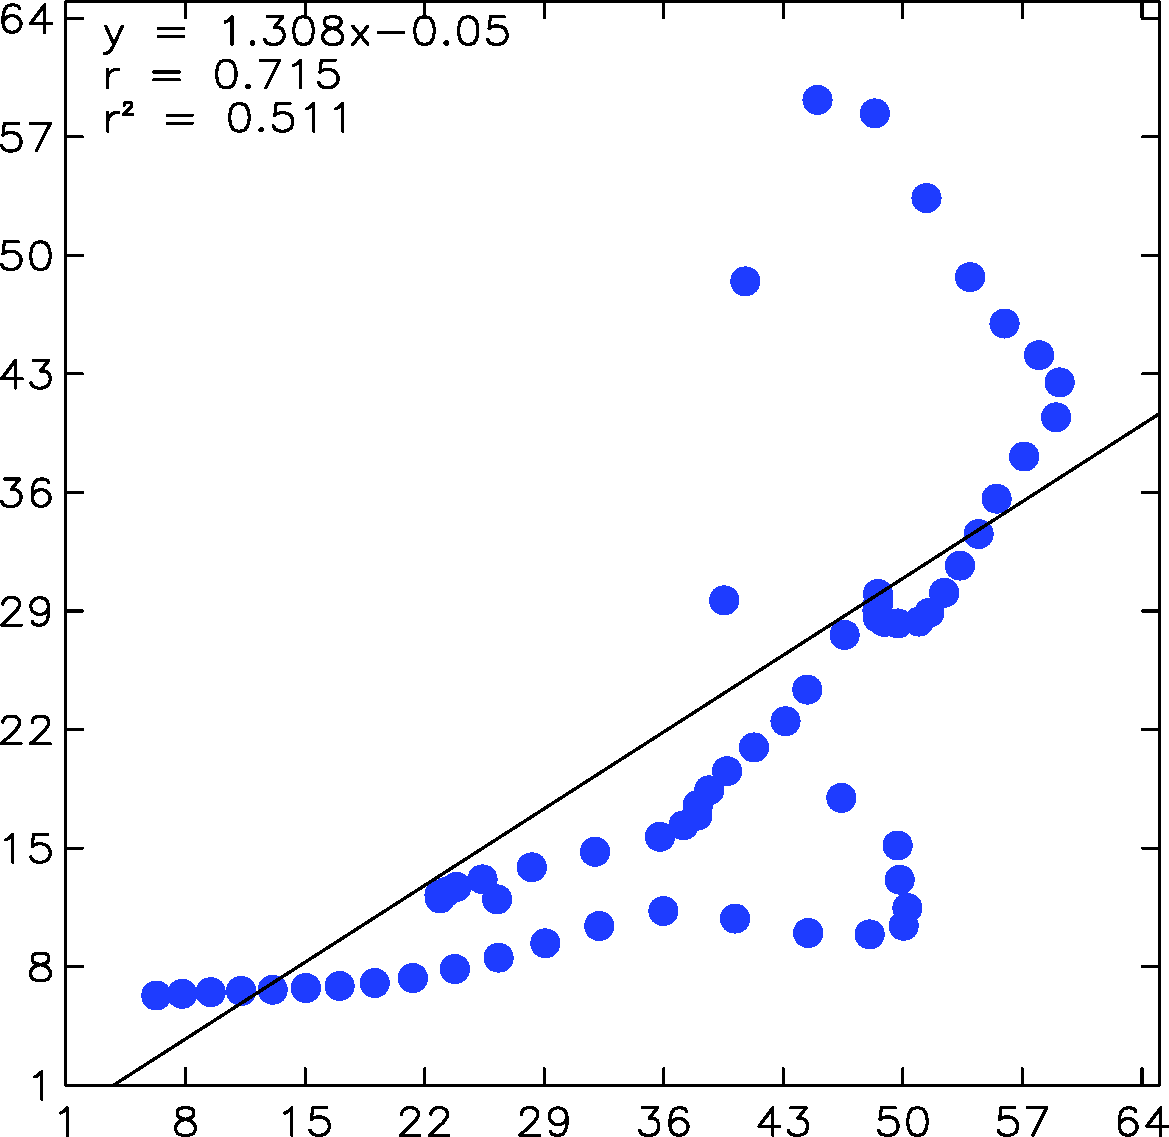
\includegraphics[width=0.3\textwidth,angle=0]{./figs/cap3/disper_novas/scatter-indiv_q_TR_cptecAllZ_ncep-crop-rotated270.pdf}
        }
        \subfigure[$q$ AllZ (HS)]{
           \label{fig:disper_qAllz_sh}
           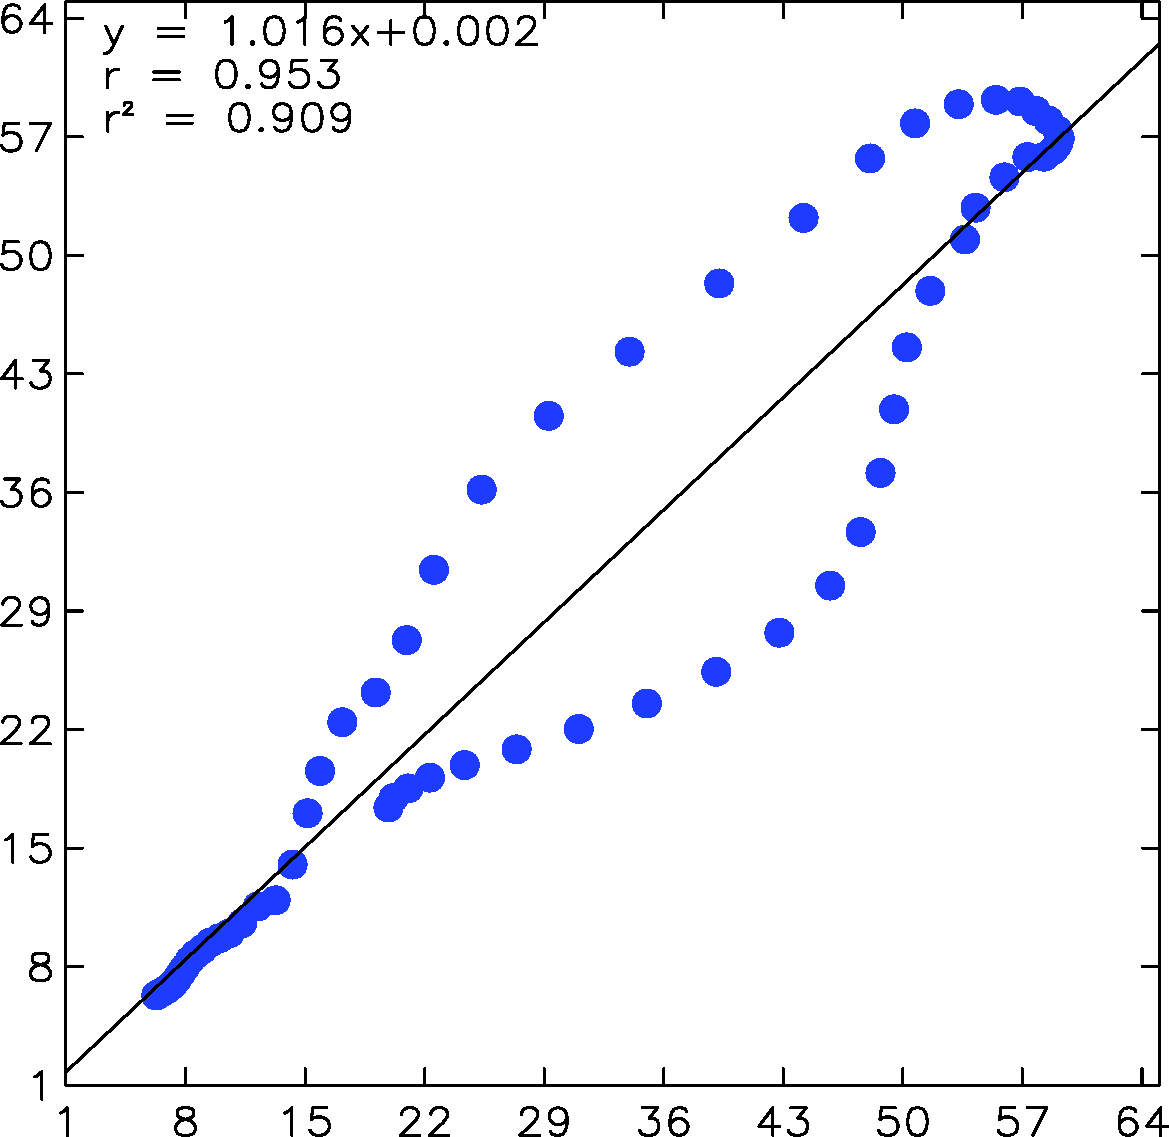
\includegraphics[width=0.3\textwidth,angle=0]{./figs/cap3/disper_novas/scatter-indiv_q_SH_cptecAllZ_ncep-crop-rotated270.pdf}
        }
  \end{center}
  \vspace{2mm}
  \legenda{Diagramas de dispersão (níveis sigma), correlações e erros quadráticos entre as amplitudes representadas nas matrizes de covariâncias $\mathbf{B}$ CPTEC e NCEP em todos os horários (AllZ), para as regiões HN (coluna a esquerda), TR (coluna do meio) e HS (coluna da direita).}
  \label{fig:disper_Allz_hn_tr_hs}
  \vspace{-4mm}
  \FONTE{Produção do autor.}
\end{figure}

\section{Aspecto do Incremento de Análise}

Como forma de verificação da influência e do impacto que a nova matriz de covariâncias do CPTEC exerce no incremento de análise do sistema G3DVAR, foi feito um experimento com a assimilação de uma única observação (sintética) no sistema. As Figuras \ref{fig:t_incr_Bcptec} e \ref{fig:t_incr_Bncep} apresentam uma comparação entre os incrementos de análise produzidos pelas matrizes de covariâncias do CPTEC e do NCEP (respectivamente).

Na Figura \ref{fig:t_incr_Bcptec}, é mostrado o incremento de análise (Previsão subtraída da Análise, ou OmA) produzido pela assimilação de uma observação sintética de vento zonal em 1000hPa. Para isto, ajustou-se o erro da observação para 1 $ms^{-1}$, bem como a magnitude da inovação trazida pela observação (Previsão subtraída da Observação, ou OmF). Neste caso, o painel da esquerda mostra o incremento de análise isotrópico (em que os pesos dados para o Filtro Recursivo nas direções $x$ e $y$ são iguais), de forma que o incremento produzido possui aspecto quase igual em todas as direções. O formato achatado no topo evidencia apenas o fato de que a observação foi posicionada mais próxima ao polo norte, mais precisamente no ponto com coordenada 0 (longitude) e 45N (latitude). No painel da direita, o incremento de análise mostrado é anisotrópico, e os parâmetros principais ajustados no GSI para a sua produção, são apresentados na Tabela \ref{tab:ajusteB}:

\begin{table}[H]
\caption{Parâmetros de configuração utilizados no sistema GSI para a aplicação das matrizes de covariâncias do CPTEC e do NCEP.}
\begin{center}
\begin{adjustbox}{max width=\textwidth}
\begin{tabular}{>{\centering\bfseries}m{2.5cm} >{\centering}m{2.5cm} >{\centering\arraybackslash}m{10cm}}
\toprule
\toprule
\multicolumn{1}{c}{\textbf{Parâmetro}} & \multicolumn{1}{c}{\textbf{Valor}} & \multicolumn{1}{c}{\textbf{Descrição}} \\
\midrule
$vs$            & 0,7             & Fator de escala do comprimento de correlação vertical \\ 
$hzscl$         & 1,7; 0,8; 0,5   & Fator de suavização para as 3 escalas horizontais \\ 
$hswgt$         & 0,45; 0,3; 0,25 & Pesos aplicados a cada escala horizontal \\ 
$bw$            & 0               & Fator no cálculo da covariância do erro \\ 
$norsp$         & 4               & Ordem de suavização horizontal das covariâncias do erro de previsão \\ 
$bkg\_flowdep$  & True/False      & Flag para usar (True = anisotrópico) ou não (False = isotrópico) a dependência das variâncias do erro de previsão \\
\bottomrule
\end{tabular}
\end{adjustbox}
\end{center}
\label{tab:ajusteB}
\end{table}

O parâmetro ``$vs$'', ajusta a escala vertical e sua unidade é dada em pontos de grade; o parâmetro ``$hzscl$'', ajusta a escala horizontal e o parâmetro ``$hswgt$'' ajusta os pesos dados a aplicação do filtro recursivo nas direções $x$, $y$ e $z$, respectivamente.

\begin{figure}[H]
    \vspace{2mm}
    \caption{Aspectos dos incrementos de análise utilizando a nova matriz de covariâncias do CPTEC.}
    \begin{center}
        \subfigure[$\mathbf{B}$ CPTEC lat x lon (Isotrópica)]{
            \label{fig:t_incr_Bcptec_lat_lon_iso}
            \includegraphics[width=0.47\textwidth]{./figs/cap3/incrementos_novas/incr_bcptec_iso_lat_lon-crop-rotated270.pdf}
        }     
        \subfigure[$\mathbf{B}$ CPTEC lat x lon (Anisotrópica)]{
            \label{fig:t_incr_Bcptec_lat_lon_aniso}
            \includegraphics[width=0.47\textwidth]{./figs/cap3/incrementos_novas/incr_bcptec_aniso_lat_lon-crop-rotated270.pdf}
        }\\
        \subfigure[$\mathbf{B}$ CPTEC lat x lev (Isotrópica)]{
            \label{fig:t_incr_Bcptec_lat_lev_iso}
            \includegraphics[width=0.47\textwidth]{./figs/cap3/incrementos_novas/incr_bcptec_iso_lat_lev-crop-rotated270.pdf}
        }
        \subfigure[$\mathbf{B}$ CPTEC lat x lev (Anisotrópica)]{
           \label{fig:t_incr_Bcptec_lat_lev_aniso}
           \includegraphics[width=0.47\textwidth]{./figs/cap3/incrementos_novas/incr_bcptec_aniso_lat_lev-crop-rotated270.pdf}
        }\\
        \subfigure[$\mathbf{B}$ CPTEC lon x lev (Isotrópica)]{
            \label{fig:t_incr_Bcptec_lon_lev_iso}
            \includegraphics[width=0.47\textwidth]{./figs/cap3/incrementos_novas/incr_bcptec_iso_lon_lev-crop-rotated270.pdf}
        }
        \subfigure[$\mathbf{B}$ CPTEC lon x lev (Anisotrópica)]{
           \label{fig:t_incr_Bcptec_lon_lev_aniso}
           \includegraphics[width=0.47\textwidth]{./figs/cap3/incrementos_novas/incr_bcptec_aniso_lon_lev-crop-rotated270.pdf}
        }\\
        \includegraphics[width=0.75\textwidth]{./figs/cap3/incrementos_novas/cbar-crop-rotated270.pdf}
    \end{center}
    \vspace{2mm}
    \legenda{Incremento de análise da temperatura ($T$) ano nível de 1000 hPa, utilizando a nova matriz de covariâncias do CPTEC: a esquerda, incremento isotrópico; a direita incremento anisotrópico.}
   \label{fig:t_incr_Bcptec}
   \FONTE{Produção do autor.}
\end{figure}
    
A Figura \ref{fig:t_incr_Bncep} apresenta o incremento de análise produzido pela matriz de covariâncias do NCEP, aplicada ao sistema G3DVAR, assimilando a mesma observação sintética única, no mesmo nível e com as mesmas magnitudes de erro e inovação. De forma geral, para ambos os casos (isotrópico e anisotrópico), o incremento de análise calculado pela matriz de covariâncias do CPTEC (matriz CPTEC BAllZ), produz um incremento mais largo, abrangendo mais pontos de grade em todas as direções. Isso significa que o incremento de análise calculado, é espalhado sobre uma região maior ao redor da vizinhança da observação e que a sua influência pode ser transportada para mais longe. Em uma situação física em que, por exemplo há a incursão de um sistema frontal e, considerando-se o caso anisotrópico, a assimilação de dados pode trazer um benefício importante para a previsão gerada, porque a análise utilizada possuirá um balanço melhor entre observações e previsão. Isso mostra a importância da seleção das observações, do controle de qualidade e do \textit{thinning} do sistema (i.e., o controle espacial das observações). Além disso, a magnitude do incremento de análise produzido pela matriz de covariâncias do CPTEC é mais suave, embora seja menos concentrado. Em contraste, a matriz de covariâncias do NCEP, apresenta incrementos muito mais concentrados e um pouco mais intensos também.    
    
\begin{figure}[H]
    \vspace{2mm}
    \caption{Idem Figura \ref{fig:t_incr_Bcptec}, para a matriz de covariâncias do NCEP.}
    \begin{center}
        \subfigure[$\mathbf{B}$ NCEP lat x lon (Isotrópica)]{
            \label{fig:t_incr_Bncep_lat_lon_iso}
            \includegraphics[width=0.47\textwidth]{./figs/cap3/incrementos_novas/incr_bncep_iso_lat_lon-crop-rotated270.pdf}
        }     
        \subfigure[$\mathbf{B}$ NCEP lat x lon (Anisotrópica)]{
            \label{fig:t_incr_Bncep_lat_lon_aniso}
            \includegraphics[width=0.47\textwidth]{./figs/cap3/incrementos_novas/incr_bncep_aniso_lat_lon-crop-rotated270.pdf}
        }\\
        \subfigure[$\mathbf{B}$ NCEP lat x lev (Isotrópica)]{
            \label{fig:t_incr_Bncep_lat_lev_iso}
            \includegraphics[width=0.47\textwidth]{./figs/cap3/incrementos_novas/incr_bncep_iso_lat_lev-crop-rotated270.pdf}
        }
        \subfigure[$\mathbf{B}$ NCEP lat x lev (Anisotrópica)]{
           \label{fig:t_incr_Bncep_lat_lev_aniso}
           \includegraphics[width=0.47\textwidth]{./figs/cap3/incrementos_novas/incr_bncep_aniso_lat_lev-crop-rotated270.pdf}
        }\\
        \subfigure[$\mathbf{B}$ NCEP lon x lev (Isotrópica)]{
            \label{fig:t_incr_Bncep_lon_lev_iso}
            \includegraphics[width=0.47\textwidth]{./figs/cap3/incrementos_novas/incr_bncep_iso_lon_lev-crop-rotated270.pdf}
        }
        \subfigure[$\mathbf{B}$ NCEP lon x lev (Anisotrópica)]{
           \label{fig:t_incr_Bncep_lon_lev_aniso}
           \includegraphics[width=0.47\textwidth]{./figs/cap3/incrementos_novas/incr_bncep_aniso_lon_lev-crop-rotated270.pdf}
        }\\
        \includegraphics[width=0.75\textwidth]{./figs/cap3/incrementos_novas/cbar-crop-rotated270.pdf}
    \end{center}
    \vspace{2mm}
    \legenda{Incremento de análise da temperatura ($T$) ano nível de 1000 hPa, utilizando a matriz de covariâncias do NCEP: a esquerda, incremento isotrópico; a direita incremento anisotrópico.}
   \label{fig:t_incr_Bncep}
   \FONTE{Produção do autor.}
\end{figure}